%%%%%%%%%%%%%%%%%%%%%%%%%%%%%%%%%%%%%%%%
% datoteka diploma.tex
%
% vzorčna datoteka za pisanje diplomskega dela v formatu LaTeX
% na UL Fakulteti za matematiko in fiziko
%
% vkup spravil Gašper Fijavž, december 2010 množica popravkov v januarju,
% februarju marcu 2011 verzijo 29. marec 2011 za FMF 19.9.2013 prilagodil Rok
% Mihevc
%%%%%%%%%%%%%%%%%%%%%%%%%%%%%%%%%%%%%%%%

\documentclass[a4paper, twoside, 12pt]{book}

\usepackage[utf8]{inputenc}
\usepackage[slovene,english]{babel}    % naloži, med drugim,
\usepackage[pdftex]{graphicx}  % omogoča vlaganje slik
\usepackage{fancyhdr}          % poskrbi, na primer, za
\usepackage{amssymb}           % dodatni simboli
\usepackage{amsmath}           % eqref, npr.
\usepackage{verbatim}
% \usepackage{float}


%oznake strani
\renewcommand{\chaptermark}[1]

\newcommand{\BibTeX}{{\sc Bib}\TeX}
\newcommand{\autfont}{\Large}
\newcommand{\titfont}{\LARGE\bf}
\newcommand{\clearemptydoublepage}{\newpage{\pagestyle{empty}\cleardoublepage}}
%\newcommand{\clearemptydoublepage}{\newpage \thispagestyle{empty}}
\setcounter{tocdepth}{2}

\begin{document}
\selectlanguage{slovene}
\frontmatter
\renewcommand{\thepage}{}

\begin{center}
  {\large\sc Univerza v Ljubljani\\
    Fakulteta za Matematiko in Fiziko\\
    Oddelek za Fiziko\\
  Univerzitetni študij, naravoslovna smer}
  \vskip 10em
  {\autfont Rok Mihevc \par}
  {\titfont Kraške vrtače Dinarskega krasa \par}
  {\vskip 2em \textsc{DIPLOMSKO DELO}\par}
  \vfill
  \null
  {\large \textsc{Mentor}: prof.\ dr.  Rudolf Podgornik\par}
    %  {\large \textsc{Somentor}:  izr.\ prof.\ dr. \par}%
  {\vskip 2em \large Ljubljana, 2014 \par}
\end{center}
\addtocontents{toc}{\vspace{1em}}{}

\mainmatter
\setcounter{page}{3}
\clearemptydoublepage

%\def\thepage{}% preprecimo tezave s stevilkami strani v kazalu

\addcontentsline{toc}{chapter}{Povzetek}
\chapter*{Povzetek}

  Z numeričnimi metodami obdelamo $60 km^2$ velik digitalni model reliefa Menišije ločljivosti $1m^2$ in identificiramo veliko število kraških vrtač. Iz oblik velikega števila vrtač izračunamo povprečno obliko vrtače in jo analitično opišemo z Gaussovo funkcijo. Odkrite realne vrtače nato prilegamo na Gaussovo funkcijo ter pogledamo porazdelitev parametrov le-te na našem vzorcu.

  Zaradi geološke zgodovine področja Menišije in medsebojne podobnosti vrtač na tem območju postavimo tezo, da jih je oblikoval isti geomorfološki proces, ki vodi do vsem skupne stabilne oblike, ki so jo vrtače na tem območju že dosegle.
  S pomočjo podatkov, pridobljenih v prvem delu naloge, predlagamo statičen nastavek, ki analitično opiše najdene vrtače. Postavimo tezo, da vrtače oblikuje stohastična denudacija površja, ter primerjamo teoretično pričakovan eksponent hrapavosti z izmerjenim. Pogledamo še nekaj determinističnih difuzijsko-reakcijskih sistemov, ki bi lahko služili kot dinamični model nastanka vrtač.

\vspace{1cm}

\noindent \textbf{Ključne besede:} Digitalni model reliefa, obdelava slik, vrtača, kras, razvoj reliefa, stohastične diferencialne enačbe, dinamične enačbe
\smallskip

\noindent \textbf{PACS:} 95.75.Mn, 02.50.Ey 02.60.Cb, 02.60.Ed, 68.35.Ct, 68.35.Fx
% \newpage \thispagestyle{empty}
\clearemptydoublepage
\selectlanguage{english}

\addcontentsline{toc}{chapter}{Abstract}
\chapter*{Abstract}

  Using numerical methods we analyzed $60 km^2$ of $1m^2$ resolution digital terrain model of Menišija and identified a large number of karst Dolines. We calculated average shape of a large number of Dolines and analytically described it by a Gaussian function. We then fitted the real Dolines to a Gaussian function and studied the distribution of parameters in our sample from Menišija.

  Due to the geological history of Menišija and similarity of Dolines in the area we propose that they were shaped by the same geomorphological process, that ultimately leads to a common stable form that was already reached by the Dolines in this area.
  Using the data acquired in the second chapter we propose a static Ansatz that describes found Dolines. We propose a thesis that Dolines are formed by stochastic surface denudation, and compare the theoretically derived roughness exponent with the one measured on relief data from Menišija. Then we study several diffusion-reaction systems, which could serve as dynamic models of Dolines.

\vspace{1cm}

\noindent \textbf{Keywords:} Digital relief model, image processing, dolines, karst relief evolution, stochastic differential equations, dynamic equations
\smallskip

\noindent \textbf{PACS:} 95.75.Mn, 02.50.Ey 02.60.Cb, 02.60.Ed, 68.35.Ct, 68.35.Fx
\selectlanguage{slovene}
%\newpage \thispagestyle{empty}
\clearemptydoublepage

\pagestyle{fancy}
\rhead{\thepage}

\tableofcontents{}
\clearemptydoublepage

\chapter{Uvod}
\label{ch:uvod}

Namen tega dela je na podlagi digitalnega modela reliefa dokumentirati in statistično preučiti velik vzorec kraških vrtač na slovenskem Dinarskem krasu, predlagati analitično funkcijo, ki bi opisala idealno vrtačo, ter na podlagi le-te poskusiti modelirati dejavnike, ki povzročajo nastanek in obliko vrtač.

Vrtače so zaobljene lijakaste globeli, globine nekaj metrov in premera nekaj deset metrov. Prvi jih leta 1893 opiše in poimenuje Cvijić \cite{cvijic1893}. Najdemo jih na starih kraških poljih in planotah po celotnem Dinarskem krasu. Medtem ko v literaturi ocene časa potrebnega za nastanek vrtač ne najdemo, v nadaljevanju ta čas ocenimo na 0,5 do 3,5 milijona let. Primer starega polja z razvitimi vrtačami: (Slika \ref{fig:vrtace-bpetrovac}). 

  \begin{figure}[h]
    \begin{center}
      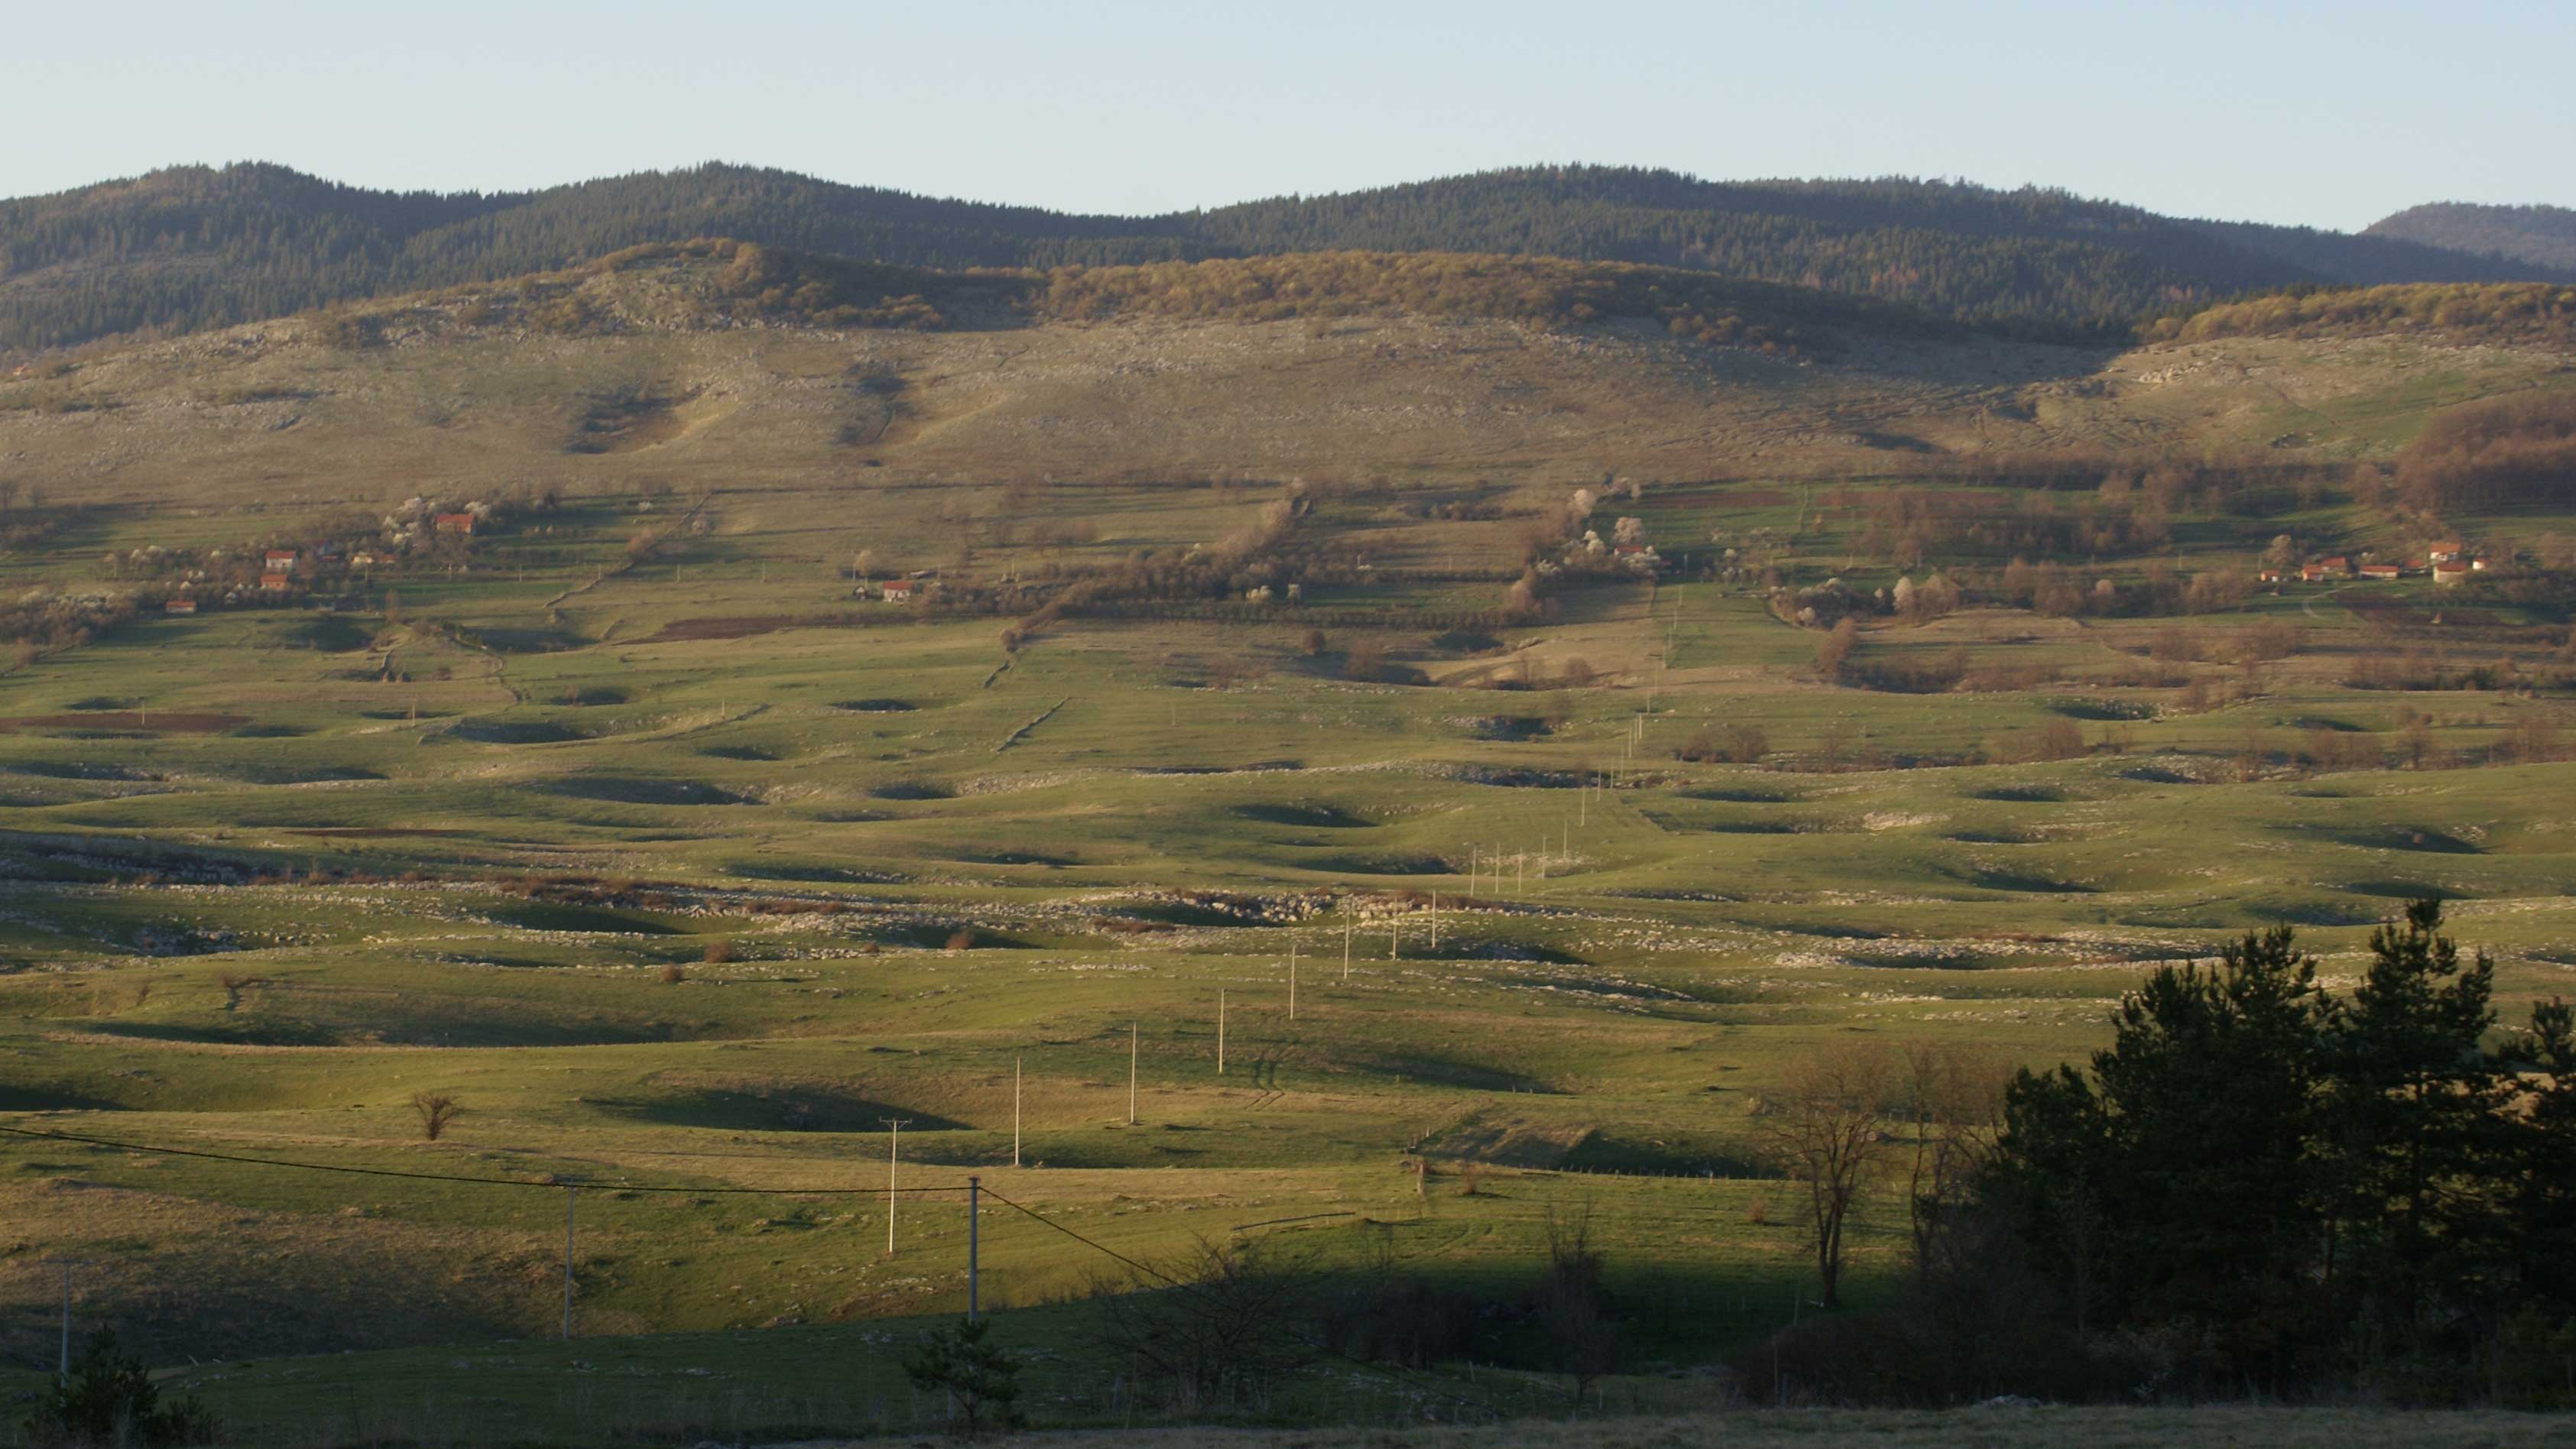
\includegraphics[width=8cm]{slike/bpetrovac}
    \end{center}
    \caption{Skupina vrtač vrezanih v staro kraško polje v bližini Bosanskega Petrovca, BiH \cite{bpetrovac}.}
    \label{fig:vrtace-bpetrovac}
  \end{figure}

Najširše sprejet model nastanka vrtač v geomorfološki literaturi podata Ford in Williams \cite{ford2007karst}. Grobo prevedemo in povzamemo tekst (\cite{ford2007karst}, str. 242) ter skico (Slika \ref{fig:vrtaca-ford-williams}), ki konceptualno opišeta dinamiko vrtač in nam bosta služila kot izhodišče pri študiju:

\begin{quotation}
Skledasta oblika vrtač kaže, da je bilo iz njihovega centra odnešene več kamnine kot z njihovega roba. To nakazuje da je na delu skupen naravni proces, ki fokusira raztapljanje. ... \\
Ko se površje malenkost poglobi, se vzpostavi pozitivna povratna zanka, ki poganja nadaljnje poglabljanje zaradi centripetalnega vodnega toka in posledično korozije. Agresivnost vode se še poveča z biogeno produkcijo $CO_2$ v prsti, ki se ponavadi nabira na dnu depresije. ... \\
Z učinkovitim navpičnim odvajanjem, ki ga omogoči korozijsko razširjanje razpok, se povečuje povprečna hitrost vodnega toka in z njo količina mehansko izprane prsti in kamnine. ... \\
Čeprav je glavna težnja pri nastajanju vrtač samo ojačitev, imajo nekateri efekti negativen povratni vpliv. Na primer, nekatere prsti, ki pokrivajo kras imajo manjšo prepustnost kot živa skala."
\end{quotation}
\begin{figure}[h!]
  \begin{center}
    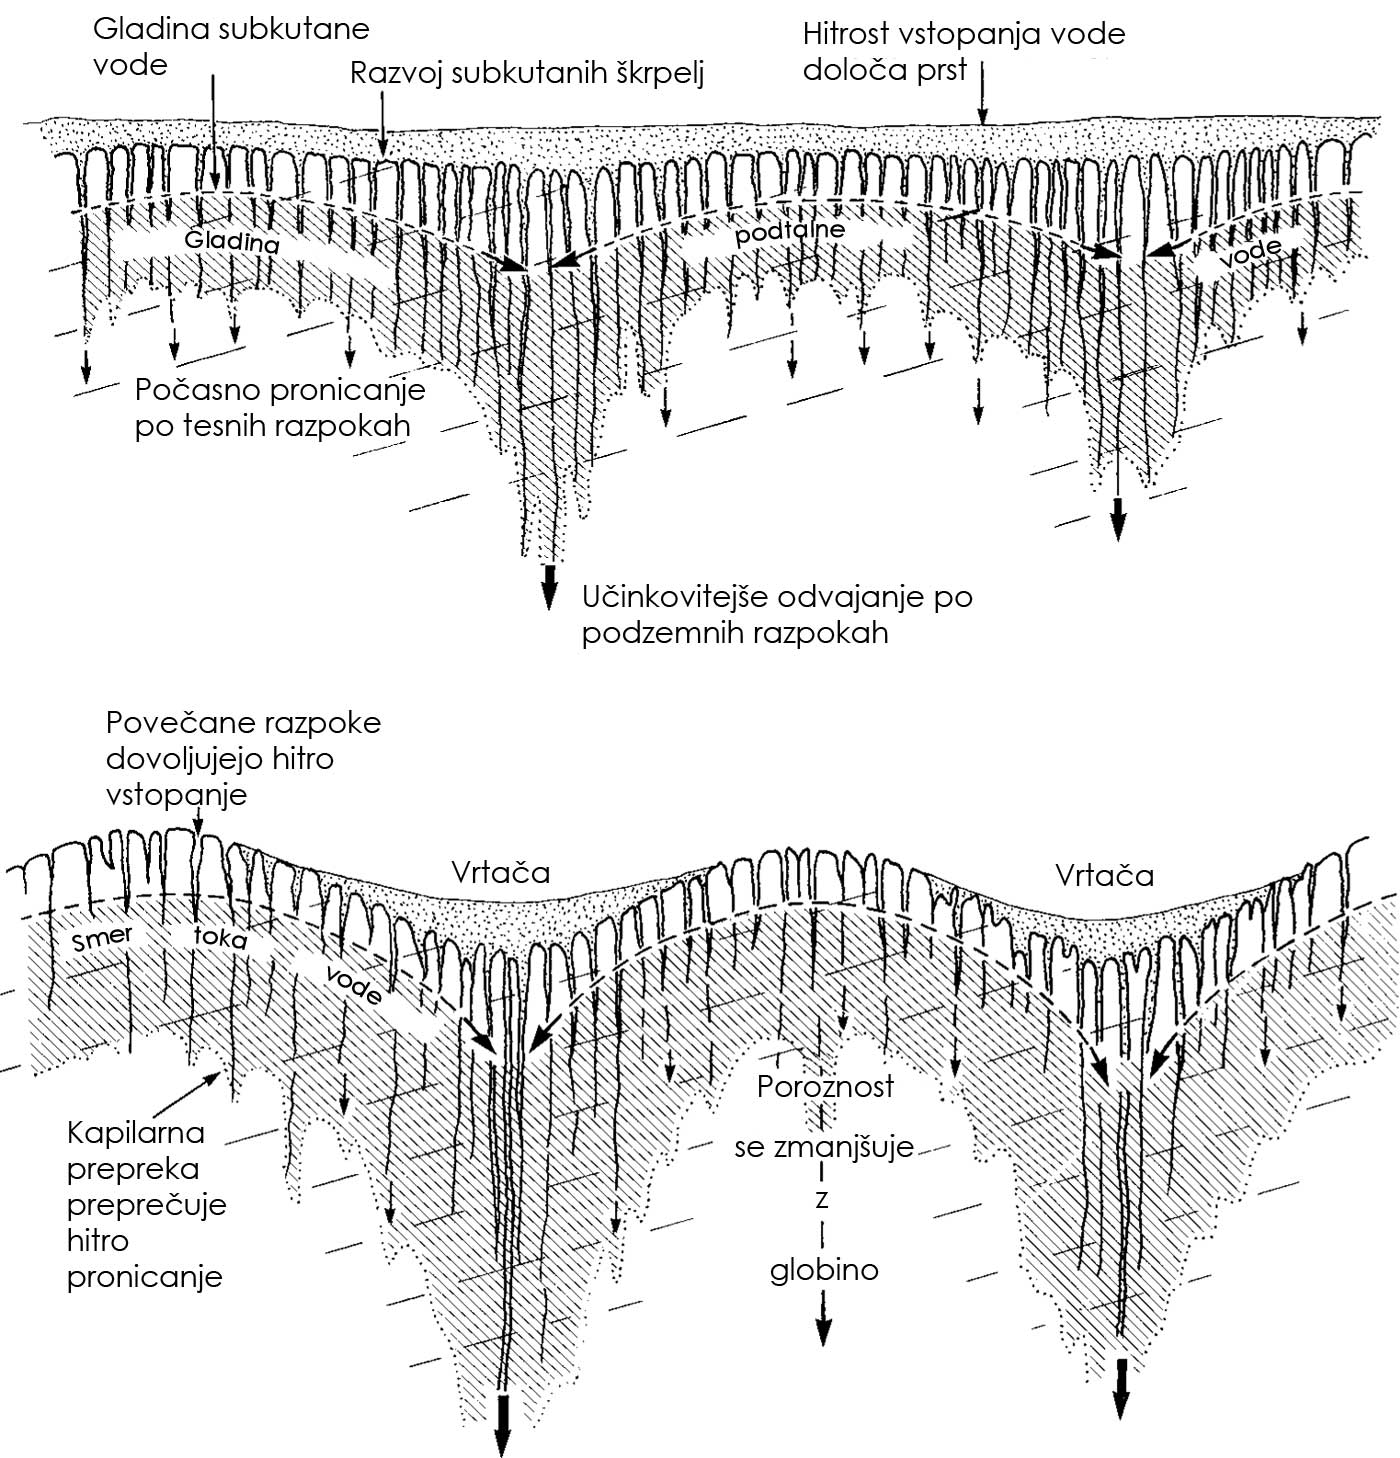
\includegraphics[width=7.5cm]{slike/vrtaca-ford-williams.jpg}
  \end{center}
  \caption{Geomorfološka skica nastanka vrtač. Na sprva ravnem površju neka začetna točka malenkost bolje odvaja vodo v podzemlje. Zaradi večjega pretoka vode se tam na stiku prsti in kamnine poveča raztapljanje apnenca. Raztapljanje in odnašanje apnenca v podtalnico poglobi površje in s tem poveča lokalno povodje in s tem količino vode odvajane v začetno točko. Dobimo pozitivno povratno zanko in oblikujejo se vrtače. S časom se v vrtačah nabere slabše prepustna prst, odvajanje vode skozi večje razpoke se izboljša, raztapljanje na dnu vrtače zmanjša. To deluje kot negativna povratna zanka. Vir: \cite{ford2007karst}.}
\label{fig:vrtaca-ford-williams}
\end{figure}

Na ta model se bomo oprli, ko bomo poskusili modelirati dinamiko vrtač.

  Za študij realnih vrtač uporabimo z LiDARjem pridobljen digitalni model reliefa Menišije (Slika \ref{fig:menisija-karta}) ločljivosti 1m, ki nam da natančno višinsko karto velike količine vrtač, ter omogoči zanesljivo identifikacijo in študij tega pojava (Slika \ref{fig:menisija-relief}).

  LiDAR je okrajšava za Light Detection And Ranging. Pri LiDARskih meritvi relief preleti letalo, ki s pomočjo GPSa, žiroskopov in akcelerometrov natančno spremlja svojo lokacijo in orientacijo v prostoru, ter hkrati meri odbojni čas laserskega žarka, s katerim prečesava relief pravokotno na smer svojega leta. Iz odbojnih časov in lokacije letala nato izračunamo oblak višinskih točk, ki vključujejo točke na tleh, drevesih, umetnih objektih, itn. Komercialni LiDARji delujejo do višine 5000m in zajamejo $5 \cdot 10^5$točk/sekundo. Višinska natančnost meritev je nekaj centimetrov, en prelet pa tipično posname pas širine enega kilometra. Rezultat je oblak višinski točk z gostoto od 1 do 10 točk $/ m^2$.

  Ker je Menišija z gozdom poraščeno območje, je Geodetski inštitut Slovenije, ki je meritve pridobil, iz oblaka višinskih točk po metodi REIN \cite{Kobler20079} odfiltriral višinske točke dreves in ostalega rastja. Metoda REIN (REpetetive INterpolation) z naključnim vzorčenjem oblaka višinskih točk interpolira površje in na podlagi interpoliranega površja izbere in zavrže osamele točke oblaka točk.

  \begin{figure}[h]
    \begin{center}
      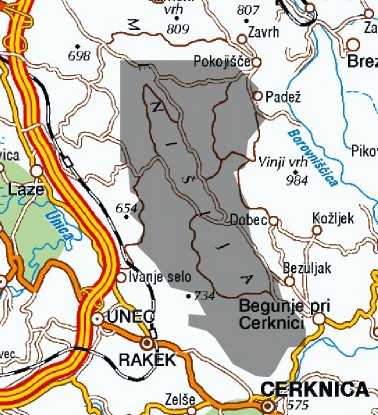
\includegraphics[width=7cm]{slike/menisija-karta}
    \end{center}
    \caption{Menišija, $60 km^2$ veliko območje med Cerknico in Logatcem, vsebuje nekaj tisoč vrtač ter nekaj udornic in predstavlja približno odstotek slovenskega krasa. Osenčen del zemljevida označuje področje digitalnega modela reliefa uporabljenega v tej nalogi (Slika \ref{fig:menisija-relief}). Vira: Geopedia, Geodetski inštitut Slovenije.}
    \label{fig:menisija-karta}
  \end{figure}

  Površje Menišije sestavljajo plasti krednega apnenca (starost nastanka 135-65 milijonov let), ki so bili zaradi dogodkov, povezanih s podrivanjem Adriatske plošče v Miocenu (17-7 milijonov let) prišli na površje. Območje Menišije je bilo do 3.5 milijona let pred sedanjostjo s poplavami uravnavano kraško polje, nato pa se je zaradi tektonske aktivnosti dvignilo nad okolico. S tem se je uravnavanje prenehalo in vzpostavljeni so bili geomorfološki pogoji za nastanek vrtač.

Hitrost zniževanja (denudacije) kraškega površja zaradi kemičnega preperevanja apnenca, se ocenjuje na 20-50 m / milijon let, torej se je površje Menišije v času od prenehanja uravnavanja znižalo za 70-175m, hkrati pa so se v njem pojavile vrtače, udornice in brezstrope jame. \cite{Vrabec2006} \cite{Placer2010}

Denudacijo kraškega površja povzroča kemična erozija apnenca. Apnenec raztaplja šibka ogljikova kislina, ki nastane z raztapljanjem ogljikovega dioksida v vodi. Na mestih, kjer se voda ne more zadrževati, na primer na goli skali, je denudacija počasnejša, oblikujejo se škraplje in žlebiči velikosti od nekaj milimetrov do nekaj metrov. Kraška polja, velikosti od deset do sto km, ki so pogosto poplavljena, pa denudacija uravna.

Iz geologije torej izvemo, da se je uravnano površje Menišije v obdobju 3.5 milijonih let zaradi raztapljanja kamnine stalno zniževalo, hkrati pa se je na njem pojavilo veliko število vrtač.

Vrtače take velikosti in oblike najdemo tudi v drugih delih Dinarskega krasa. Na teh področjih so bili pogoji za nastanek vrtač zaradi drugačne geološke dinamike lahko vzpostavljeni prej ali kasneje kot v Menišiji. Poleg tega na nastanek vrtač vplivajo še lokalni dejavniki: kemična sestava in kot vpadanja plasti apnenca, nadmorska višina, parcialni tlak ogljikovega dioksida, količina padavin, temperatura in biološki dejavniki. Oblika in velikost vrtač je kljub lokalnim variiacijam univerzalna po celotnem Dinarskem krasu.

Iz tega sklepamo, da se bodo pri določenih pogojih na ravnem kraškem površju sčasoma neizogibno oblikovale vrtače. Če so vrtače, po dolgem času, podobnih si dimenzij, sklepamo da konvergirajo proti stabilni univerzalni obliki, ki je po dolgem času neodvisna od lokalnih detajlov.

Da dinamiko vrtač bolje osvetlimo, bomo v (Poglavje \ref{realne-vrtace}) pregledali velik vzorec vrtač, ki nam ga nudi LiDARski posnetek Menišije in poročali kakšne vrtače tam najdemo. Nato bomo v (Poglavje \ref{analiticno-modeliranje}) dobljeni povprečni vrtači poskusili z različnimi prijemi pripisati časovno dinamiko.

 \begin{figure}[h!]
    \begin{center}
      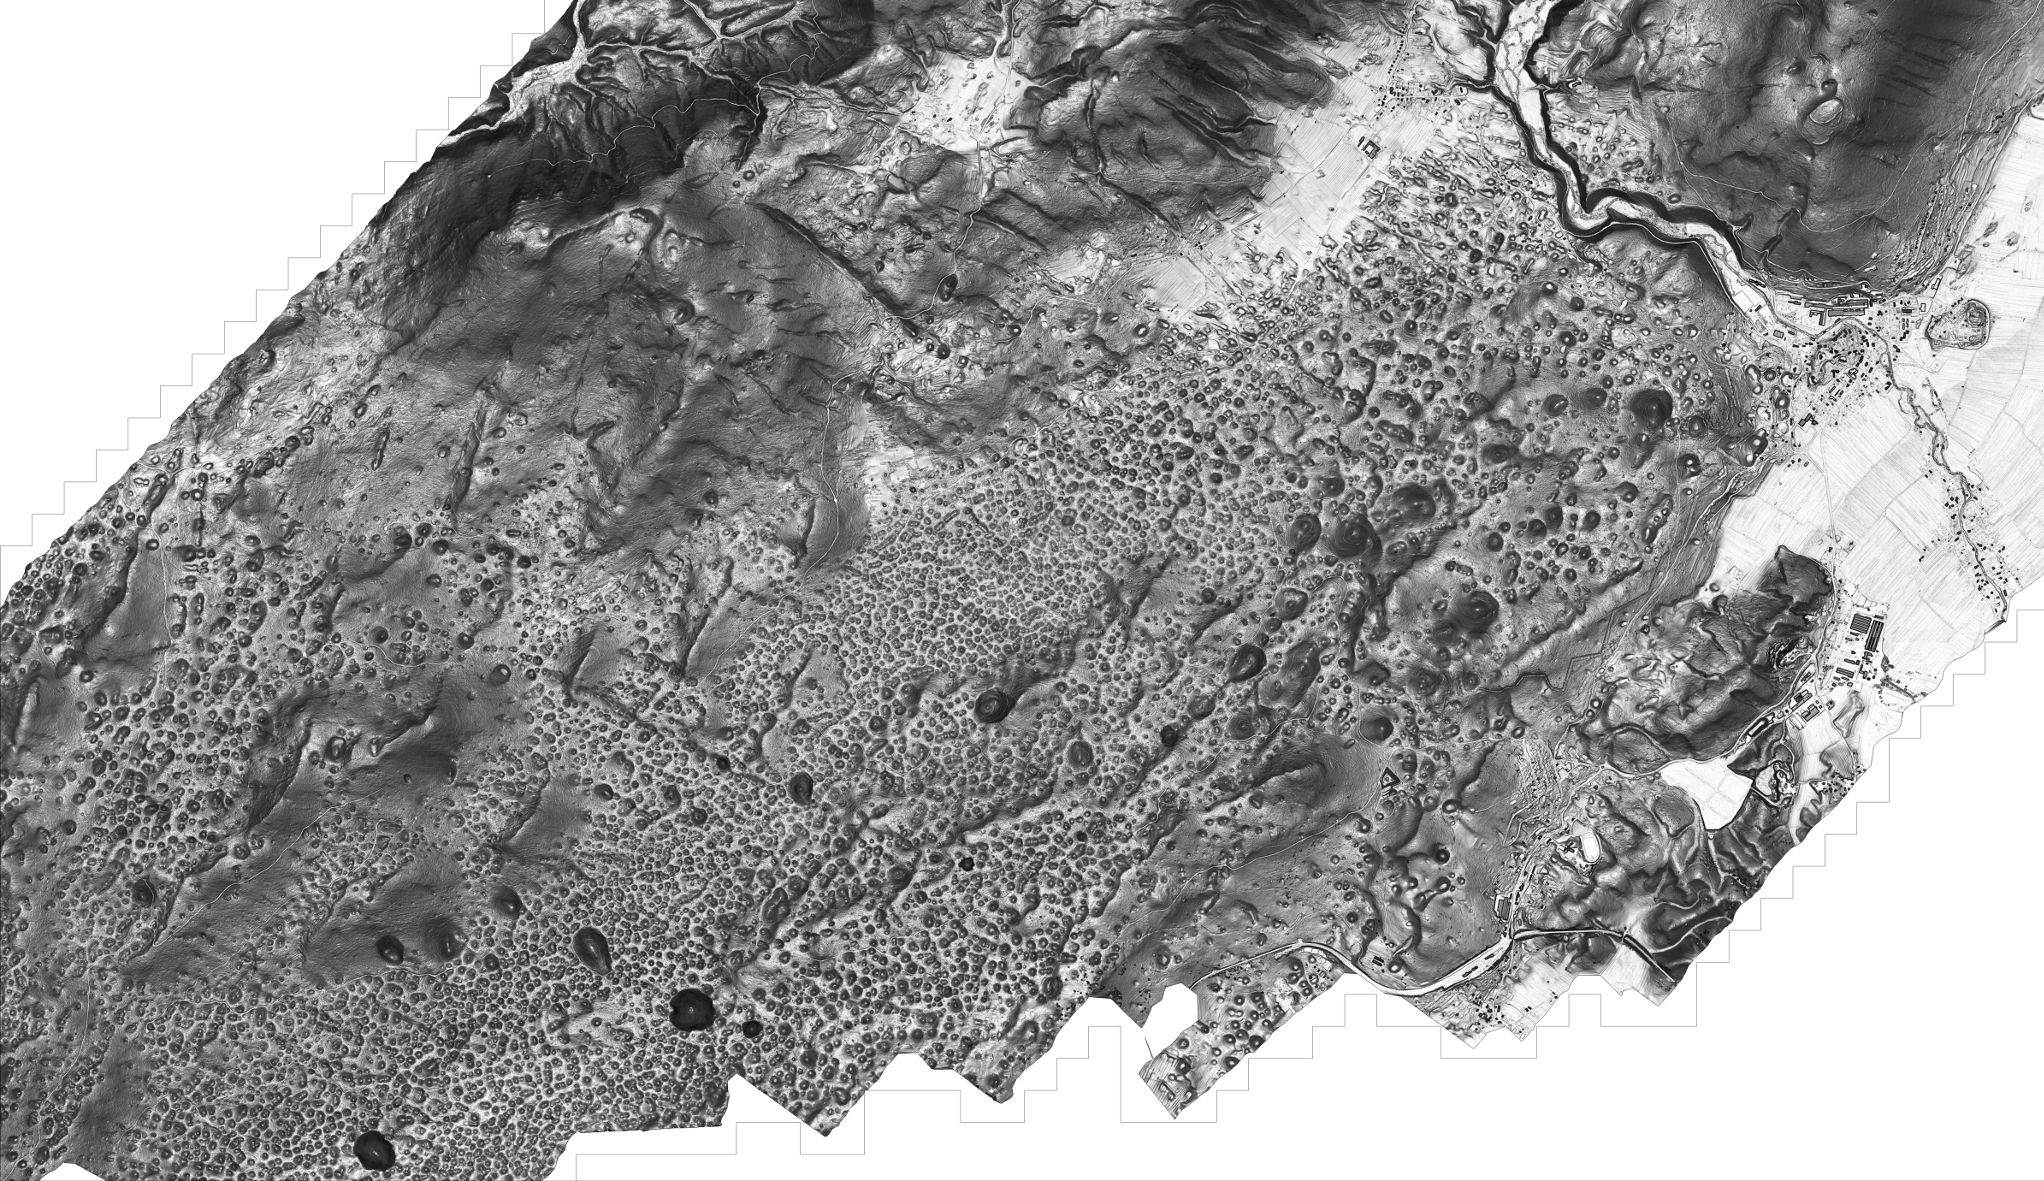
\includegraphics[width=8.5cm]{slike/menisija-relief}
    \end{center}
    \caption{Senčen digitalni model reliefa dela Menišije uporabljen v tej nalogi. Vir: Geodetski inštitut Slovenije \cite{LAK} po metodi REIN \cite{Kobler20079}.}
    \label{fig:menisija-relief}
  \end{figure} 

  \chapter{Realne vrtače}
  \label{realne-vrtace}

V tem poglavju bomo iz celotnega LiDARskega posnetka Menišije (Slika \ref{fig:menisija-relief}) z digitalnim algoritmom izbrali kraške vrtače in predlagali funkcijo, ki jih v povprečju opiše. Nato bomo to funkcijo prilegali na posamezne vrtače in komentirali porazdelitev parametrov funkcije.

  \section{Segmentacija vrtač}

Identifikacijo velike količine objektov se lotimo s segmentacijo po indeksu konkavnosti, kot predlaga \cite{doctor13}. Uvedemo lokalni indeks konkavnosti $I_k$ (\ref{ik}), ki ga izračunamo tako, da od izbrane točke v matriki višinskih točk odštejemo povprečno vrednost točk, izbrani točki koncentričnega kolobarja:
\begin{equation}  I_k(r_0,r_1,r_2) = h(r_0)- \frac{1}{N}\sum\limits_{r_1<r<r_2} h(r). \label{ik} \end{equation}

  \begin{figure}[h!]
    \begin{center}
      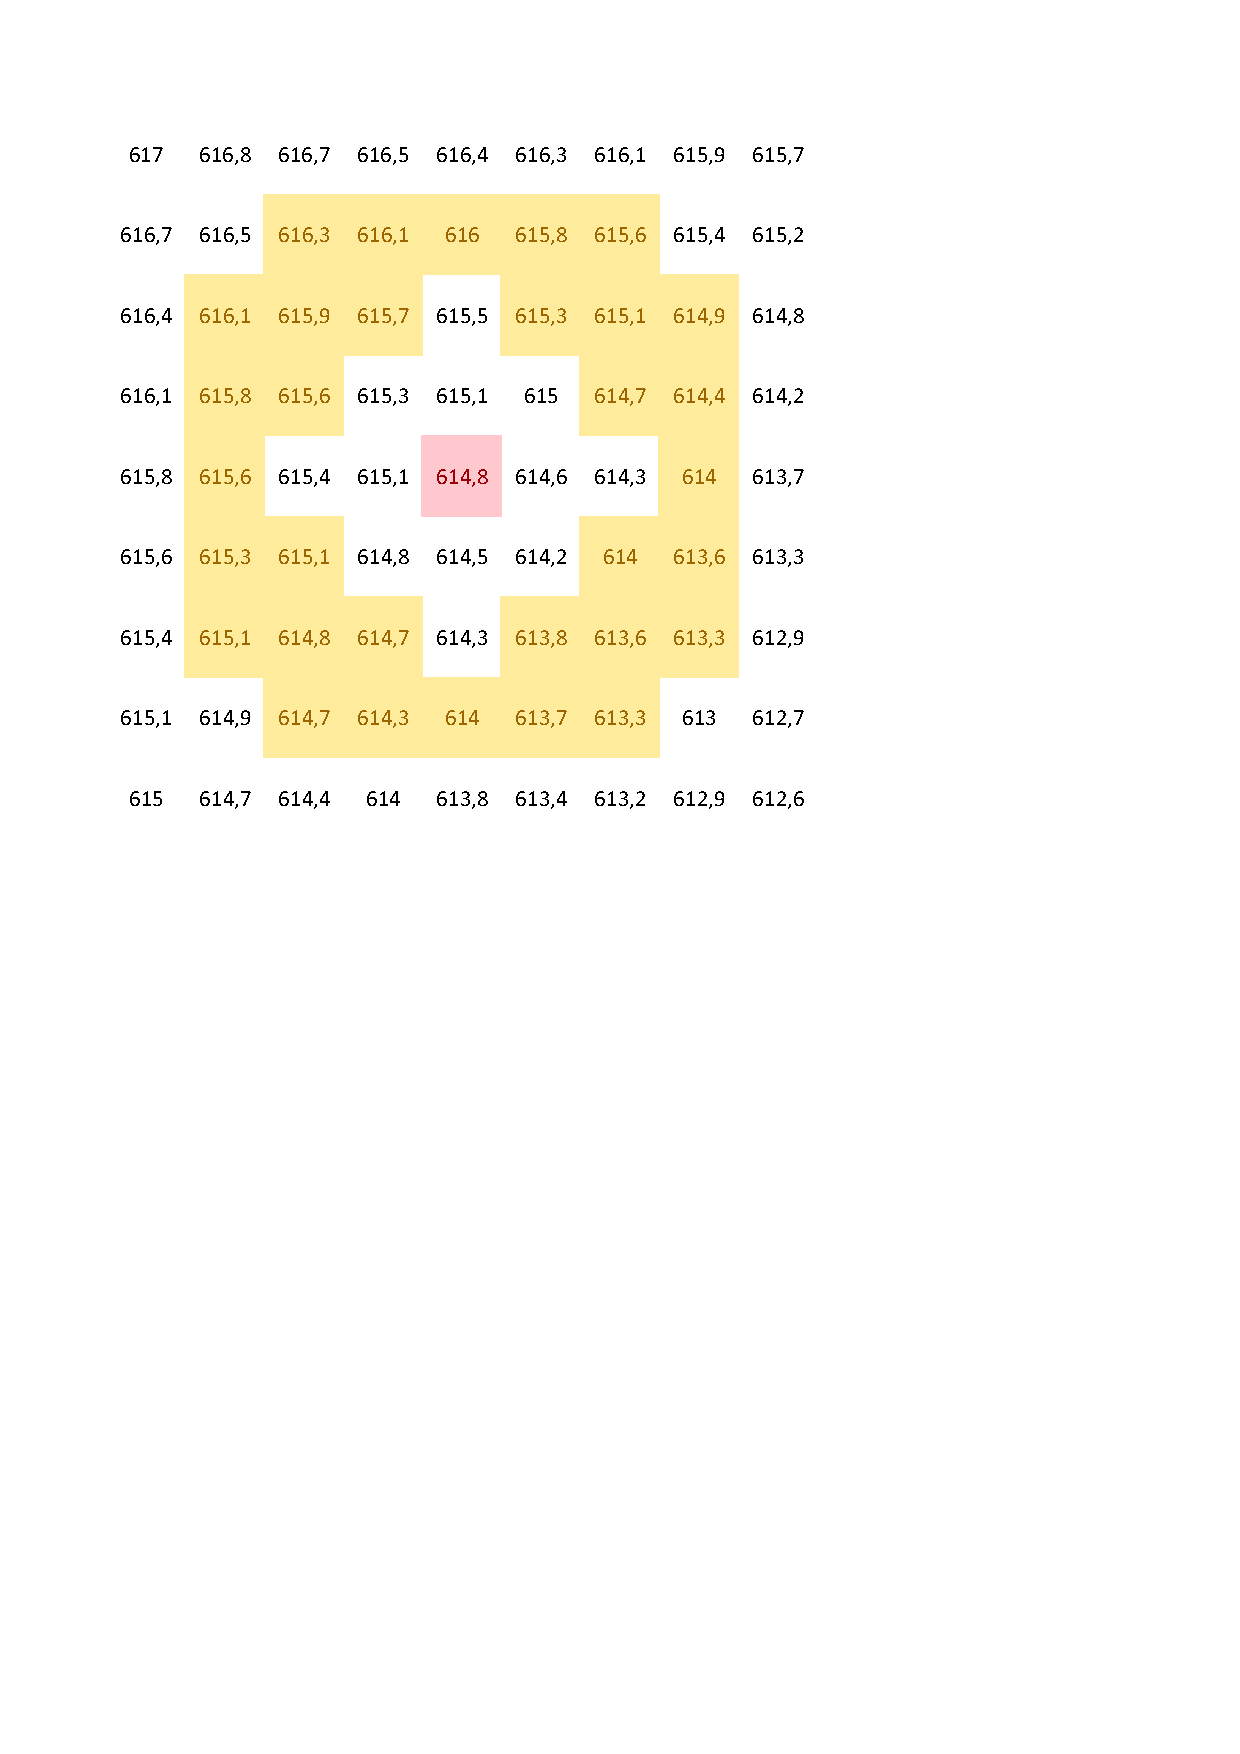
\includegraphics[width=4cm]{slike/concavity-ring-visualisation-2}
    \end{center}
    \caption{V prikazanem primeru je indeks konkavnosti, $I_k = 614,8 - 19676,2/32 = - 8,125 \cdot 10^{-2}$.}
    \label{fig:concavity-ring}
  \end{figure}

Center kolobarja postavimo v točko katere indeks konkavnosti računamo, $r_1$ in $r_2$ pa sta notranji ter zunanji radij kolobarja.
Primer kolobarja vidimo na (Slika \ref{fig:concavity-ring}). Indeks konkavnosti izračunan na konkavni ploskvi bo negativen, na konveksni pa pozitiven. Če ima ploskev konkavna in konveksna področja, bo rezultat odvisen tudi od izbire okolice.

Postopek ponovimo po celotni matriki višinskih točk. Rezultat je matrika indeksa konkavnosti.

Tudi od dimenzij, ki jih izberemo za kolobar je odvisno, ali bodo določene točke v reliefu imele pozitven ali negativen indeks konkavnosti. Empirično se odločimo za tri kolobarje različnih velikosti $(r_1=10,r_2=15;r_1=15,r_2=25;r_1=60,r_2=100)$, za katere ocenimo da z njimi najdemo največ vrtač. Z njimi izračunamo indeks konkavnosti, ki je prikazan na (Slika \ref{fig:concavity-samples}). Večji kot je kolobar, bolj izpovprečen je indeks konkavnosti.

  \begin{figure}[h!]
    \begin{center}
      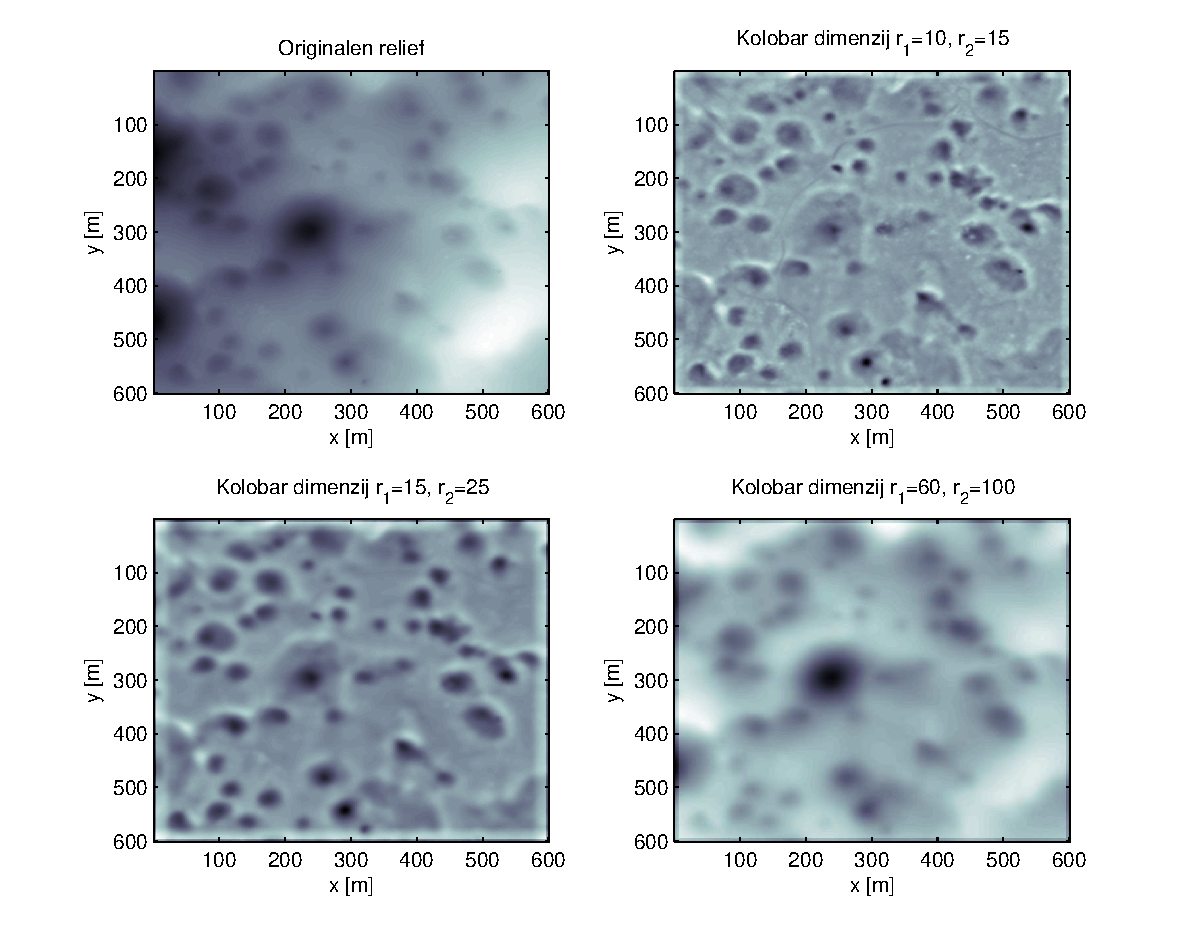
\includegraphics[width=12cm]{slike/concavity-samples}
    \end{center}
    \caption{Indeks konkavnosti reliefa $I_k$ definiranega v (\ref{ik}), pri različno izbranih dimenzijah kolobarja $(r_1=10,r_2=15;r_1=15,r_2=25;r_1=60,r_2=100)$.}
    \label{fig:concavity-samples}
  \end{figure}

Izračunamo standardno deviacijo indeksa konkavnosti $\sigma_{I_k}$. Arbitrarno odločimo, da so konveksni tisti deli površja (svetlejši odtenki), kjer je $I_k > -\frac{\sigma_{I_k}}{2}$. Zavržemo jih in konkavne (temnejši odtenki) dele površja odberemo kot vrtače. Vidimo, da pri izbiri manjšega kolobarja najdemo več vrtač, a podcenimo njihovo velikost. Pri izbiri večjega kolobarja pa se zgodi, da več manjših vrtač prepoznamo kot eno veliko. Zato vse tri rezultate primerjamo in v primeru, da večja vrtača prekriva eno manjšo, izberemo večjo vrtačo in zavržemo manjšo. V primeru da velika vrtača prekrije več manjših izberemo manjše. Rezultat je segmentacija vrtač na (Slika \ref{fig:concavity-segmentation-samples}).
  \begin{figure}[h!]
    \begin{center}
      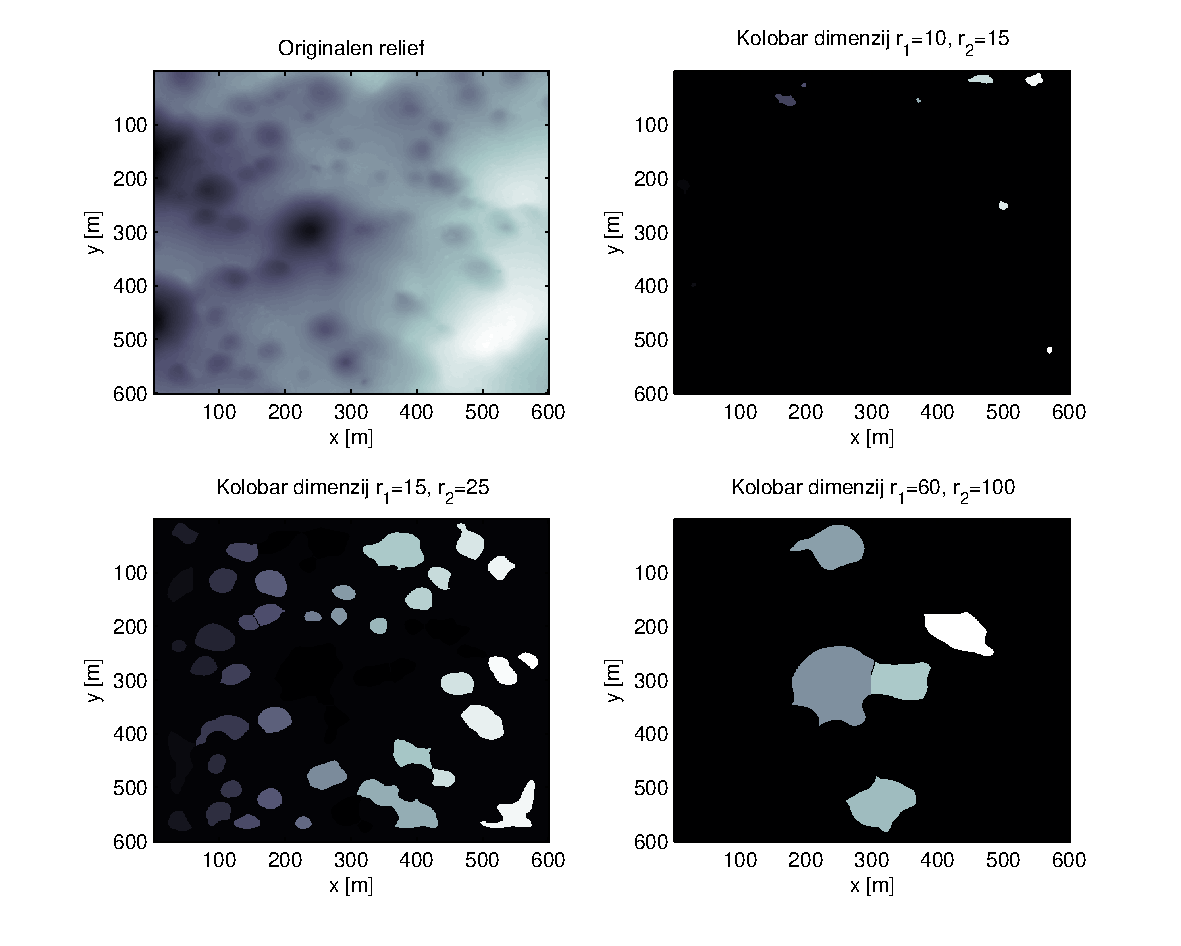
\includegraphics[width=12cm]{slike/concavity-segmentation-samples.pdf}
    \end{center}
    \caption{Indeks konkavnosti reliefa $I_k$ definiranega v (\ref{ik}), pri različno izbranih dimenzijah kolobarja $(r_1=10,r_2=15;r_1=15,r_2=25;r_1=60,r_2=100)$.}
    \label{fig:concavity-segmentation-samples}
  \end{figure}

Sedaj vrtače zarišemo preko večjega senčenega reliefa: (Slika \ref{fig:menisija-vrtace}). Na sliki opazimo tudi, da kljub trudu nekoliko podcenimo velikost vrtač, saj niso obkrožene točno po robu, ampak nekoliko znotraj njihovega zunanjega oboda. Za statistično analizo to ni moteče, saj podcenitev napravimo na vseh vrtačah in na enak način.
  \begin{figure}[h]
    \begin{center}
      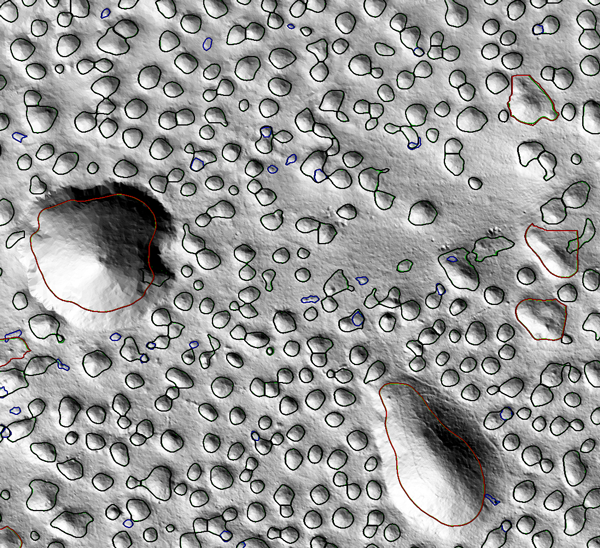
\includegraphics[width=7cm]{slike/menisija-vrtace}
    \end{center}
    \caption{Del od 8687 zaznanih vrtač na območju Menišije. Poleg vrtač so na sliki vidni tudi dve udornici, ki so velikostni red večje in imajo ostrejši rob kot vrtače. Vrtače, ki smo jih zaznali pri izbiri manjšega kolobarja so obkrožene z modro barvo, vrtače srednjega kolobarja z črno in vrtače velikega z rdečo. Pri udornicah je posebno opazna podcenitev velikosti.}
    \label{fig:menisija-vrtace}
  \end{figure}

Z ročnim pregledom celotnega reliefa preverimo, da je večina najdenih objektov res vrtač.

  \section{Analiza}

  Površino vrtač definiramo s številom višinskih točk (pikslov), ki jo sestavljajo:
    \begin{equation}
      A = \sum pikslov.
    \end{equation}

S to količino nato definiramo efektivni polmer objektov:
    \begin{equation} 
      r_{eff} = \sqrt{\frac{A}{\pi}}. 
    \end{equation}

Zaradi oblike histograma efektivnih polmerov (Slika \ref{fig:menisija-polmeri-hist}) se zdi smiselno, da ga prilegamo k Maxwellovi podobni porazdelitvi, čeprav za to nimamo globljih teoretičnih argumentov:
\begin{equation} 
  N(r_{eff}) = A r_{eff}^2 e^{-(r_{eff}/ 2 \sigma_{eff})^{\alpha}},
\end{equation}
dobimo rezultat $\sigma_{eff}=12m$, $A=0,24m$ in $\alpha=2,5$. Povprečen efektivni polmer objekta je $\bar r_{eff}=26m$.

  \begin{figure}[h!]
    \begin{center}
      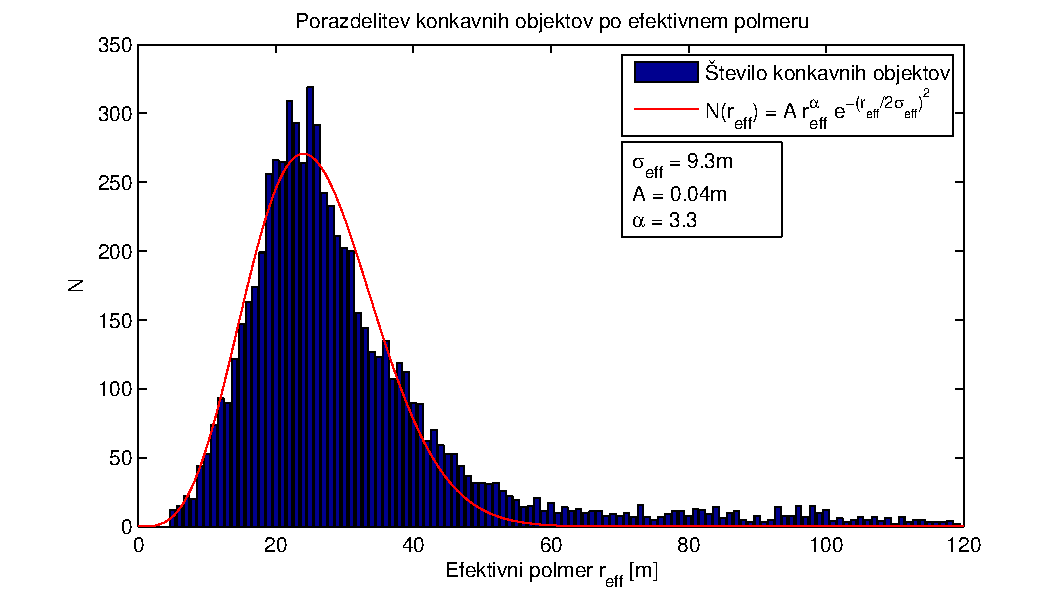
\includegraphics[width=12cm]{slike/menisija-polmeri-hist-maxwell}
    \end{center}
    \caption{Histogram efektivnih polmerov konkavnih objektov v Menišiji. Povprečen efektivni polmer objekta je $\bar r_{eff}=26m$, prilegana Maxwellovi podobna porazdelitev: $ N = A r_{eff}^{\alpha} e^{-(r_{eff}/2 \sigma_{reff})^{\alpha}}$, pa ima parametre $\sigma_{eff}=12m$, $A=0,24m$ in $\alpha=2,5$}
    \label{fig:menisija-polmeri-hist}
  \end{figure}

  Posamezne realne vrtače zaradi lokalnih pogojev in zgodovine razvoja reliefa niso simetrične, a zdi se, da so si med seboj podobne. Da bi ugotovili statistično najverjetnejšo obliko vrtače, izračunamo povprečje velikega števila realnih vrtač. Uporabimo dva pristopa. Pri prvem vrtače različnih velikosti z najmanjšim možnim kvadratom objamemo in izrežemo, nato jih vse raztegnemo na isto velikost in povprečimo. Dobimo (Slika \ref{fig:menisija-vrtaca}). Pri drugem pristopu pa vrtače razdelimo v pet velikostnih razredov (20\% najmanjših gre v prvi razred, itn.) in jih znotraj razredov povprečimo, a jih za razliko od prvega pristopa ne raztegnemo. Dobimo (Slika \ref{fig:menisija-vrtace-po-razredih}).

  \begin{figure}[h!]
    \begin{center}
      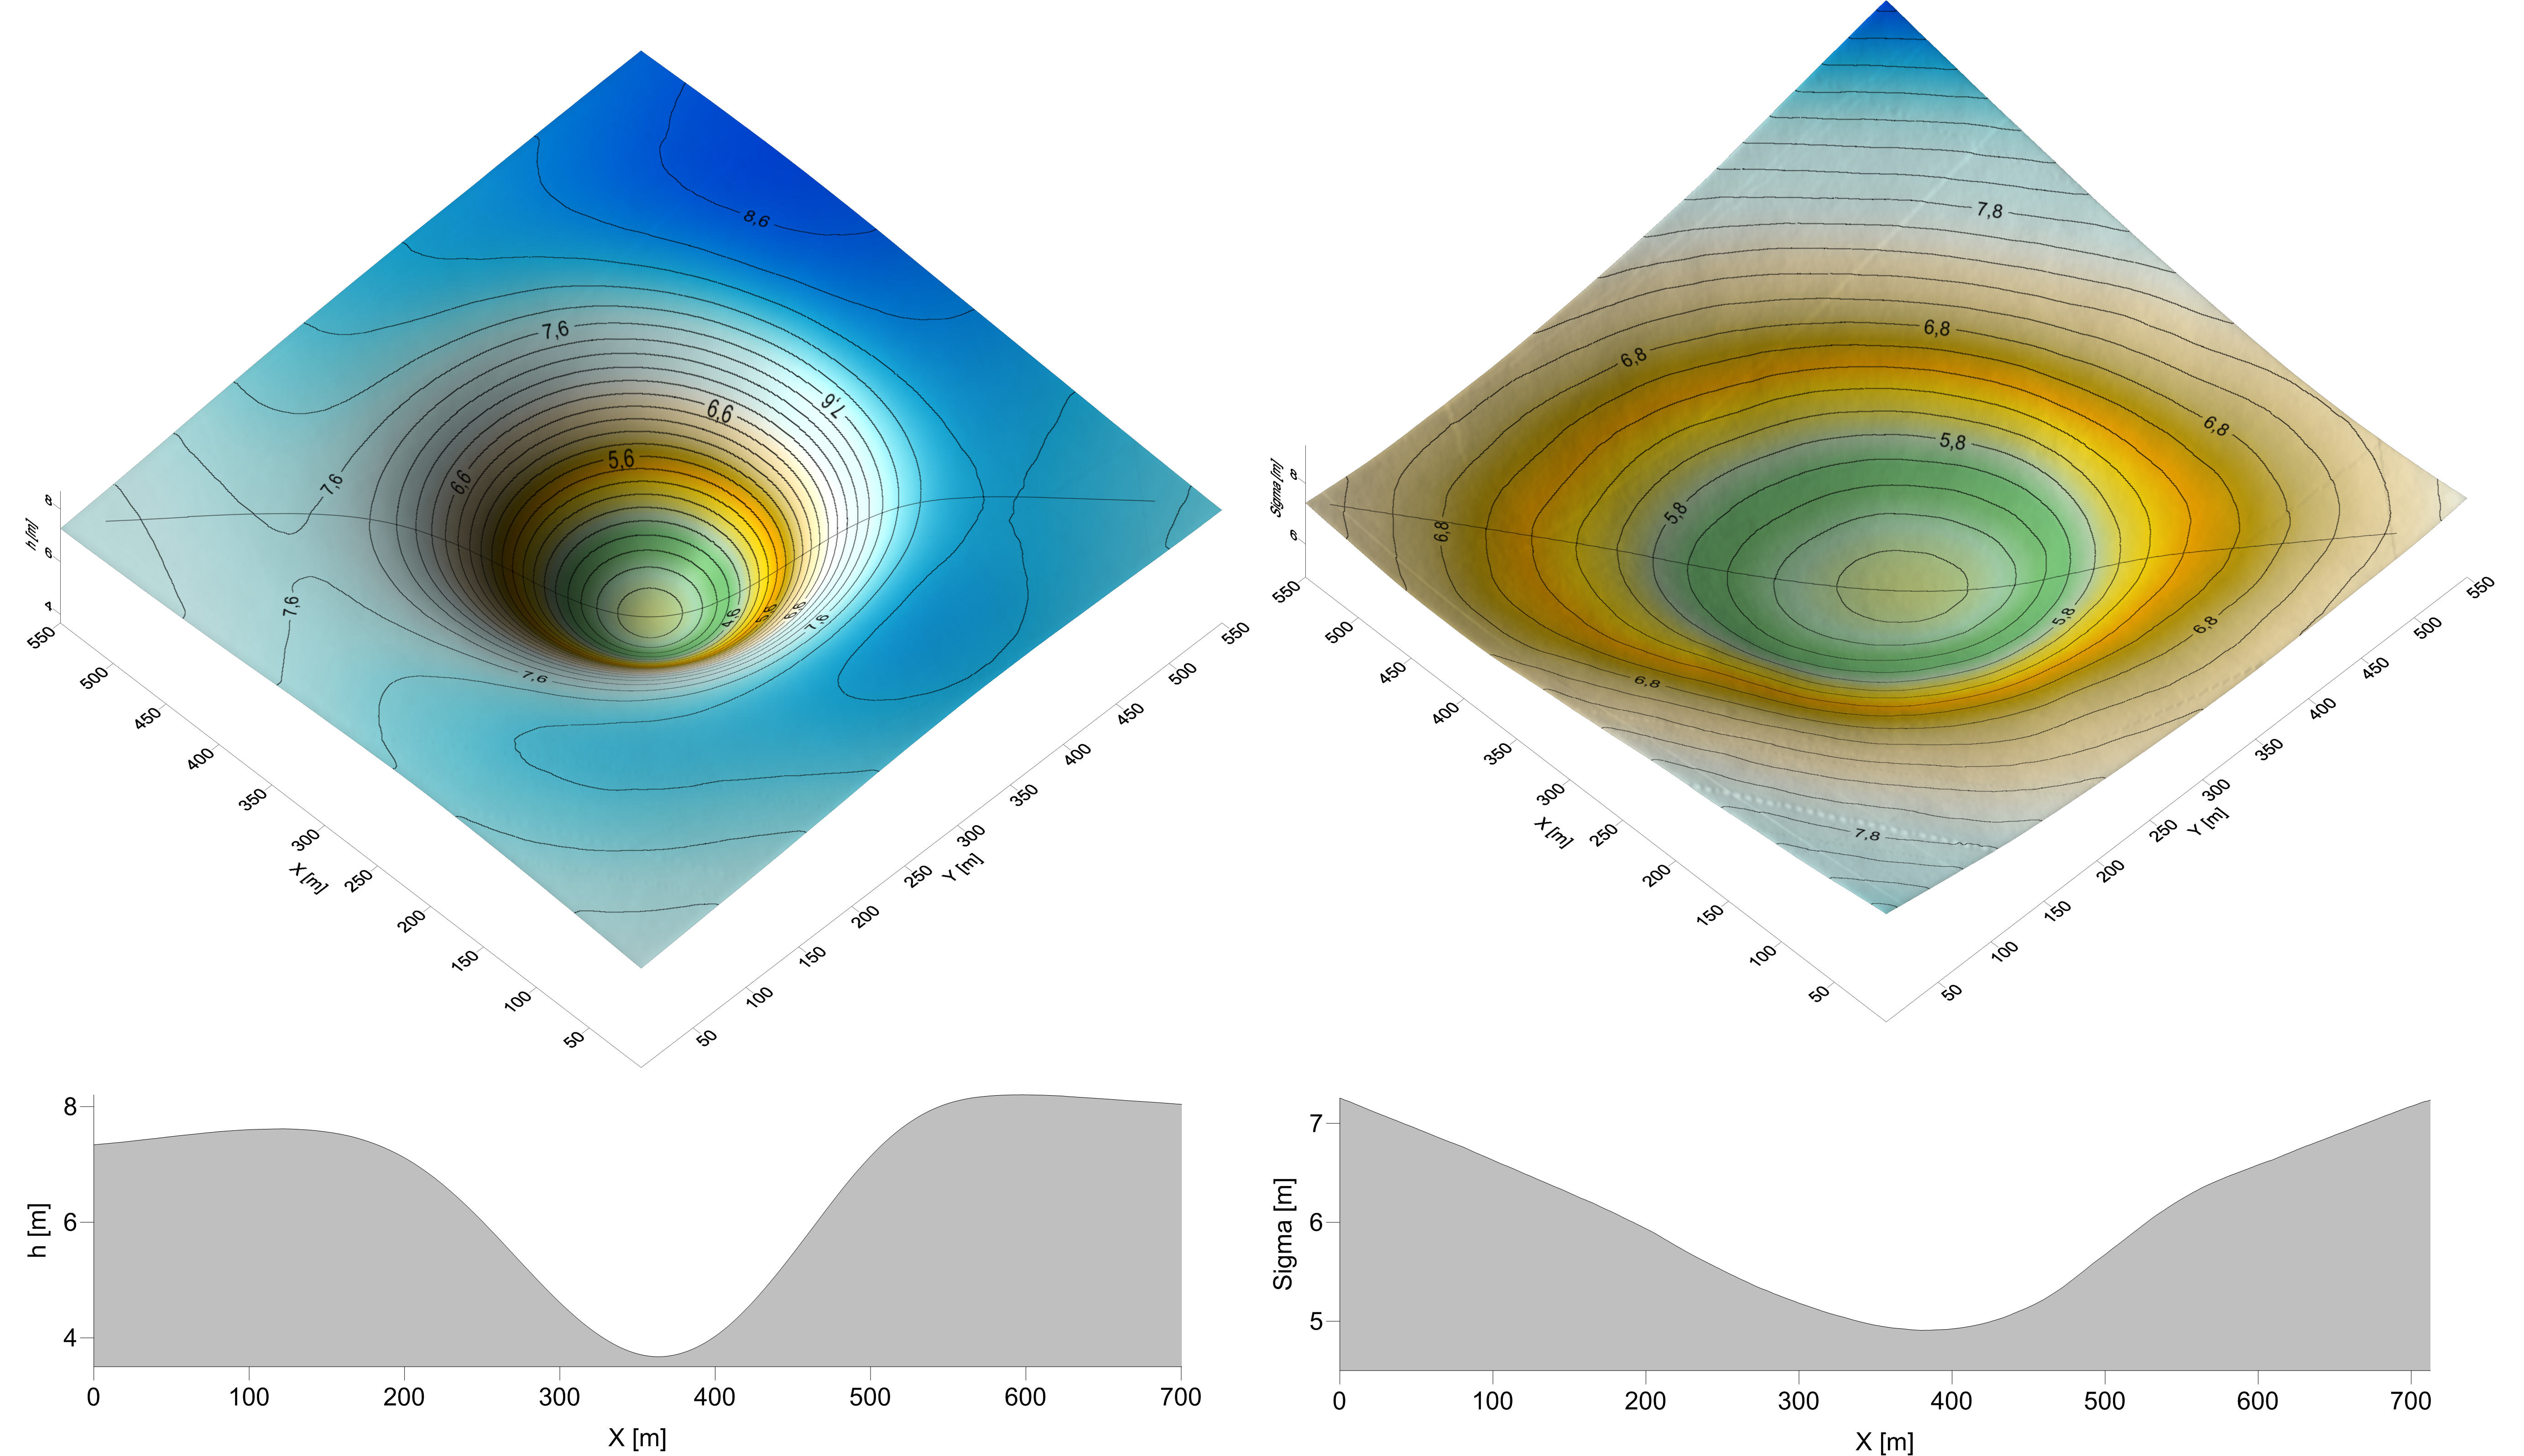
\includegraphics[width=14cm]{slike/menisija-vrtaca-sigma}
    \end{center}
    \caption{Levo: povprečje 8687 realnih vrtač z območja Menišije, pred povprečjem so bile vrtače raztegnjene na velikost največje v setu. Desno: standardna deviacija istega seta vrtač od povprečja.}
    \label{fig:menisija-vrtaca}
  \end{figure}

  \begin{figure}[h!]
    \begin{center}
      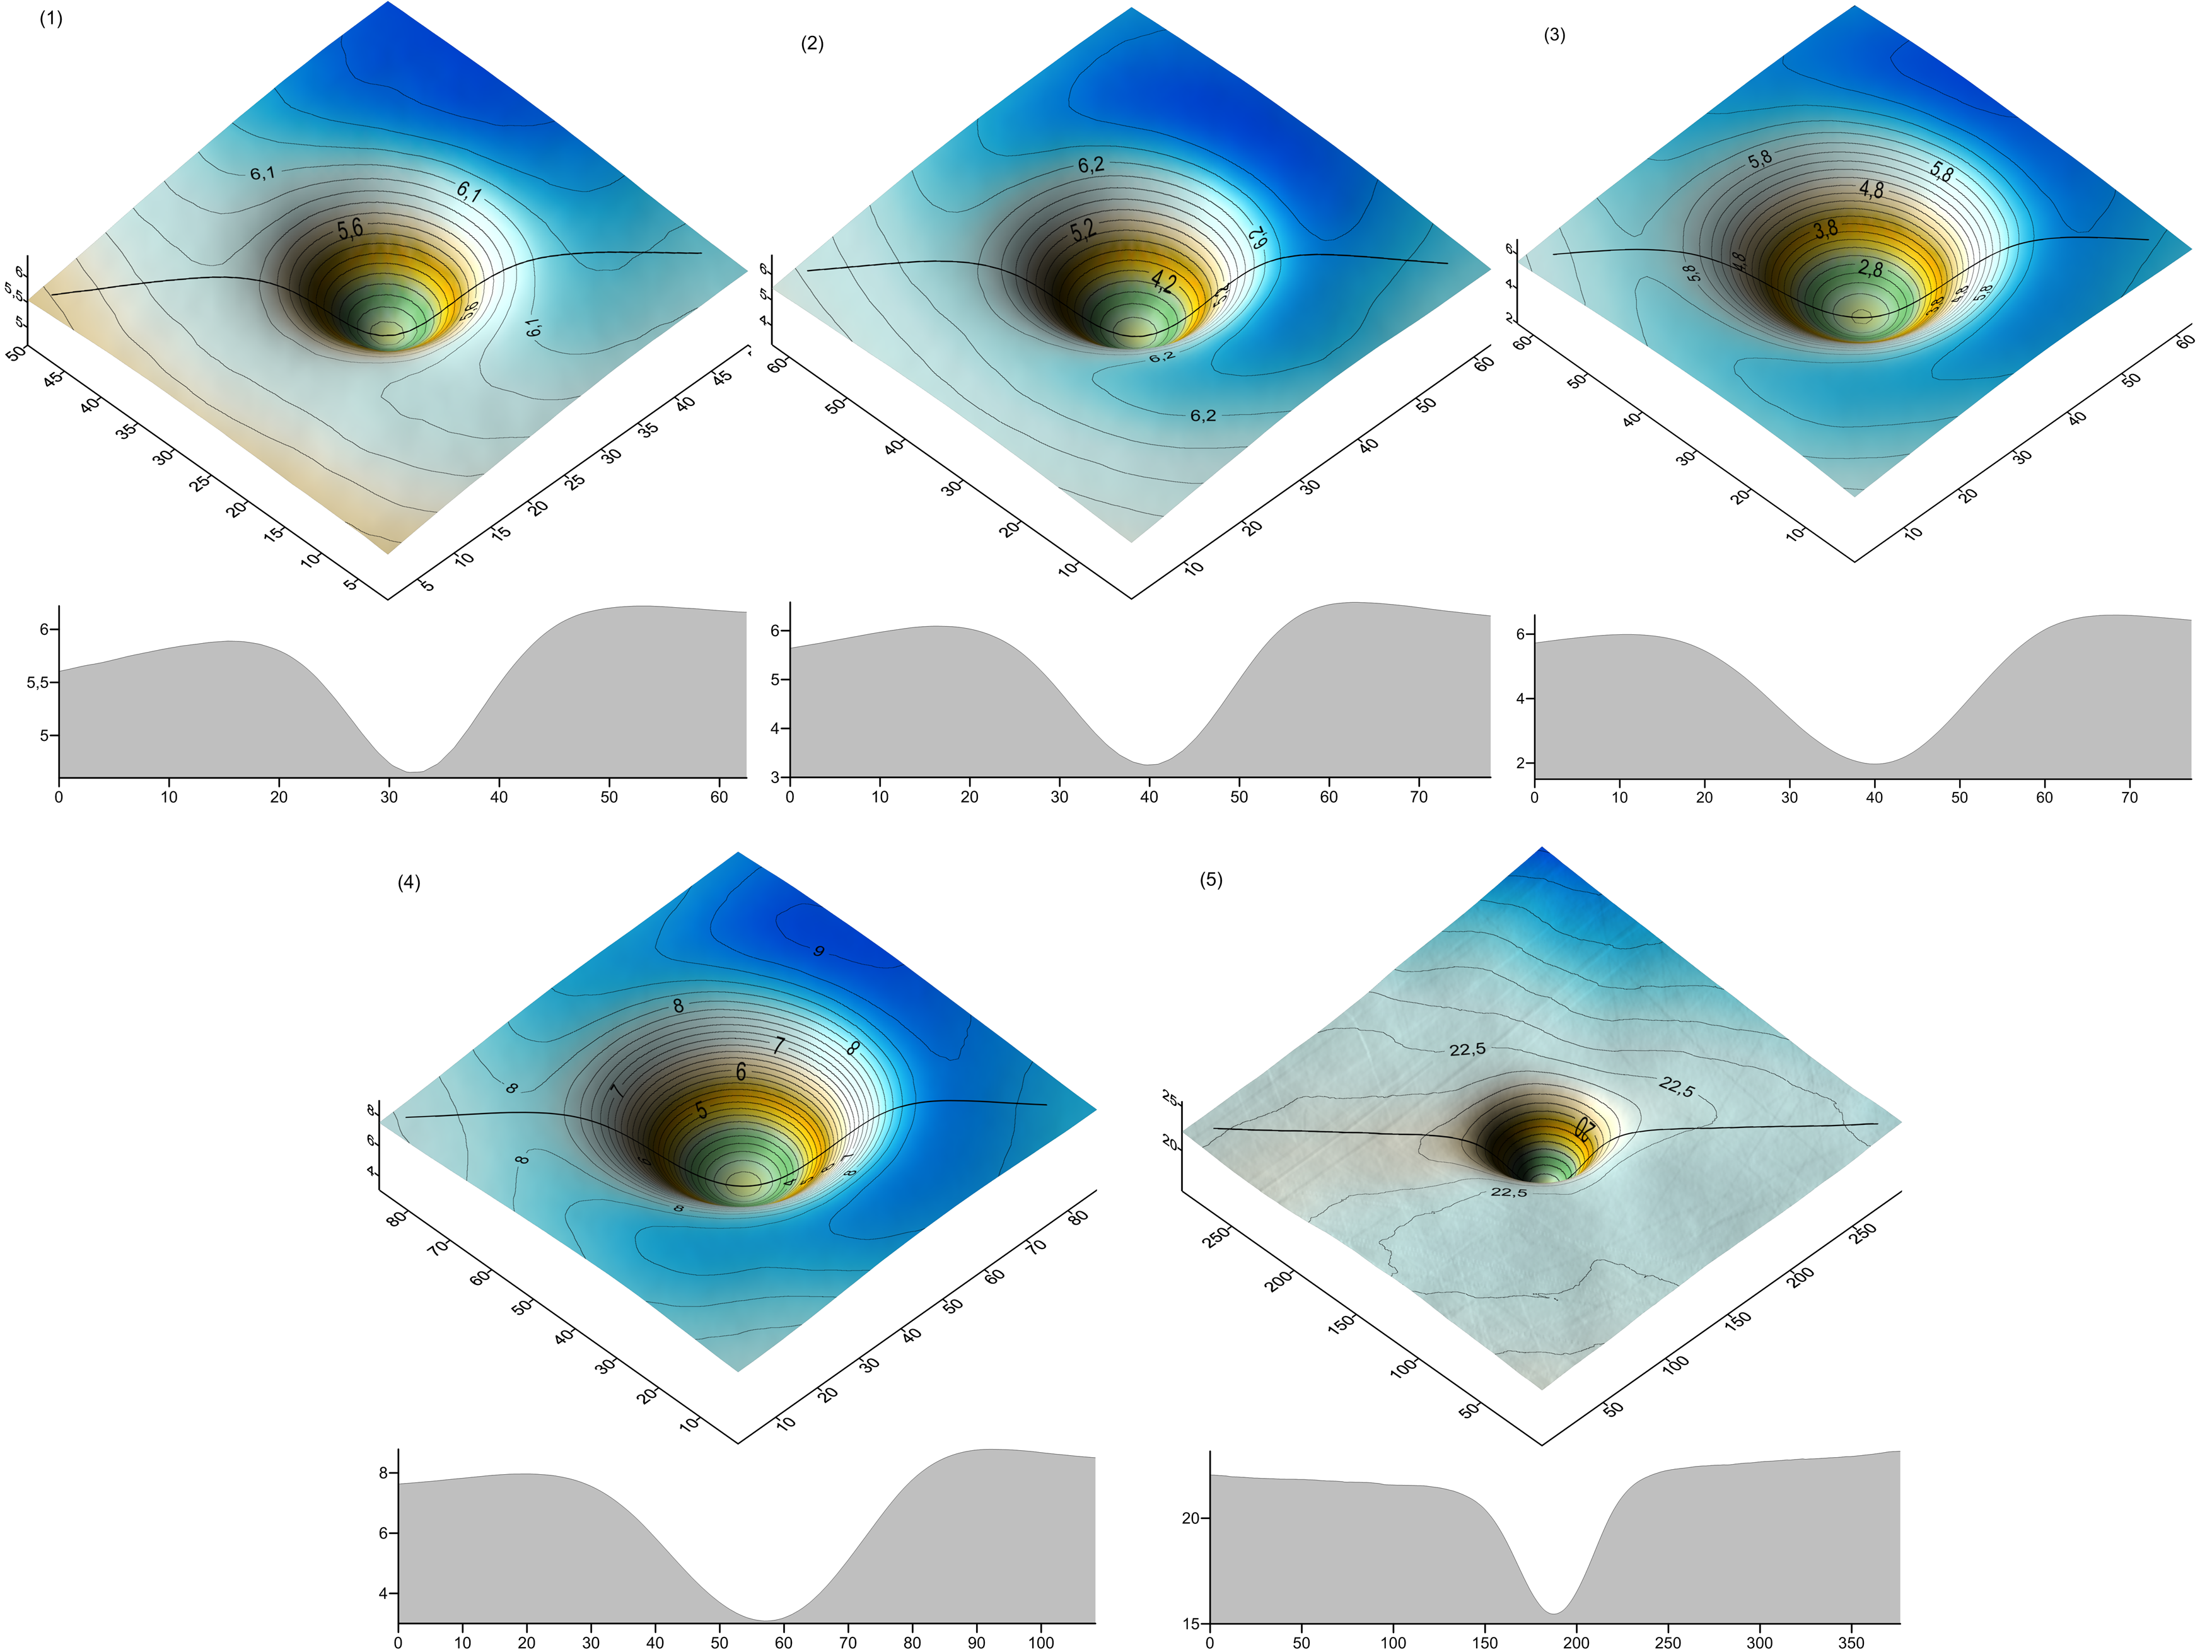
\includegraphics[width=15cm,angle=90]{slike/vrtace-po-razredih-menisija}
    \end{center}
    \caption{Vrtače po velikosti razdelimo v pet razredov (najmanjša petina gre v prvi razred, itn.). Vrtače znotraj razreda tako izrežemo iz površja, da je matrika višinskih točk vrtače vedno enakih dimenzij, pri čemer se vrtača nahaja v sredini. Set vrtač znotraj razredov povprečimo in izrišemo. Dobljeni rezultati so podobni rezultatom povprečenja, pri katerih smo vse vrtače raztegnili na velikost največje v setu: (\ref{fig:menisija-vrtaca}), kar nam da več zaupanja v oba rezultata.}
    \label{fig:menisija-vrtace-po-razredih}
  \end{figure}

Na prvi pogled se zdi dobljena povprečna vrtača (Slika \ref{fig:menisija-vrtaca}) približno cilindrično simetrična. Enako se zdi za povprečne vrtače po razredih (Slika \ref{fig:menisija-vrtace-po-razredih}), zato se zdi smiselno vpeljati povprečen profil vrtače, tako da povprečimo detajlno odvisnost globine posamezne realne vrtače $h(r,\phi)$ od radija $r$ in polarnega kota $\phi$, po $\phi$:
\begin{equation} 
  \bar h(r) = \frac{1}{2 \pi} \int_0^{2\pi} h(r,\phi) \mathrm{d}\phi,
  \label{povprecenje-phi}
\end{equation}
in tako izračunamo povprečne profile vseh vrtač v velikostnem razredu $23,5m < r_{eff} < 24,5m$ saj po histogramu (Slika \ref{fig:menisija-polmeri-hist}) vemo, da obstaja velik razred vrtač s temi dimenzijami. Iz dobljenih povprečnih profilov posameznih vrtač $h_i(r)$ nato izračunamo povprečni profil veh vrtač $\bar H (r)$ v razredu $23,5m < r_{eff} < 24,5m$:
\begin{equation} 
  \bar H(r) = \frac{1}{N} \sum_{i} \bar h_i(r).
  \label{povprecenje-profilov}
\end{equation}

Dobljenemu profilu $\bar H(r)$ sedaj prilegamo Gaussovo funkcijo (\ref{fit-vrtace}):
\begin{equation}
  h(r) = A \cdot e^{-\frac{(r-r_0)^2}{\sigma^2}} + C,
  \label{fit-vrtace}
\end{equation}
kjer smo uporabili cilindrične koordinate in točko $r_0$ postavili v dno vrtače. $A$ nam poda globino vrtače, $\sigma$ širino, $C$ pa jo po $z$ osi umesti na pravo nadmorsko višino. Nato definiramo odstopanje modela $f(r)$:
\begin{equation}
  f(r) = \bar{H}(r) - A \cdot e^{-\frac{(r-r_0)^2}{\sigma^2}} + C,
  \label{ujemanje-fita}
\end{equation}
ter ga izrišemo na (Slika \ref{fig:menisija-profil-21-fit}). Ujemanje ocenimo za dovolj dobro in nadaljujemo.

  \begin{figure}[h!]
    \begin{center}
      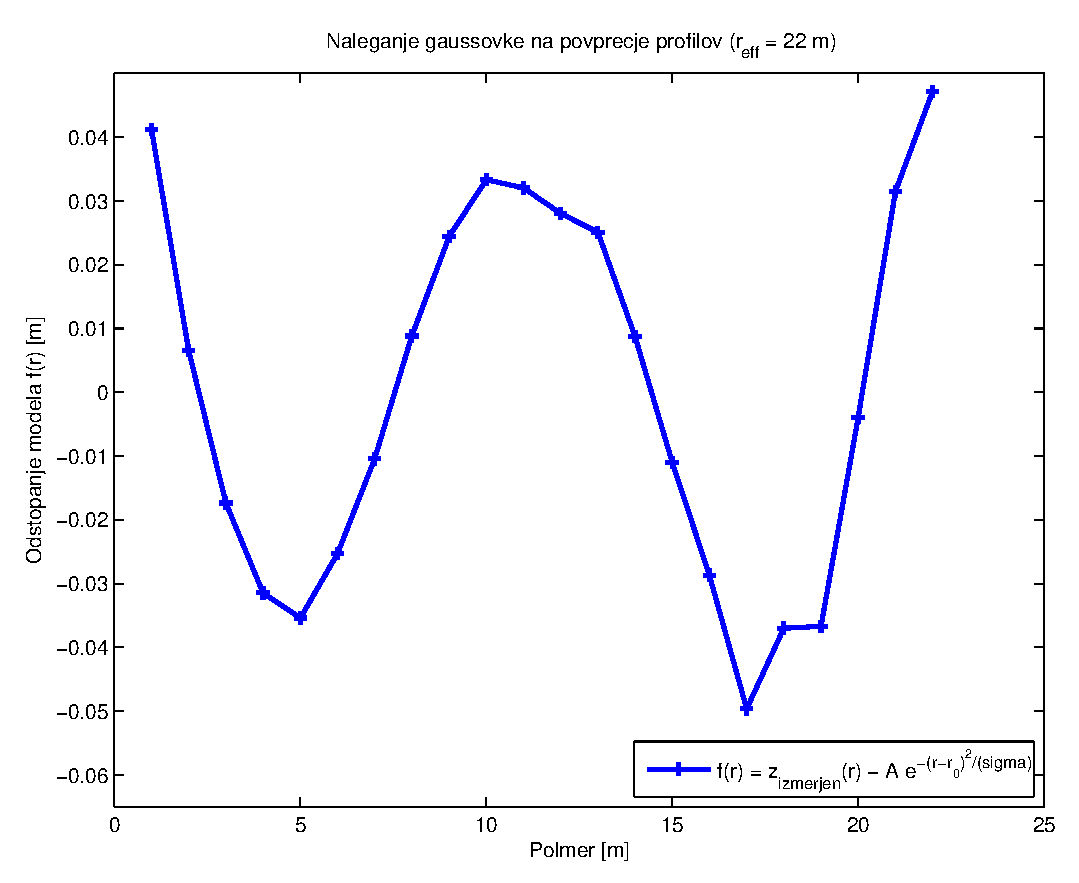
\includegraphics[width=10cm]{slike/menisija-profil-21-fit}
    \end{center}
    \caption{Povprečimo profile vrtač v velikostnem razredu $23,5m < r_{eff} < 24,5m$ po (\ref{povprecenje-profilov}), jim prilegamo Gaussovko (\ref{fit-vrtace}) in izrišemo ujemanje prileganja (\ref{ujemanje-fita}).}
    \label{fig:menisija-profil-21-fit}
  \end{figure}

Ker nam povprečna vrtača (Slika \ref{fig:menisija-vrtaca}) ne pove veliko, nadaljujemo tako, da Gaussovo funkcijo (\ref{fit-vrtace}) nalegamo na prej po enačbi (\ref{povprecenje-phi}) izračunanih profilih realnih vrtač in tako izluščimo parametre $\sigma$ in $A$ realnih vrtač.

Rezultata sta histograma na (Slika \ref{fig:menisija-globine-sigme-hist}).

  \begin{figure}[h!]
    \begin{center}
      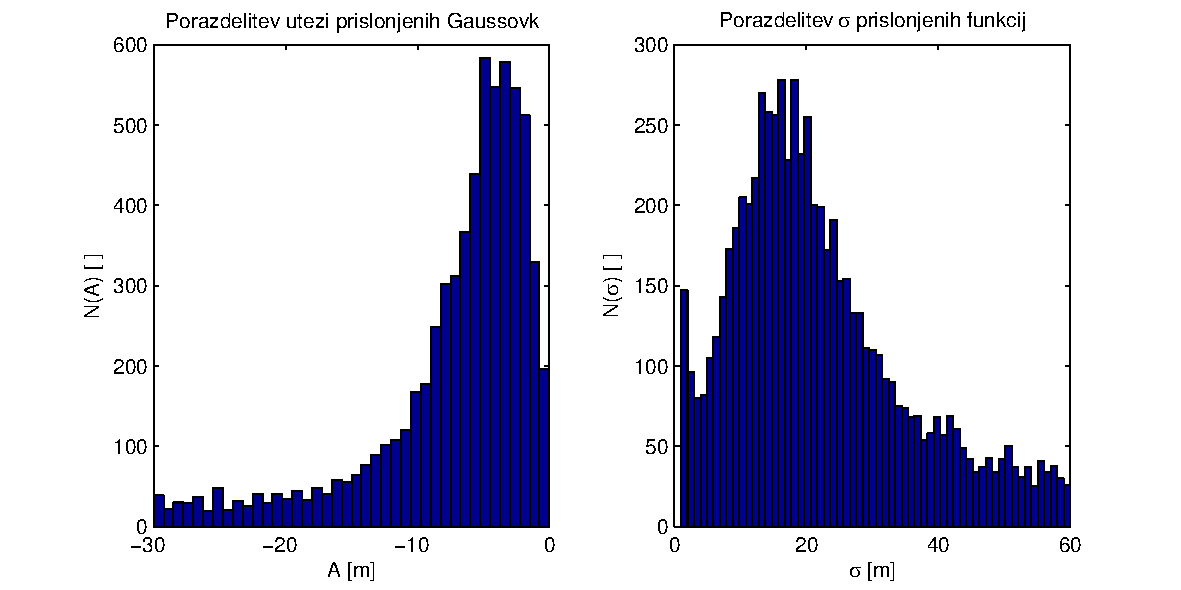
\includegraphics[width=13cm]{slike/menisija-visine-in-sigme-hist}
    \end{center}
    \caption{Vsem najdenim vrtačam prilegamo Gaussovo funkcijo (\ref{fit-vrtace}) in s tem izluščimo parametra A ter $\sigma$. Pridobljene podatke prikažemo na zgornjih histogramih. Izračunamo še povprečji ter standardni deviaciji količin $A$ in $\sigma$: $\bar A= -8,2m$, $\sigma_A=7,7m$, $\bar \sigma=24m$, $\sigma_{\sigma}=13m$.}
    \label{fig:menisija-globine-sigme-hist}
  \end{figure}

Iz vzorca izberemo vrtače tipičnih dimenzij ($5m < r_{eff} < 60m$). Izrišemo odvisnosti $\sigma (r_{eff})$, $A (r_{eff})$ ter $A(\sigma)$ in jim prilegamo linearne funkcije. Rezultat prikažemo na (Slika \ref{fig:menisija-sigma}).

  \begin{figure}[h!]
    \begin{center}
      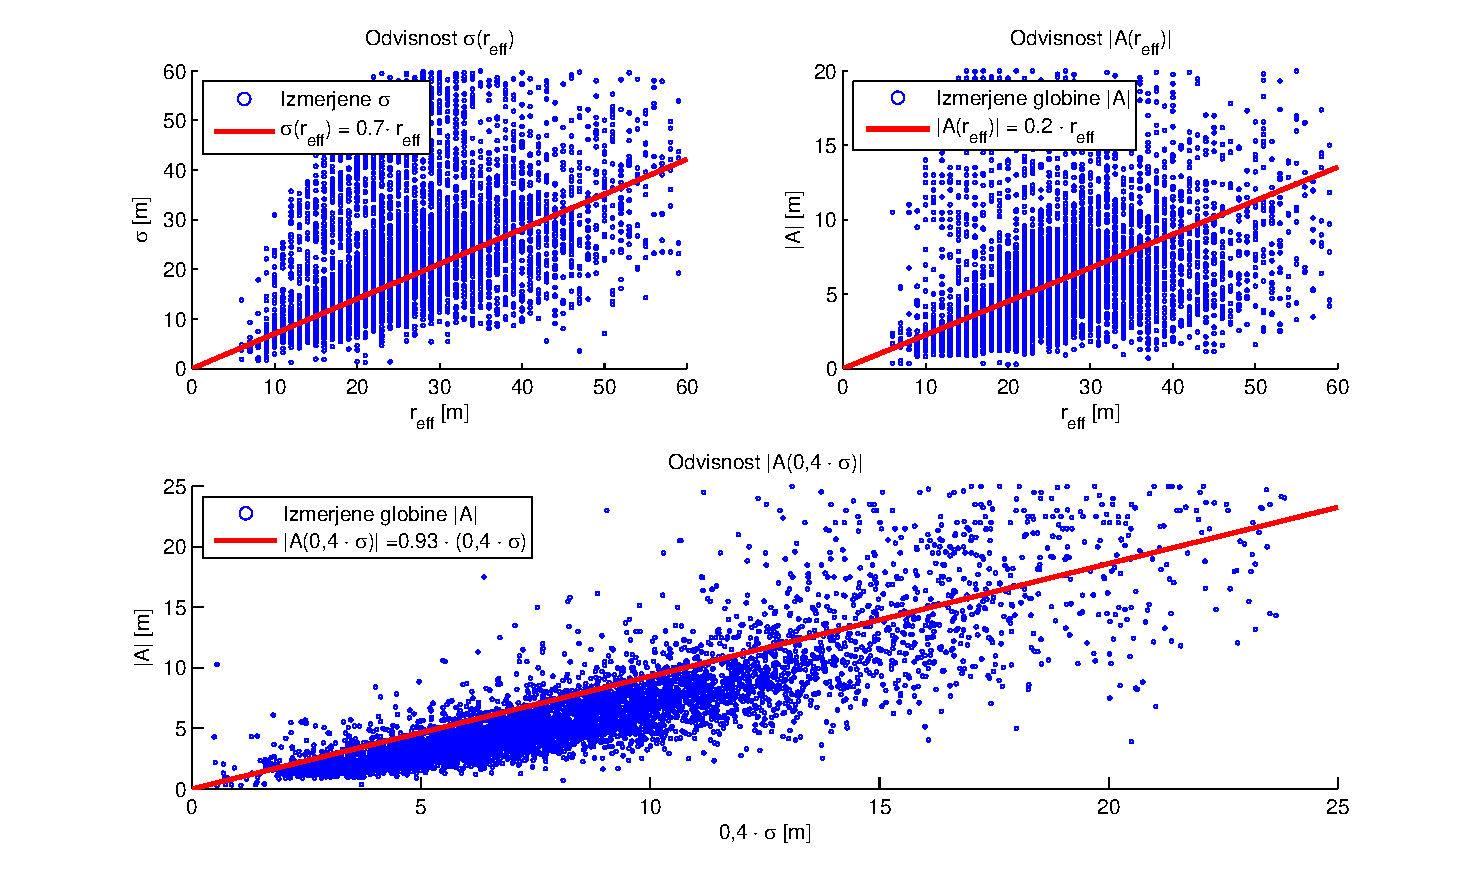
\includegraphics[width=14cm]{slike/menisija-A-sigma-reff}
    \end{center}
    \caption{Iz vzorca izberemo vrtače tipičnih dimenzij ($5m < r_{eff} < 60m$). Izrišemo odvisnosti $\sigma (r_{eff})$, $A (r_{eff})$ ter $A(\sigma)$ in jim prilegamo linearne funkcije. Vidimo, da izrisane odvisnosti niso naključne.}
    \label{fig:menisija-sigma}
  \end{figure}

  Na podlagi teh podatkov se zdi, da (\ref{fit-vrtace}) v grobem opiše profil idealne vrtače in ga bomo zato uporabili za analitično modeliranje.

  \chapter{Analitično modeliranje vrtač}
  \label{analiticno-modeliranje}

V tem poglavju bomo za opis časovne dinamike vrtač najprej podali definicije potrebne za opis rasti površin in denudacijo kraškega površja analogno modelirali kot stohastično rast oziroma usedanje površine. Nato bomo podali in komentirali več modelov rasti, ki se skladajo z uvodno tezo, da vrtače nastanejo na ravnem površju in rastejo dokler ne dosežejo stabilne oblike.

  \section{Usedanje površin}
  \label{definicije}

  V prvem poskusu opisa dinamike vrtač uporabimo definicije s področja rasti površin. Medtem ko pri rasti površin tipično študiramo stohastično priraščanje površin preko različnih mehanizmov, pri vrtačah predpostavimo, da kamnina na površju stohastično razpada in površina posledično upada. Na primeru balističnega usedanja uvedemo potrebne definicije. \cite{barabasi1995fractal}

Balistično usedanje preučuje model, kjer začnemo z ravnim površjem velikosti $L$. Na površje z razdalje večje od najvišje točke na površju in z naključne horizonalne pozicije $x$, padajo kvadratni delčki. Ti navpično padejo na povšje, ter se tam prilepijo. Tak proces pikazuje (Slika \ref{fig:bdep}).
Površje je meja med praznino in naloženimi delčki ter originalnim površjem.

    \begin{figure}[h]
      \begin{center}
        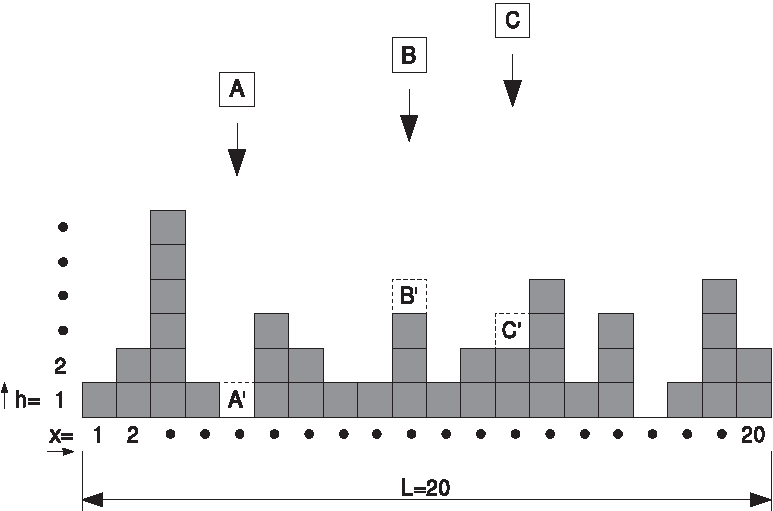
\includegraphics[width=8cm]{slike/bdep2.pdf}
      \end{center}
      \caption{Skica balističnega nalaganja v eni dimenziji. Delčki A, B in C ob različnih časih $t$ padejo poti površju in se prilepijo na lokacije A’, B’ in C’.}
      \label{fig:bdep}
    \end{figure}

Povprečno višino površja definiramo kot:

  \begin{equation}
    \langle h \rangle = \frac{1}{L} \sum_{i=1}^L h(i,t),
    \label{povprecna-visina}
  \end{equation}
kjer je $h(i,t)$ višina stolpca $i$ ob času $t$.

Če je usedanje delcev enakomerno porazdeljeno po $x$, je verjetnost, da se naslednji delec usede v točki $i$:
\begin{equation}
  p = \frac{1}{L},
\end{equation}
oziroma se bo z verjetnostjo
\begin{equation}
  q = 1 - p,
\end{equation}
usedel drugam.
Verjetnost, da bo poljuben stolpec po N padlih delcih dosegel višino $h$ je torej:
\begin{equation}
  P(h,N) = \binom{N}{h} p^h (1 - p)^{N - h}.
\end{equation}
Vepljemo čas kot $t = N / L$ in preračunamo:
\begin{align}
  \langle h \rangle &= \sum_{h=0}^{N} h P(h,N) \\
  &= \sum_{h=0}^{N} \binom{N}{h} h p^h q^{N - h} \\
  &= p \frac{\partial}{\partial p} \sum_{h=0}^{\infty} \binom{N}{h} p^h q^{N - h} \\
  &= p \frac{\partial}{\partial p} (p + q)^N \\
  &= p N (p + q)^{N-1} \\
  &= p N (p + 1 - p)^{N-1} \\
  &= N / L \\
  \langle h \rangle &= t.
\end{align}

Povprečna višina se bo torej povečevala linearno s časom:
\begin{equation}
  \langle h(t) \rangle \sim t.
\end{equation}

Hrapavost površja definiramo s standardno deviacijo višine površja od povprečne višine:
  \begin{equation}
    w(L,t) = \sqrt{\frac{1}{L} \sum_{i=1}^L (h(i,t)-\langle h(t) \rangle)^2}.
    \label{sirina-povrsine}
  \end{equation}

Poskusimo izraziti še $\langle h^2(t) \rangle $:
\begin{align}
  \langle h^2 \rangle &= \sum_{h=0}^{N} h^2 P(h,N) \\
  &= p \frac{\partial}{\partial p}p \frac{\partial}{\partial p} (p + q)^N \\
  &= p \frac{\partial}{\partial p} p N (p + q)^{N-1} \\
  &= p N (p + q)^{N-1} + p^2 N (N - 1) (p + q)^{N-2} \\
  &= p N (p + 1 - p)^{N-1} + p^2 N (N - 1) (p + 1 - p)^{N-2} \\
  &= p N + p^2 N^2 - p^2 N \\
  \langle h^2 \rangle &= t + t^2 - p \cdot t.
\end{align}

Hrapavost površja za balistično nalaganje je torej:
\begin{align}
  w(L,t) &= \sqrt{\langle (h - \langle h \rangle)^2\rangle} \\
  &= \sqrt{\langle h^2 \rangle - \langle h \rangle^2} \\
  &= \sqrt{t + t^2 - p \cdot t - t^2} \\
  &= \sqrt{(1-p)t} \\
  w(L,t) &\sim t^{1/2}.
\end{align}

Pri navadnem balističnem usedanju, kjer so višine stolpcev nekorelirane, se hrapavost površja s časom zgolj povečuje. Če pri verjetnosti za usedanje delca $p$ upoštevamo še na primer višino prvih sosednjih stolpcev, višina stolpcev sčasoma postane korelirana in hrapavost površja preneha rasti. \\
Sedaj si poglejmo celotno časovno odvisnost hrapavosti površja. Začnemo z ravno površino hrapavosti $w(L,t=0)=0$. Sledi kratko prehodno obdobje nekorelirane, Poissonove rasti, ko se delčki nekorelirano usedajo na ravno podlago. Kot smo ravnokar dokazali v tem obdobju velja:
\begin{equation}
  \begin{array}{lr} w(L,t) \sim t^{1/2} & \ t < t_b, \end{array}
\end{equation}
kjer je $t_b$ čas balističnega usedanja, ki je odvisen od mehanizma korelacije sosednjih stolpcev.
Zaradi korelacij med sosednjimi stolpci to obdobje ne traja dolgo, pač pa v času $t_b < t \ll t_s$ preide v obdobje rasti, kjer je $t_s$ čas zasičenja rasti hrapavosti. V obdobju rasti, predpostavimo da velja:
  \begin{equation}
    \begin{array}{lr} w(L,t) \sim t^\beta  & \ t_b < t \ll t_s, \end{array}
    \label{beta}
  \end{equation}
kjer je $\beta$ eksponent rasti, ki je odvisen od korelacijskega mehanizma in poda časovno dinamiko hrapavosti površja.

Po dolgem času rast površja preide v zasičeni režim, v katerem je površje popolnoma korelirano in se časovna rast hrapavosti ustavi ter sama hrapavost ni več odvisna od časa, doseže zasičeno vrednost $w_{sat}(L)$, ki je od velikosti sistema $L$ odvisna takole:

  \begin{equation}
    \begin{array}{lr} w(L,t_s) = w_{sat}(L) \sim L^\alpha & (t \gg t_s). \end{array}
    \label{alfa}
  \end{equation}

Eksponent hrapavosti $\alpha$ je tudi odvisen od korelacijskega mehanizma in nam pove kako je hrapavosti zasičenega površja odvisna od njegove velikosti. Če je $\alpha = 0$, je površje gladko, saj hrapavost površja s povečevanjem $L$ ne narašča. Za $\alpha > 0$ hrapavost površja divergira pri $L \rightarrow \infty$, tako površje je grobo. \cite{krim1993roughness}

Čas zasičenja $t_s$, ob katerem rast površja preide iz nenasičenega v nasičen režim, je odvisen od velikosti površja in je:
  \begin{equation}
    t_s \sim L^z,
    \label{z}
  \end{equation}
kjer je $z$ dinamični eksponent, ki je povezan z dinamiko hrapavosti površja.

Celotna dinamika hrapavosti pri balističnem naleganju je za različne velikosti površja prikazana na (Slika \ref{fig:barabasi}). Prvo koleno na grafu prikazuje prehod iz Poissonovega v režim rasti, ko se na sprva ravnem površju začne uveljavljati korelacija med stolpci. Obdobje rasti je tem daljše, čim večje je površje, katerega velikost podamo z $L$, čas pa je definiran kot $t=N/L$. Po obdobju rasti so stolpci popolnoma korelirani, površje še vedno prirašča, njegova hrapavost pa ostaja konstantna.

    \begin{figure}[h]
      \begin{center}
        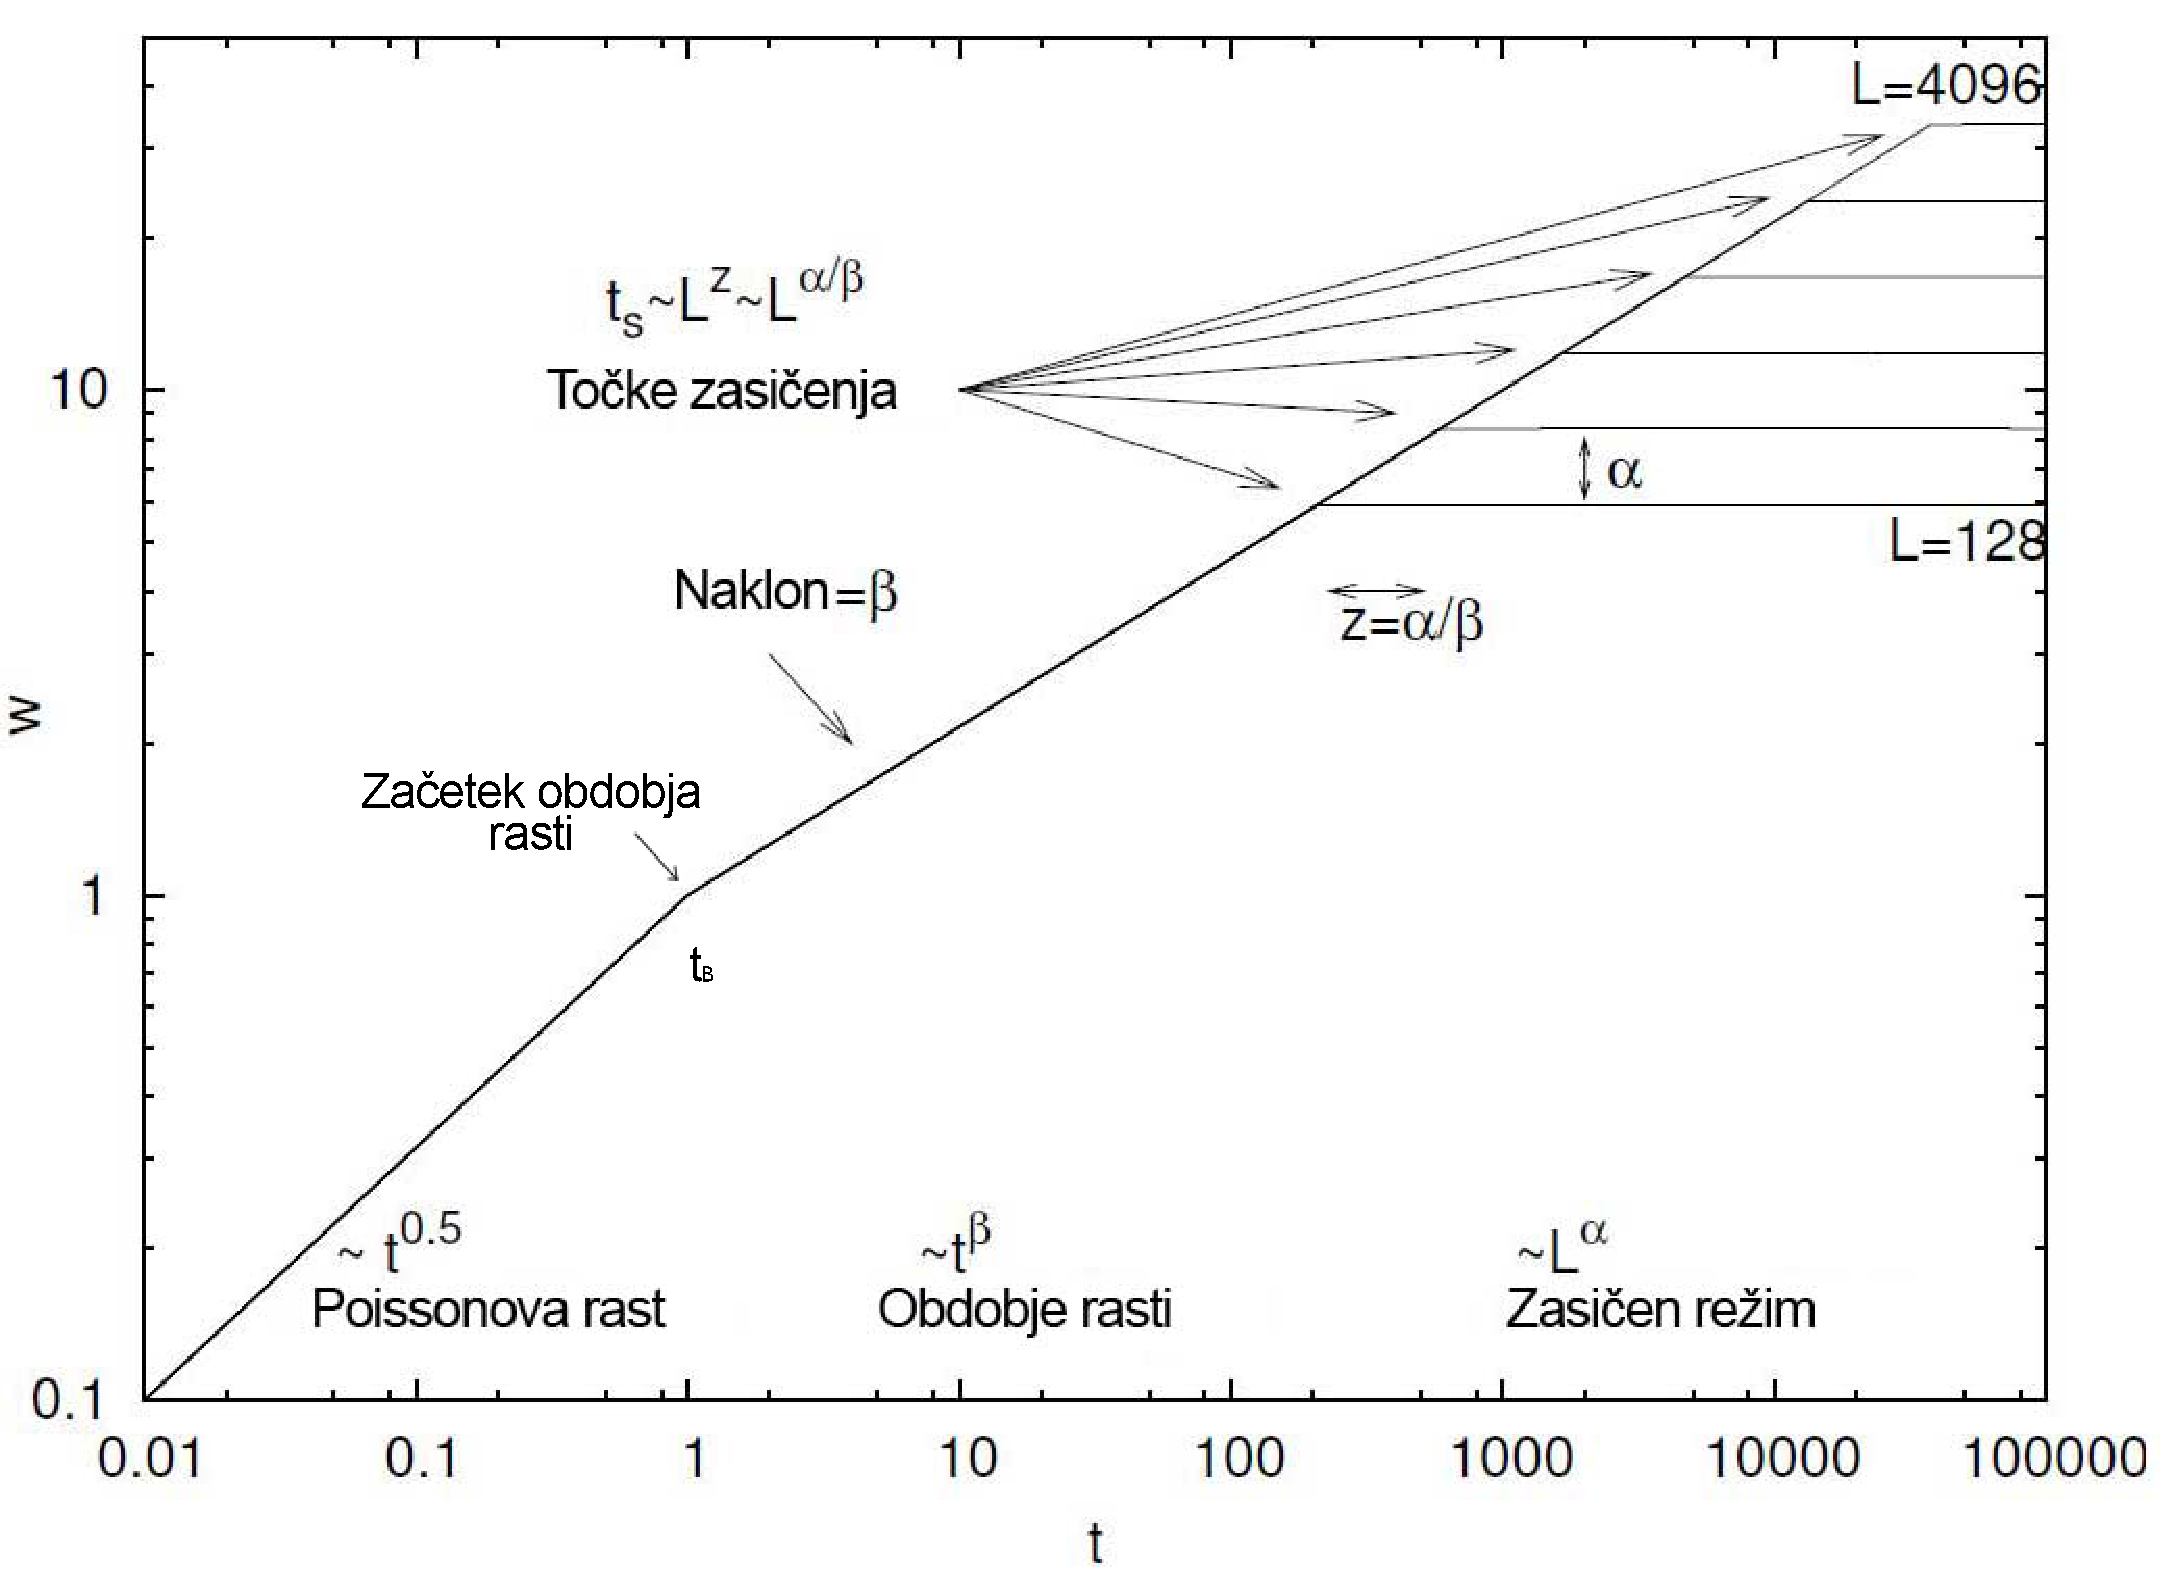
\includegraphics[width=10cm]{slike/bdep3.pdf}
      \end{center}
      \caption{Idealni potek hrapavosti površja pri balističnem naleganju, za različne velikosti sistema L. Začnemo z ravnim površjem ($w(L,t)=0$) in po kratkem prehodnem obdobju Poissonove rasti ($w(L,t) \sim t^{1/2}$), preidemo v obdobje rasti ($w(L,t) \sim t^{\beta}$). To se zaključi po času $t_s \sim L^z$ in preidemo v zasičen režim ($w(L,t) = w_{sat}(L) \sim L^{\alpha}$). Vir \cite{schwettmann2003}.}
      \label{fig:barabasi}
    \end{figure}

Eksponenti $\alpha$, $\beta$ in $z$ med seboj niso neodvisni, pač pa med njimi lahko izpeljemo določene relacije lestvičenja podobno kot pri kritičnih eksponentih v teoriji faznih prehodov drugega reda.\cite{stanley1987introduction}. Poskusimo izpeljati te povezave.

Iz (Slika \ref{fig:barabasi}) in zveze (\ref{alfa}) vidimo, da se krivulje $w(L,t)/w_{sat}(L)$ zasičijo pri isti konstantni vrednosti, ne glede na velikost sistema $L$. Iz zveze (\ref{z}) pa vidimo, da se bodo hrapavosti površij zasitile po istem karakterističnem času $t/t_s$. Sklepamo, da je $w(L,t)/w_{sat}(L)$ funkcija $t/t_s$, torej:

  \begin{equation}
    \frac{w(L,t)}{w_{sat}(L)} \sim f(\frac{t}{t_x}),
  \end{equation}
kjer je $f(t/t_s)$ funkcija lestvičenja. Vstavimo $w_{sat}$ in $t_s$, po zvezah (\ref{alfa}), (\ref{z}) in dobimo Family-Vicsek relacijo lestvičenja:

  \begin{equation}
    w(L,t) \sim L^\alpha f(\frac{t}{L^z}).
    \label{family-vicsek}
  \end{equation}

Za $f(u)$ velja:
  \begin{equation}
    f(u) \propto \left \{ \begin{array}{lr} u^{\beta} & \ u\ll 1 \\
      1 & \ u\gg1\end{array}, \right.
    \end{equation}
kjer je $\beta$ eksponent rasti in $u=\frac{t}{t_s}$.

Sedaj si ogledamo (Slika \ref{fig:barabasi}). Če se točki zasičenja $(t_s,w(t_s))$ približamo z leve, vidimo, da po (\ref{beta}) velja $w(t_s) \sim t_s^\beta$. Hkrati pa, da če se isti točki približamo z desne po (\ref{alfa}) velja $w(t_s) \sim L^\alpha$. Torej $t_s^\beta \sim L^\alpha$ in po (\ref{z}) sledi zakon o lestvičenju:

    \begin{equation}
      z = \frac{\alpha}{\beta}.
    \end{equation}

To je torej zveza med eksponenti lestvičenja, ki jo lahko izpeljmo.

Uvedli smo potrebne definicije za opis stohastičnega usedanja površin, ki ga bomo sedaj uporabili za opis denudacije kraškega površja. Proces denudacije, ki oblikuje kraške vrtače je seveda drugačen od balističnega usedanja, ki smo ga uporabili za predstavitev definicij. Najpomembnejša razlika je, da je model rasti površin inverzen modelu denudacije in si ga zamišljamo kot negativno rast površja. Seveda pričakujemo, tudi korelacijo med sosednjimi točkami površja.

Sedaj predlagamo model stohastičnega usedanja in izračunamo hrapavost v njegovem zasičenem režimu, ter jo primerjamo z izmerjeno hrapavostjo na pravem kraškem površju z vrtačami.

\section{Merjenje hrapavosti Menišije}
\label{hrapavost}

V uvodu smo postavili tezo, da so vse vrtače stare, stabilne oblike. Ko jih opišemo z definicijami rasti površin, domnevamo da so starejše od časa zasičenja ($t_s$) in zanje velja zveza (\ref{alfa}). Predelamo jo v $ w_{sat}=C \cdot L^\alpha $ in dobimo sledečo zvezo za eksponent hrapavosti starega površja:
    \begin{equation}
      \alpha = \frac{\partial ( ln (w_{sat}) ) }{\partial ( ln L )}.
      \label{alpha-numeric}
    \end{equation}

Ta eksponent skušamo sedaj oceniti iz dobljenih eksperimentalnih podatkov.

Iz LiDARskega modela Menišije izrezujemo plakete velikosti $L\times L$ in na višinskih točkah, ki jih vsebujejo izračunamo standardno deviacijo, oziroma hrapavost ${w}_{sat}$. Odvisnost $ln(w_{sat}(ln(L^2)))$ izrišemo na (Slika \ref{fig:menisija-alfa}) in z grafa odberemo rezultat:
\begin{equation}
  \bar w(ln(L^2)) = \alpha \cdot ln(L^2) + c = 0,71 \cdot  ln(L^2) - 1,86,
\end{equation}
torej:
\begin{equation}
  \alpha =  0,71 \pm 0.01.
\end{equation}
\begin{figure}[h!]
  \begin{center}
    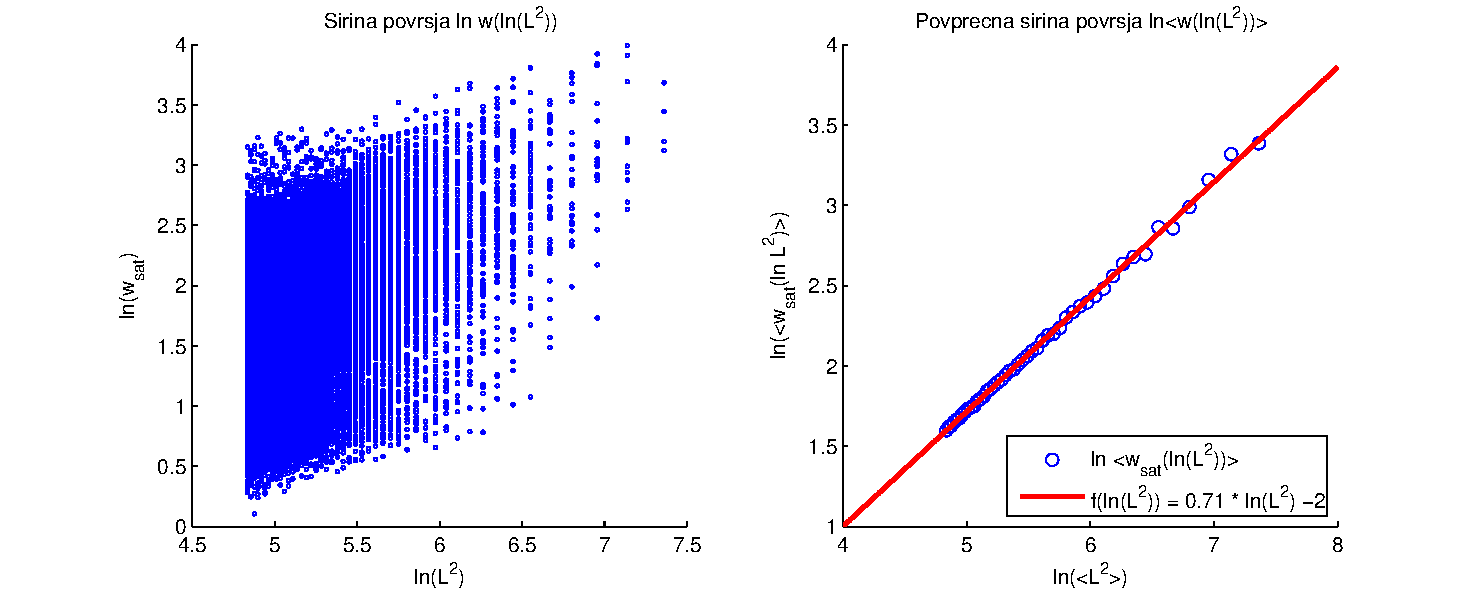
\includegraphics[width=14.5cm]{slike/menisija-alfa-3d.pdf}
  \end{center}
  \caption{Izračunane hrapavosti $ln({w}_{sat}(L^2))$ izrišemo na levi sliki. Na desni pa za vsak $ln(L^2)$ izračunamo povprečno hrapavost $ln(\bar w_{sat}(ln(L^2)))$ in nato prilegamo premico. Točke na $x$ osi se zaradi diskretnih velikosti plaket $L\times\L$ pojavijo v diskretnih korakih.}
  \label{fig:menisija-alfa}
\end{figure}

Izmerili smo hrapavost površja Menišije. Sedaj skušamo osmisliti dobljene fenomenološke rezultate z formalnim (matematičnim) modelom, ki bo v zasičenem režimu dal podobno hrapavost. Tu se opremo na stohastični model rasti površin, ki so ga postavili Kardar, Parisi in Zhang \cite{kardar1986dynamic}.

    \section{Model Kardar-Parisi-Zhang}

    Za modeliranje nastanka vrtač najprej privzamemo, da ima proces poleg stalne hitrosti denudacije kamnine $v$ še stohastično komponento $\eta(\mathbf{x},t)$:
\begin{equation}
  \frac{\mathrm{d} h}{\mathrm{d} t} \bigg|_{denudacija} = v + \eta(\mathbf{x},t),
\end{equation}
kjer $\mathbf{x}$ predstavlja lokacijo na površini ravnine, $v$ povprečno hitrost denudacije, $h(\mathbf{x},t)$ pa višino površine v tej točki ob času $t$. 

Za $\eta (\mathbf{x},t)$ privzamemo, da je časovno in prostorsko nekoreliran Gaussov šum: 
\begin{equation} 
  \langle \eta(\mathbf{x},t) \rangle=0,
\end{equation}
in:
\begin{equation}
  \langle \eta(\mathbf{x},t) \eta(\mathbf{x'},t')\rangle = 2 D \delta^d(\mathbf{x}-\mathbf{x'})(t-t'),
\end{equation}
kjer je $D$ parameter modela in $d$ število dimenzij prostora.

Taka površina raste kot:
\begin{equation}
  h(\mathbf{x},t) = v \cdot t + \int_0^t \mathrm{d} t' \eta (\mathbf{x},t).
\end{equation}

Zaradi časovne nekoreliranosti šuma $\eta({\mathbf{x},t})$ bi tako površje ohranjalo začetno obliko:

\begin{equation}
  \langle h(\mathbf{x},t) \rangle = v \cdot t + \int dt \langle \eta \rangle = v \cdot t.
\end{equation}

Ker je razpadanje kamnine počasen proces in se iz podlage odkrušeni kamni lahko premikajo, privzamemo v naš model še difuzijski člen:
\begin{equation}
  \frac{\mathrm{d} h}{\mathrm{d} t} \bigg|_{difuzija} = D \nabla^2 h,
\end{equation}
kjer je $D$ utež 'površinske napetosti', ki opisuje površinsko difuzijo. Ta člen očitno deluje 'entropijsko'  saj želi izravnavati stohastične variacije površine. Njegova vloga je podobna kot jo ima Fickov zakon pri difuziji delcev v raztopinah.

\begin{comment}
[TODO]Difuzija je 'entropijska' in kaže vedno invarianti gradienta. Sledi kratek opis difuzije v tekočini.[TODO]
\end{comment}

Končno privzamemo še, da je smer mikroskopske denudacije kamnine obrnjena v kamnino, v smeri normale površja (Slika \ref{fig:KPZ}). 
\begin{figure}[h!]
  \begin{center}
    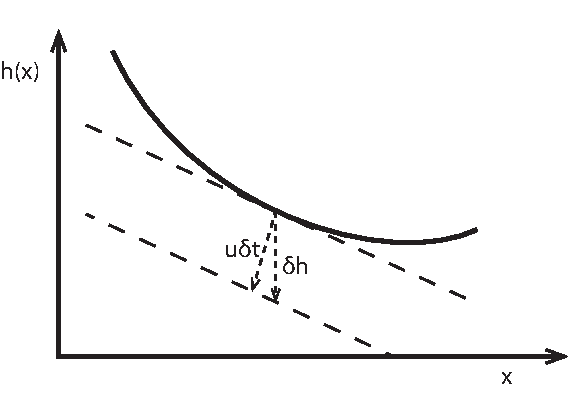
\includegraphics[width=6cm]{slike/denudacija}
  \end{center}
  \caption{Denudacijo privzamemo v smeri normale površja. $u$ je hitrost mikroskopske denudacije v smeri normale.}
  \label{fig:KPZ}
\end{figure}

Zapišemo Pitagorov izrek za $\delta h$:
\begin{equation}
  \delta h = \sqrt{(u \delta t)^2 + (u \delta t \nabla h)^2} = u \delta t \sqrt{1 + (\nabla h)^2},
  \label{kpz-normala}
\end{equation}
kjer je $u$ hitrost mikroskopske denudacije kamnine v smeri normale površja (Slika \ref{fig:KPZ}). Privzamemo $|\nabla h| \ll 1$ in razvijemo (\ref{kpz-normala}) v:
\begin{equation}
  \frac{\partial h}{\partial t} \bigg|_{nelinearno} \simeq u + \frac{u}{2} (\nabla h)^2 + \dots.
\end{equation}

Zanemarimo višje člene in zapišemo:
\begin{equation}
  \frac{\partial h}{\partial t} \bigg|_{nelinearno} = u + \frac{u}{2} (\nabla h)^2
\end{equation}

\begin{comment}
    \begin{figure}[h]
      \begin{center}
        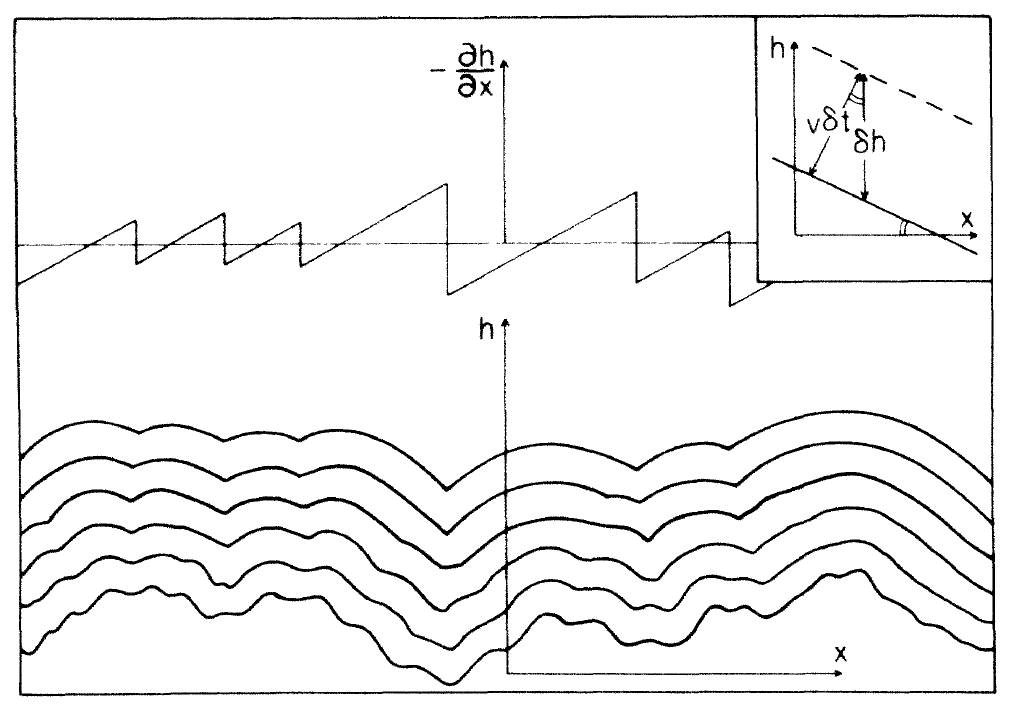
\includegraphics[width=9cm]{slike/kpz.png}
      \end{center}
      \caption{Zaporedni profili deterministične rasti, priraščanje v smeri normale površja je prikazano desno zgoraj.}
      \label{fig:kpz}
    \end{figure}
\end{comment}

Pripravljene člene zdužimo v enačbo:
\begin{equation}
  \frac{\partial h}{\partial t} = \frac{\partial h}{\partial t} \bigg|_{denudacija} + \frac{\partial h}{\partial t} \bigg|_{difuzija} + \frac{\partial h}{\partial t} \bigg|_{nelinearno},
  \label{KPZ1}
\end{equation}
oziroma:
\begin{equation}
  \frac{\partial h}{\partial t} = v + D \nabla^2 h + u + \frac{u}{2} (\nabla h)^2 + \eta (\mathbf{x},t).
  \label{KPZ2}
\end{equation}

Postavimo se v premikajoč koordinatni sistem, ki se premika s hitrostjo $v + u$ v smeri osi $h$ in dobimo Kardar-Parisi-Zhang enačbo (\cite{kardar1986dynamic}):
\begin{equation}
  \frac{\partial h}{\partial t} = D \nabla^2 h + \frac{u}{2} (\nabla h)^2 + \eta (\mathbf{x},t).
  \label{KPZ}
\end{equation}

Če vzamemo nastavek:
\begin{equation}
  h(\mathbf{x},t) = \frac{2 D}{u} log(Z(\mathbf{x},t)),
\end{equation}
dobimo difuzijsko enačbo v časovno odvisnem naključnem potencialu:
\begin{equation}
  \frac{\partial Z}{\partial t} = D \nabla^2 Z + \frac{u}{2 D} \eta(\mathbf{x},t) Z,
  \label{KPZ3}
\end{equation}

Primerjajmo to z običajno difuzijsko enačbo za gostoto ob prisotnosti izvirov:
\begin{equation}
  \frac{ \partial \rho}{ \partial t} = \mathbf{\nabla} \cdot \mathbf{j} = \mathbf{\nabla} (D \cdot \mathbf{\nabla} \rho) + \mathbf{\nabla} \cdot \mathbf{j_0},
  \label{dinamicna-splosna-3}
\end{equation}
kjer je zadnji člen na desni gostota izvirov, predzadnji pa je Fickov člen. Če za jakost izvirov velja:
\begin{equation}
  \mathbf{\nabla} \cdot \mathbf{j_0} = \frac{\partial \rho}{\partial t}\bigg|_{0} = C \cdot \rho.
  \label{jakost-izvirov}
\end{equation}

Potem vidimo, da (\ref{KPZ3}) ustreza izvorom s stohastično jakostjo $C$, ki je odvisna še od $C=C(\mathbf{x},t)$. Tu imamo torej že neke vrste stohastičen reakcijsko difuzijski sistem pri katerem pa je stohastičen del linearno odvisen od gostote. Kasneje bomo ugotovili, da bi lahko to tudi posplošili na nelinearne primere.

Formalno se da rešitev (\ref{KPZ3}) dobiti v obliki:
\begin{equation}
  h(\mathbf{x},t) = \frac{2 D}{\lambda} ln \left( \int_{-\infty}^{\infty} \frac{d^d \xi}{(4 \pi D t)^{d/2}} \cdot exp \left[-\frac{(x-\xi)^2}{4 D t} + \frac{u}{2 D}h(\xi,0) \right] \right),
\end{equation}
kjer je $d$ število dimenzij v prostoru.

    To formalno rešitev avtorji \cite{kardar1986dynamic} nato v Fourierovem prostoru s pogojem za beli šum perturbativno rešijo (\ref{KPZ}). Tej izpeljavi tukaj ne bomo sledili, ker je formalno prezahtevna. Zato se bomo poglobili le v numerično reševanje KPZ enačbe. Končno pokažejo, da za stohastično priraščanje površja velja: $z = \frac{3}{2}$ in $\alpha=\frac{1}{2}$. Rezultat se relativno dobro ujema z $\alpha =  0,71 \pm 0.01$ namerjenim v (Poglavje \ref{hrapavost}).

Da bi kvalitativno ocenili kakšno površje nastane z stohastično denudacijo površja, napravimo preprosto numerično simulacijo. Začnemo z ravnim površjem velikosti $80\times80$ točk, določimo časovni korak $\mathrm{d}t=10^{-3}$ in $10^6$-krat izračunamo:
\begin{equation} 
  h_{i+1} = h_i - dt (D \nabla^2 h_i + \frac{u}{2} (\nabla h_i)^2 + \eta (\mathbf{x},t)),
\end{equation}
kjer je $h_{i+1}$ nova vrednost v obravnavani točki, $h_{i}$ stara vrednost v obravnavani točki, $\eta (\mathbf{x},t) \in [0,1]$ in določimo $D = u = 1$. (Slika \ref{fig:KPZ-numericno}) je primer tako simuliranega površja.

Končno stanje površja pri tem ni statično, med koraki prihaja do manjših premikov. Vendar pa so oblike, ki na površju nastanejo, stabilne ter med seboj podobne po obliki in velikosti.

    \begin{figure}[h]
      \begin{center}
        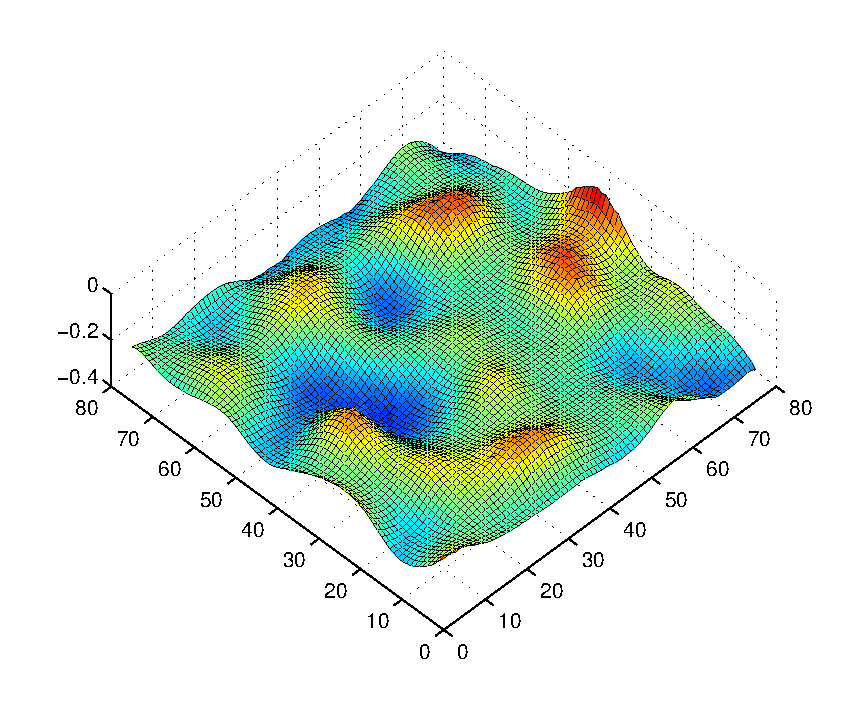
\includegraphics[width=10cm]{slike/KPZ-numericno}
      \end{center}
      \caption{Numerična simulacija po Kardar-Parisi-Zhang enačbi razvijajočega se površja po $10^5$ korakih.}
      \label{fig:KPZ-numericno}
    \end{figure}

Na površju na (Slika \ref{fig:KPZ-numericno}) opazimo, da so se na sprva ravnem površju razvile globeli, med seboj podobnih si oblik in globin. Originalne ravnine, s katero smo simulacijo začeli ne prepoznamo več. Po prvi oceni se zdijo globeli podobne vrtačam, a bi za resno primerjavo morali simulirati precej večje področje, kar je računsko zahtevna naloga. Tako površje bi nato obdelati z enakimi orodji, kot smo jih uporabili na digitalnem modelu Menišije, da bi izločili posamezne globeli in nato izračunali porazdelitve $N(A)$, $N(\sigma)$ in $A(\sigma)$, ki bi nam hitro pokazale, če model ne bi bil ustrezen.

Zanimiv eksperiment bi bil tudi, da bi vzeli digitalni model Menišije in na njem izvedli $10^5$ korakov Kardar-Parisi-Zhang dinamike, ter nato primerjali porazdelitve $N(A)$, $N(\sigma)$ in $A(\sigma)$ z originalnimi. Tako bi pokazali, da je oblika Menišije stabilna in da jo vzdržuje podobna ali enaka stohastična dinamika, kot smo jo predlagali.


\section{Reakcijsko-difuzijski model dinamike vrtač}

Do sedaj smo modelirali vrtače kot posledico stohastičnega procesa. Kardar-Parisi-Zhang je neke vrste stohastična reakcijsko difuzijska enačba, kot smo pokazali v prejšnjem podpoglavju. Zdi se, da Kardar-Parisi-Zhang model nakazuje, da obstaja povezava med reakcijsko difuzijskimi modeli in dinamiko vrtače. Zato poskusimo modelirati rast vrtač še z nekaj drugimi reakcijsko difuzijskimi modeli. Ker nimamo jasnega modela na katerega bi se oprli je ta problem bolj kompleksen, saj mora v upoštevati vse dejavnike rasti ene same vrtače. 

Ker mikroskopskega modela take dinamike ne moremo postaviti, si ogledamo nekaj fenomenoloških modelov rasti, ki temeljijo na reakcijsko-difuzijski dinamiki (\ref{dinamicna-splosna}) opisa rasti, ki jo potrjuje tudi Kardar-Parisi-Zhang model. Predlagani modeli so primerni za opis prostorsko porazdeljenih kemijskih reakcij in mehanskega transporta materiala v vrtačah. Ti modeli predpostavijo, kako na neko količino vpliva izbrana deterministična dinamika in difuzija.

Predlagali bomo torej več modelov, kako naj globina in oblika vrtače vpliva na njeno poglabljanje. Opirali se bomo na geomorfološko tezo, da globlja in večja kot je vrtača, več vode zbira in se posledično hitreje poglablja. Hkrati pa ima tudi nekakšen zaviralni mehanizem, ki rast v določenem trenutku zaustavi, saj bi sicer dobili brezno.
Zapišimo Kardar-Parisi-Zhang enačbo v obliki:
\begin{equation}
  \frac{ \partial h(t,x) }{ \partial t} = D \nabla^2 h + F(h),
  \label{dinamicna-splosna}
\end{equation}
kjer je $F(h)$ linearna funkcija $h$ s stohastično jakostjo kot je razvidno iz (\ref{KPZ3}). Sedaj predpostavimo obratno, namreč, da je jakost izvorov sicer deterministična funkcija $h$, ampak ni več linearna funkcija kot pri Kardar-Parisi-Zhangovi enačbi. Ob odsotnosti boljših morfoloških modelov nastanka vrtač se zdi to smiselna posplošitev.

Najprej ločeno pogledamo različne variacije determinističnega člena $F(h)$ za (\ref{dinamicna-splosna}). Izbor determinističnih členov rasti $F(h)$ je delno povzet po \cite{kandler2010population}. Medtem ko je pri Kardar-Parisi-Zhang modelu $F(h)$ stohastičen člen, sedaj torej raje predpostavimo, da je rast v primeru posamezne vrtače deterministična in v splošnem nelinearna.

\begin{comment}
    \begin{equation}
      F(h) = \left \{ \begin{array}{lr} 
        a \cdot h \\
        a \cdot h \cdot (1 - \frac{h}{K}) \\
        a \cdot (K - h) \\
        - h \cdot e^{-a t}
      \end{array}. \right. 
      \label{dinamicna-variacije}
    \end{equation}
\end{comment}

\subsection{Eksponentna rast}

Prvi deterministični nastavek za rast nam da dinamiko eksponentne rasti, ki jo izpeljemo tako da postavimo, da je hitrost naraščanja količine $h(t)$ sorazmerna z vrednostjo te količine. Dobimo enačbo:
    \begin{equation}
      \frac{\partial h(t)}{\partial t} = a \cdot h(t),
      \label{dinamicna-eksponentna}
    \end{equation}
ki jo reši funkcija:
    \begin{equation}
      h(t) = h_0 e^{a t}.
      \label{dinamicna-eksponentna-resitev}
    \end{equation}

Pri variaciji koeficienta rasti $a$ narišemo več rešitev:

    \begin{figure}[h]
      \begin{center}
        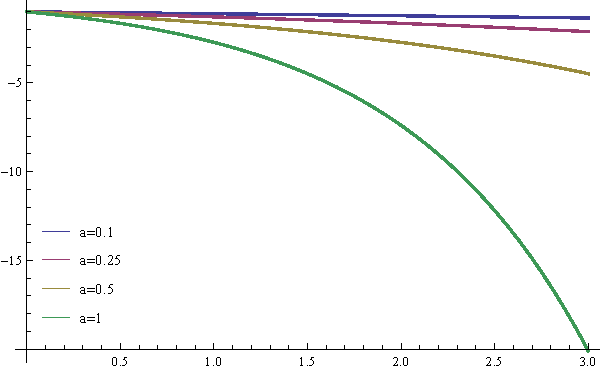
\includegraphics[width=7cm]{slike/eksponentna-rast}
      \end{center}
      \caption{Vzeli smo začetno vrednost $h_0 = -1$ in variirali vrednost $a$. \newline $a=0,1;0,25;0,5;1$.}
      \label{fig:eksponentna-rast}
    \end{figure}

Če velja $a > 0$, bomo vedno dobili neomejeno eksponentno rast, ki je v omejenih intervalih uporaben model za npr. opis rasti populacij držav, širjenje virusov, jedrskih verižnih reakcij, itn. Uporabnost modela se konča, ko se sistem zasiti - to je, ko zmanjka virov, ki rast poganjajo (če gledamo dane primere - ko zmanjka hrane, celic, jeder).\\
Pri vrtačah pričakujemo, da bo njihova rast na nek način odvisna od njihove globine, saj se voda steka proti nižjim točkam in tam povzroča hitrejšo denudacijo. Eksponentno rast bi torej pričakovali, če bi v naravi obstajale tudi zelo globoke vrtače, a takšnih eksperimentalno ne opazimo. Sklepamo torej, da je eksponentna rast v vrtačah v nekem obdobju razvoja možna, a pri starih, ravnovesnih vrtačah prevlada drugačna dinamika.


\subsection{Omejena eksponentna rast}

Model omejene eksponentne rasti predpostavi, da je hitrost rasti količine $h(t)$ tem večja, čim dlje je od nosilne kapacitete sistema $K$. To zapišemo v enačbo:
    \begin{equation}
      \frac{\partial h(t)}{\partial t} = a \cdot ( K - h(t) ) = a K - a h(t),
      \label{dinamicna-omejena-eksponentna}
    \end{equation}
in jo rešimo z:
   \begin{equation}
      h(t) = K - (K - h_0) e^{-a t}.
      \label{dinamicna-omejena-eksponentna-resitev}
    \end{equation}

Rezultat izrišemo na (Slika \ref{fig:omejena-eksponentna-rast}) ob variiranju začetne vrednosti $h_0$ ter koeficienta rasti $a$.

    \begin{figure}[h]
      \begin{center}
        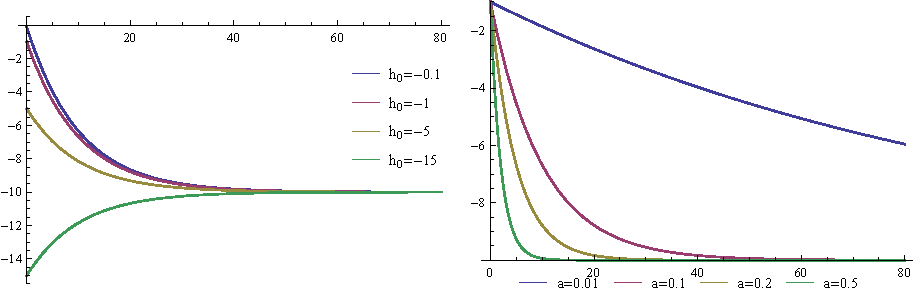
\includegraphics[width=14cm]{slike/omejena-eksponentna-rast}
      \end{center}
      \caption{Omejena eksponentna rast po (\ref{dinamicna-omejena-eksponentna-resitev}). Vzeli smo $K=-10$ in variirali ostale parametre. V prvem primeru smo pri $a=0,1$ vzeli $h_0=-0,1;-1;-5;-15$. V drugem pa pri $h_0=-1$, $a=0.01;0.1;0.2;0,5$.}
      \label{fig:omejena-eksponentna-rast}
    \end{figure}

    Medtem ko je omejena eksponentna rast podobna logistični, po tem, da se ustali pri $K$, pa ima logistična v začetku položnejšo rast. Omejena eksponentna rast se uporablja za modeliranje sistemov, v katerih dinamiko poganjajo zunanji dejavniki, medtem ko znotraj sistemov ni interakcij, na primer pri širjenju informacij v družbi preko medijev.\\
V začetku hitra rast, ki se na koncu ustali bi bila lahko primeren model za vrtače in se zdi primernejša od čisto eksponentne rasti.


\subsection{Logistična rast}

V modelu logistične rasti postavimo, da je hitrost spreminjanja količine $h(t)$ sorazmerna z vrednostjo te količine in razdaljo ($1 - \frac{h(t)}{K}$) do neke fizikalne omejitve sistema (npr. količine hrane v okolju, življenjskega prostora, itn). $K$ imenujemo nosilna kapaciteta sistema, $a$ pa koeficient rasti. To zapišemo v enačbo:
    \begin{equation}
      \frac{\partial h(t)}{\partial t} = a \cdot \left( 1 - \frac{h(t)}{K} \right) h(t),
      \label{dinamicna-logisticna}
    \end{equation}
ki jo reši funkcija:
    \begin{equation}
      h(t) = \frac{h_0 K e^{a t}}{K + h_0 (e^{a t}-1)}.
      \label{dinamicna-logisticna-resitev}
    \end{equation}

Rezultat prikažemo z variiranjem parametrov $h_0$ in $a$ na (Slika \ref{fig:logisticna-rast}).
    \begin{figure}[h]
      \begin{center}
        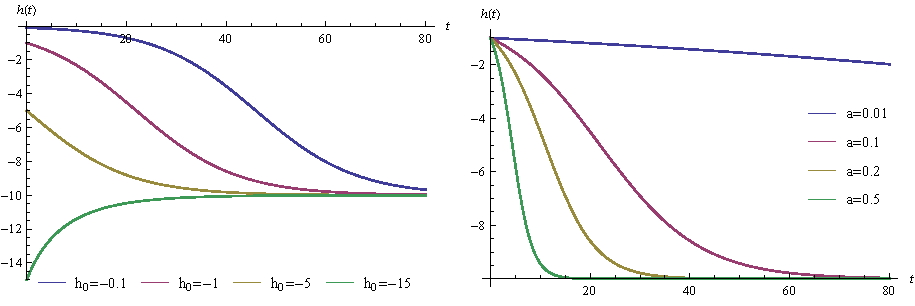
\includegraphics[width=14cm]{slike/logisticna-rast}
      \end{center}
      \caption{Logistična rast po (\ref{dinamicna-logisticna-resitev}). Vzeli smo $K=-10$ in variirali ostale parametre. V prvem primeru smo pri $a=0,1$ vzeli $h_0=-0,1;-1;-5;-15$. V drugem pa pri $h_0=-1$, $a=0.01;0.1;0.2;0,5$.}
      \label{fig:logisticna-rast}
    \end{figure}

    Vidimo, da ne glede na izbiro začetne točke $h_0$, vrednost h(t) konvergira proti vrednosti $K$. Torej je rast omejena s kapaciteto sistema K.
    Če funkcijo (\ref{dinamicna-logisticna-resitev}) Taylorjevo razvijemo, vidimo, da je rast, kjer $h(t) \ll K$, približno $a h(t)$. V območju, kjer je $h(t)$ bližji $K$, pa postane drugi člen v razvoju $-a h(t)^2 / K$ pomembnejši in rast se po dolgem času ustavi.\\
    Model logistične rasti se uporablja za modeliranje človeških in živalskih populacij, rasti tumorjev, širjenje inovacij v družbi in sprememb v jeziku. Zaradi na začetku in koncu počasne rasti pa se zdi zanimiv kandidat za modeliranje dinamike vrtač.


    \subsection{Gompertzova rast}

    Model Gompertzove rasti dopolni eksponentno rast tako, da koeficient rasti $a$ iz enačbe za eksponentno rast (\ref{dinamicna-eksponentna}) s časom spreminja po predpisu:
    \begin{equation}
      a(t) = a_0 \cdot e^{- k t},
      \label{dinamicna-gompertzova-faktor}
    \end{equation}
kjer je $k > 0$ koeficient pojemanja rasti, $a_0$ pa začetni koeficient rasti.
To nam da enačbo:
    \begin{equation}
      \frac{\partial h(t)}{\partial t} = a(t) \cdot h(t) = a_0 e^{ -k t} h(t),
      \label{dinamicna-gompertzova}
    \end{equation}
in rešitev:
    \begin{equation}
      h(t) = h_0 \cdot e^{\frac{a_0}{k}(1-e^{-kt})}.
      \label{dinamicna-gompertzova-resitev}
    \end{equation}

V časovni limiti pa tudi asimptotsko rešitev:
    \begin{equation}
      h(t) = h_0 \cdot e^{\frac{a_0}{k}} \quad \text{pri} \quad t \rightarrow \infty.
      \label{dinamicna-gompertzova-limita}
    \end{equation}

Rast torej poganja količina $h(t)$, ustavlja pa jo zmanjšujoč se koeficient rasti $a(t)$. Rezultat narišemo na (Slika \ref{fig:gompertzova-rast}).

    \begin{figure}[h!]
      \begin{center}
        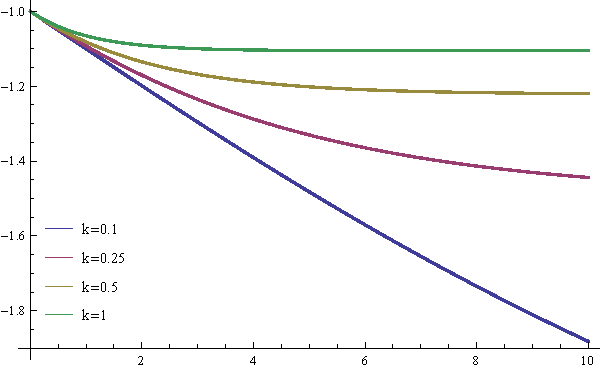
\includegraphics[width=8cm]{slike/gompertzova-rast}
      \end{center}
      \caption{Vzeli smo $h_0=-1$ in $a_0=0,1$ in variirali $k=0,1;0,25;0,5;1$.}
      \label{fig:gompertzova-rast}
    \end{figure}

Po začetni hitrejši rasti, se količina $h(t)$ postopoma ustali pri asimptotski vrednosti in nam torej da dinamiko, ki ustreza našim zahtevam za vrtače. Zmanjšujočo se hitrost rasti bi lahko pripisali bolj učinkovitemu odvajanju vode skozi apnenec, zaradi česar bi se čas ko je voda v stiku s kamnino in jo lahko raztaplja zmanjšal.
Gompertzov model se recimo uporablja za modeliranje rasti slabo prekrvavljenih tumorjev. \cite{wheldon1988mathematical}

\begin{comment} 
\subsection{Komentar}
[TODO]Opis razlik in podobnosti med temi modeli deterministične dinamike[TODO]
\end{comment}

    \section{Difuzijsko modeliranje dinamike vrtač}

V prejšnjem poglavju predlagane deterministične nastavke dinamike sedaj zaporedno vstavljamo v splošno reakcijsko-difuzijsko enačbo (\ref{dinamicna-splosna}) in jo numerično rešujemo pri robnih pogojih (\ref{rd-robni}). Omejimo se na eno dimenzijo, $x$, ki nam pove kje v prerezu vrtače se nahajamo, višino $h(t,x)$, ki nam pove višino površja v točki $x$ ob času $t$ in čas $t$. Rešitve prikažemo in komentiramo njeno časovno dinamiko. Izbrani robni pogoji

    \begin{equation}
      \begin{aligned}
        h(0,x) =  - e^{-x^2}, x \in D \\
        h(t,x) = 0, x \in \partial D \\
        \frac{\partial h(t,x)}{\partial n} = 0, x \in \partial D
      \end{aligned}
\label{rd-robni}
    \end{equation}
postavijo, da začnemo na ravni podlagi, z majhno udrtino Gaussove oblike. Vrednost $h(t,x)$ in njen prvi odvod po normali na robu območja postavimo na $0$.

Uporabljeni seti enačb in robnih pogojev so torej nelinearni in popolnoma deterministični, medtem ko smo pri Kardar-Parisi-Zhangovem modelu študirali stohastično a linearno rast.
    \subsection{Eksponentna rast}

Model eksponentne rasti z difuzijo postavi, da je rast linearno odvisna od stanja sistema in difuzije. Mehanizma, ki bi rast ustavljal ni.
    \begin{equation}
      \frac{ \partial h(t,x) }{ \partial t} = D \frac{\partial^2}{\partial x^2} h(t,x) + a \cdot h(t,x).
      \label{difuzija-eksponentna-rast}
    \end{equation}

Sistem nam da eksponentno rast, kot je prikazano na (Slika \ref{fig:difuzija-eksponentna-rast}).
Eksponenta rast z difuzijo je v določenem intervalu smiseln model za opis populacije virusov ali verižnih jedrskih reakcij. Za rast vrtač bi bila lahko primeren model le v kratkem obdobju v začetku nastajanja vrtače, kasneje pa nikakor ne saj zelo globokih vrtač v naravi ne opazimo.
    \begin{figure}[h!]
      \begin{center}
        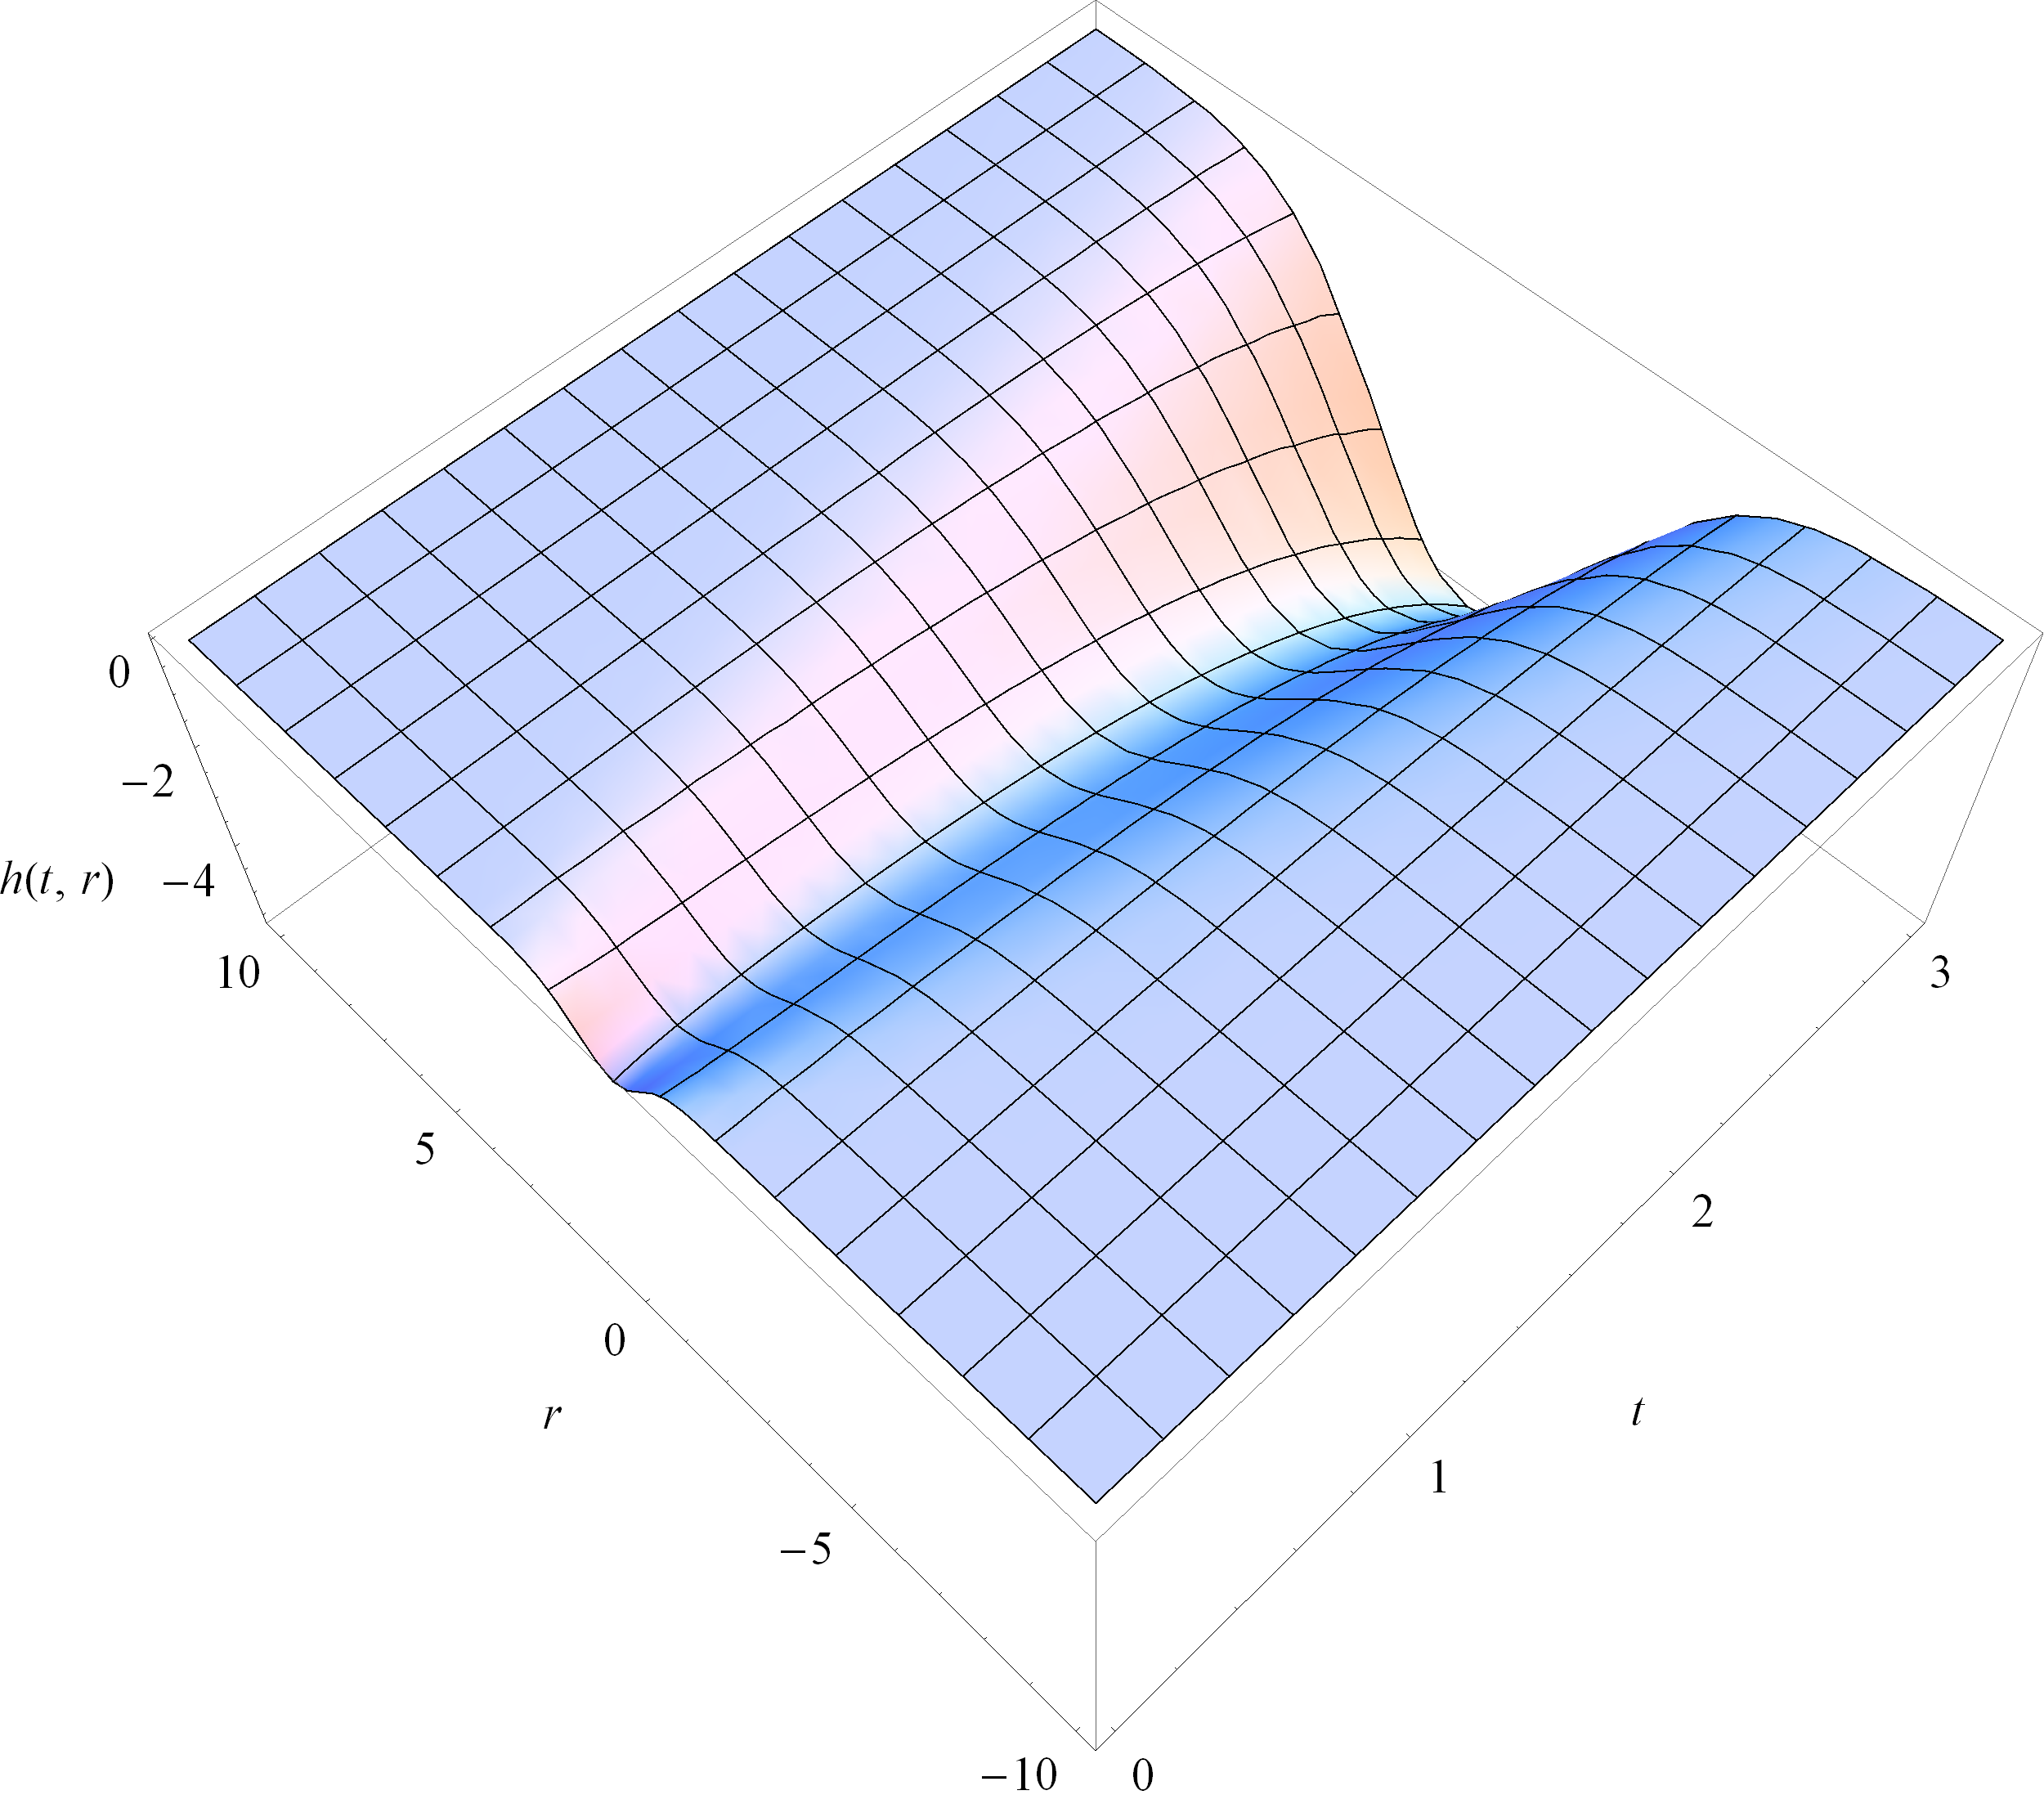
\includegraphics[width=7cm]{slike/difuzija-eksponentna-rast2}
      \end{center}
      \caption{Prikaz časovnega razvoja površja po modelu eksponentne rasti z difuzijskim členom, podanim z (\ref{difuzija-eksponentna-rast}). Vzeli smo $D=1$, $a=1$.}
      \label{fig:difuzija-eksponentna-rast}
    \end{figure}

\subsection{Omejena eksponentna rast}

    Omejena eksponentna rast z difuzijo upošteva nosilno kapaciteto sistema in se uporablja za opis modelov, kjer znotraj populacije ni interakcij. Na primer pri širjenju v družbi preko medijev, brez medosebnega prenosa.\\

    \begin{equation}
      \frac{ \partial h(t,x) }{ \partial t} = D \frac{\partial^2}{\partial x^2} h(t,x) + a \cdot (K - h(t,x)).
      \label{difuzija-omejena-eksponentna-rast}
    \end{equation}
    \begin{figure}[h]
      \begin{center}
        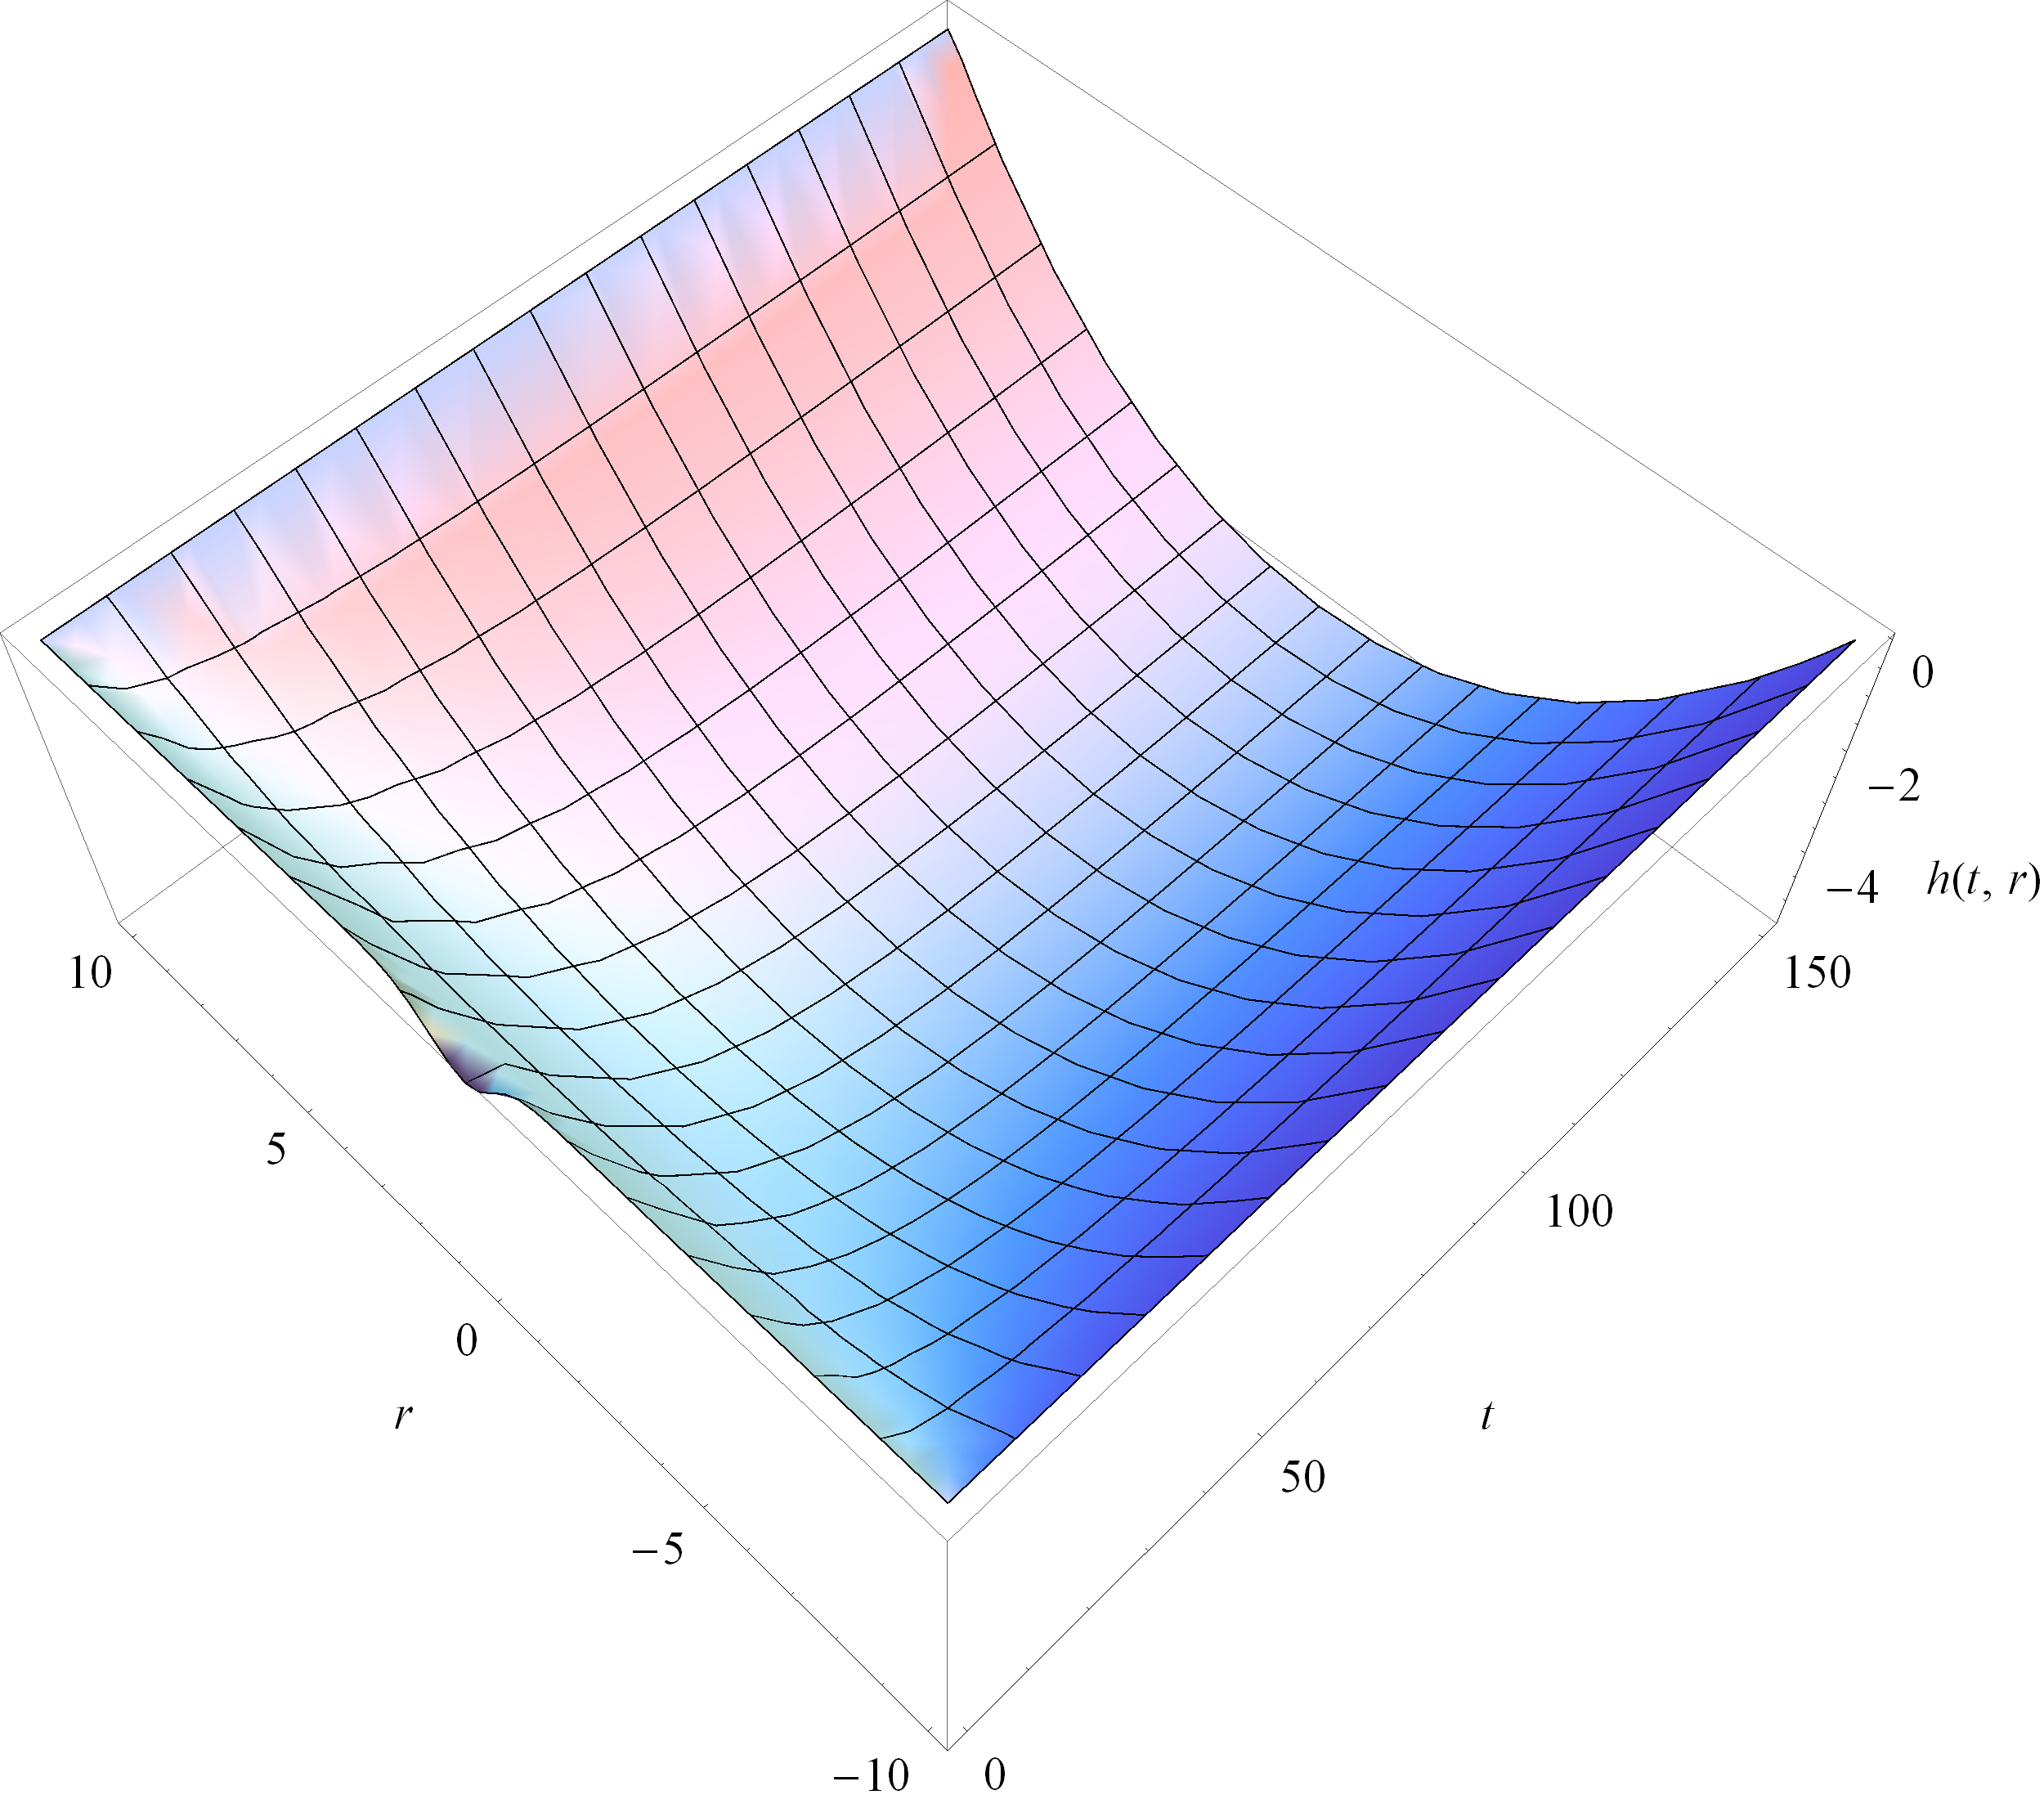
\includegraphics[width=7cm]{slike/difuzija-omejena-eksponentna-rast2}
      \end{center}
      \caption{Prikaz časovnega razvoja površja po modelu omejene eksponentne rasti z difuzijskim členom, podanim z (\ref{difuzija-omejena-eksponentna-rast}). Vzeli smo $D=1$, $a=\frac{1}{50}$, $K=-10$.}
      \label{fig:difuzija-omejena-eksponentna-rast}
    \end{figure}

    Dobljena rast (Slika \ref{fig:difuzija-omejena-eksponentna-rast}) eksponentno raste do praga K, kjer se zasiti. Rast v začetku je hitra. Pri vrtačah v začetku pričakujemo počasnejšo rast, saj se mora najprej vzpostaviti učinkovita mreža za odvajanje vode. Zaradi tega se model ne zdi najbolj verjeten kandidat za dinamiko vrtač.


    \subsection{Logistična rast}
Logistična rast z difuzijo nam da Fisher-Kolmogorovo enačbo, ki se uporablja v populacijski genetiki in predstvalja časovno-prostorsko rast populacije ob končnih prehrambenih kapacitetah okolja:

    \begin{equation}
      \frac{ \partial h(t,x) }{ \partial t} = D \frac{\partial^2}{\partial x^2} h(t,x) + a \cdot h(t,x) \cdot (1 - \frac{h(t,x)}{K}).
      \label{difuzija-logisticna-rast}
    \end{equation}
    \begin{figure}[h!]
      \begin{center}
        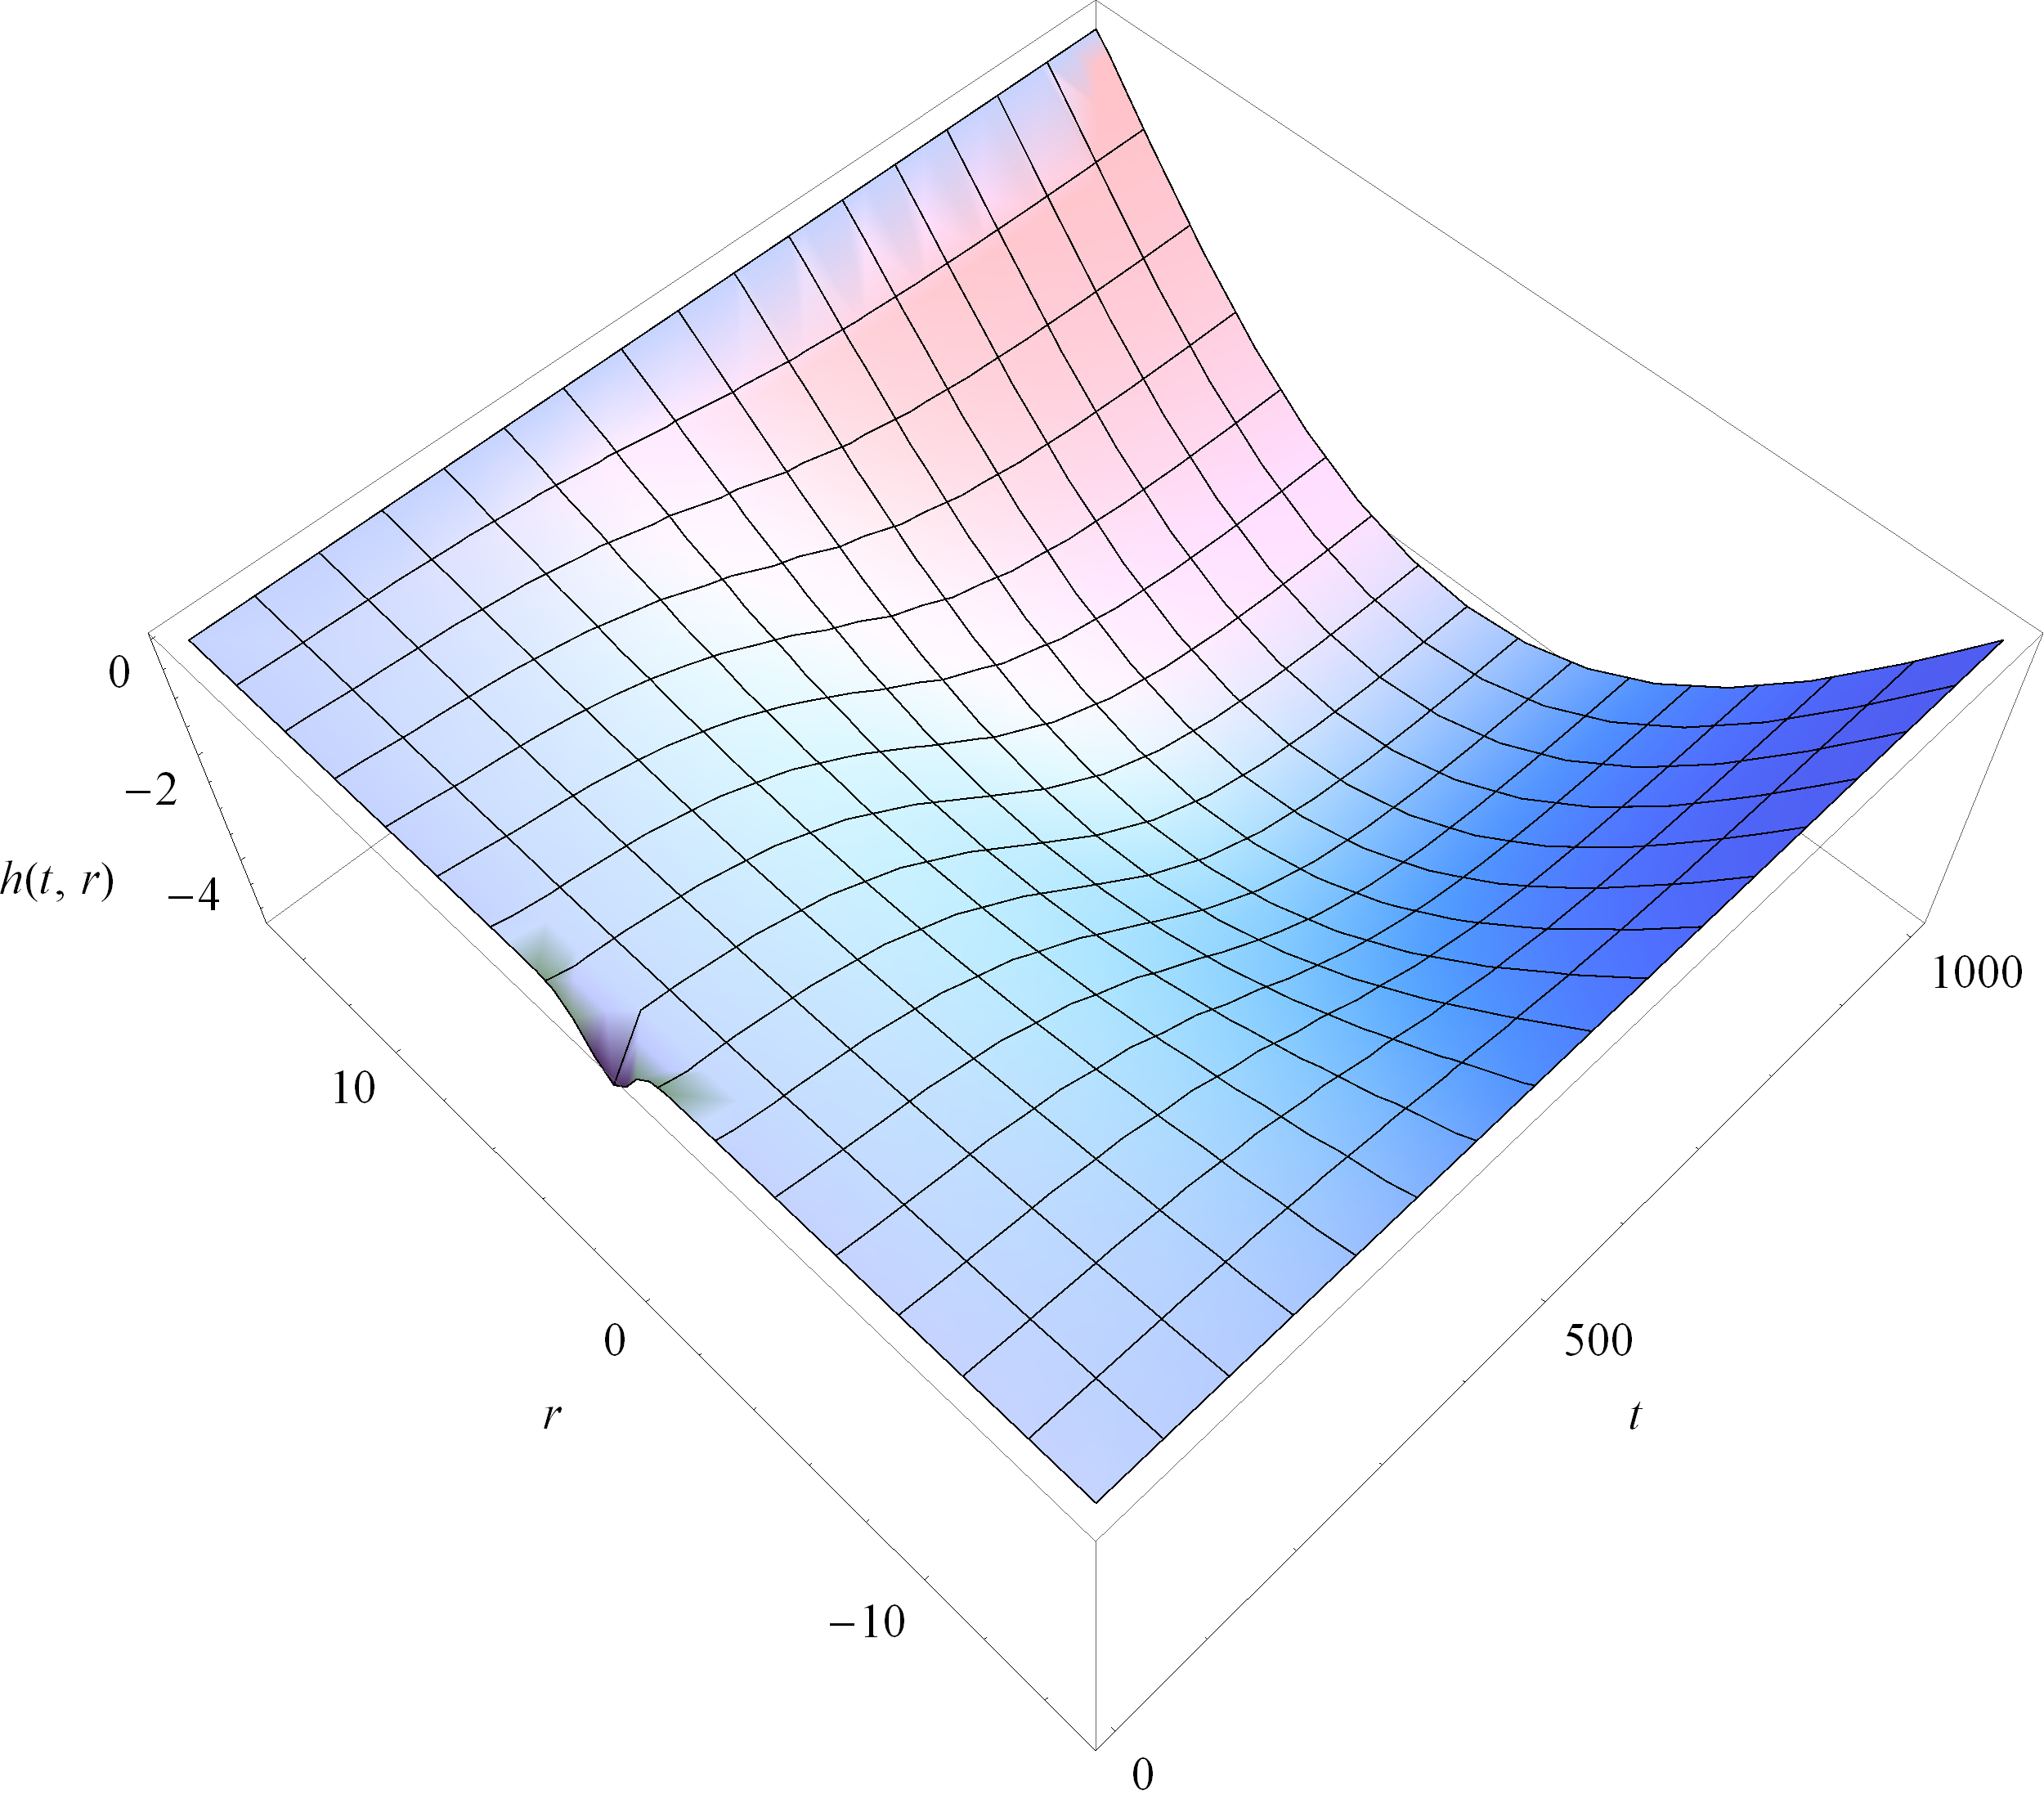
\includegraphics[width=9cm]{slike/difuzija-logisticna-rast2}
      \end{center}
      \caption{Prikaz časovnega razvoja površja po modelu logistične rasti z difuzijskim členom, podanim z (\ref{difuzija-logisticna-rast}).Vzeli smo $D=1$, $a=\frac{1}{50}$, $K=-10$.}
      \label{fig:difuzija-logisticna-rast}
    \end{figure}

Fisher je ta model originalno predlagal za opis širjenja ugodnih genov po populaciji \cite{broadbridge2002huxley}. Parameter $a$ je bil v tem kontekstu metrika za koristnost gena. Model se uporablja še za opis širjenja človeških populacij po originalno praznih območjih, npr. naselitev Severne Amerike.\\

Rešitve Fisher-Kolmorgorove enačbe (\ref{difuzija-logisticna-rast}) imajo pomembno lastnost, ki jo ostali hipotetični modeli rasti vrtač nimajo, in sicer vodijo do intrinzične velikosti končnega profila površine, ki ni odvisen od robnih pogojev, kot pri vseh ostalih modelih. Dejansko vodijo do nastanka dinamične fronte, ki se pomika kot val po sistemu. Ta lastnost enačbe Fisher-Kolmorgorova je dobro znana tudi v populacijski genetiki. Običajno nastanek takih stabilnih profilov v reakcijsko-difuzijskih sistemih imenujemo tudi samoorganizacija.

Ko se pobočje enkrat oblikuje, ne spreminja več oblike, ampak potuje kot valovna fronta navzven (Slika \ref{fig:difuzija-logisticna-rast}). Pokažemo lahko, da je dolžina vala odvisna od difuzijske konstante $D$ in faktorja rasti $a$, ter da velja: 
    \[ \lambda \sim \sqrt{D/a}. \]
Iz te zveze lahko pokažemo tudi, da je hitrost takega vala $v = 2 \sqrt{D a}$.

Logistična rast z difuzijo, ki omogoča samoorganizacijo profila vrtače, nam da dober model za dinamiko vrtač. Začetna rast je počasna, nato se pohitri in končno ustali, kar pričakujemo iz geomorfološke skice (Slika \ref{fig:vrtaca-ford-williams}) - v začetku homogena podlaga postopoma vedno bolje odvaja vodo in na koncu procesa z dobrim odvajanjem ter neprepustno prstjo stabilizira vrtačo v neki končni obliki.
Velikost pobočja je za razliko od ostalih reakcijsko-difuzijskih modelov intrinzična lastnost in ne določena z robnimi pogoji, kot pri ostalih modelih. To se zdi po opazovanju vrtač v naravi bolj smiselno.

    \subsection{Gompertzova rast}

    Deterministični model Gompertzove rasti z difuzijskim členom nam da:

    \begin{equation}
      \frac{ \partial h(t,x) }{ \partial t} = D \frac{\partial^2}{ \partial x^2} h(t,x) - h(t,x) \cdot e^{-a t}.
      \label{difuzija-gompertzova-rast}
    \end{equation}
    \begin{figure}[h]
      \begin{center}
        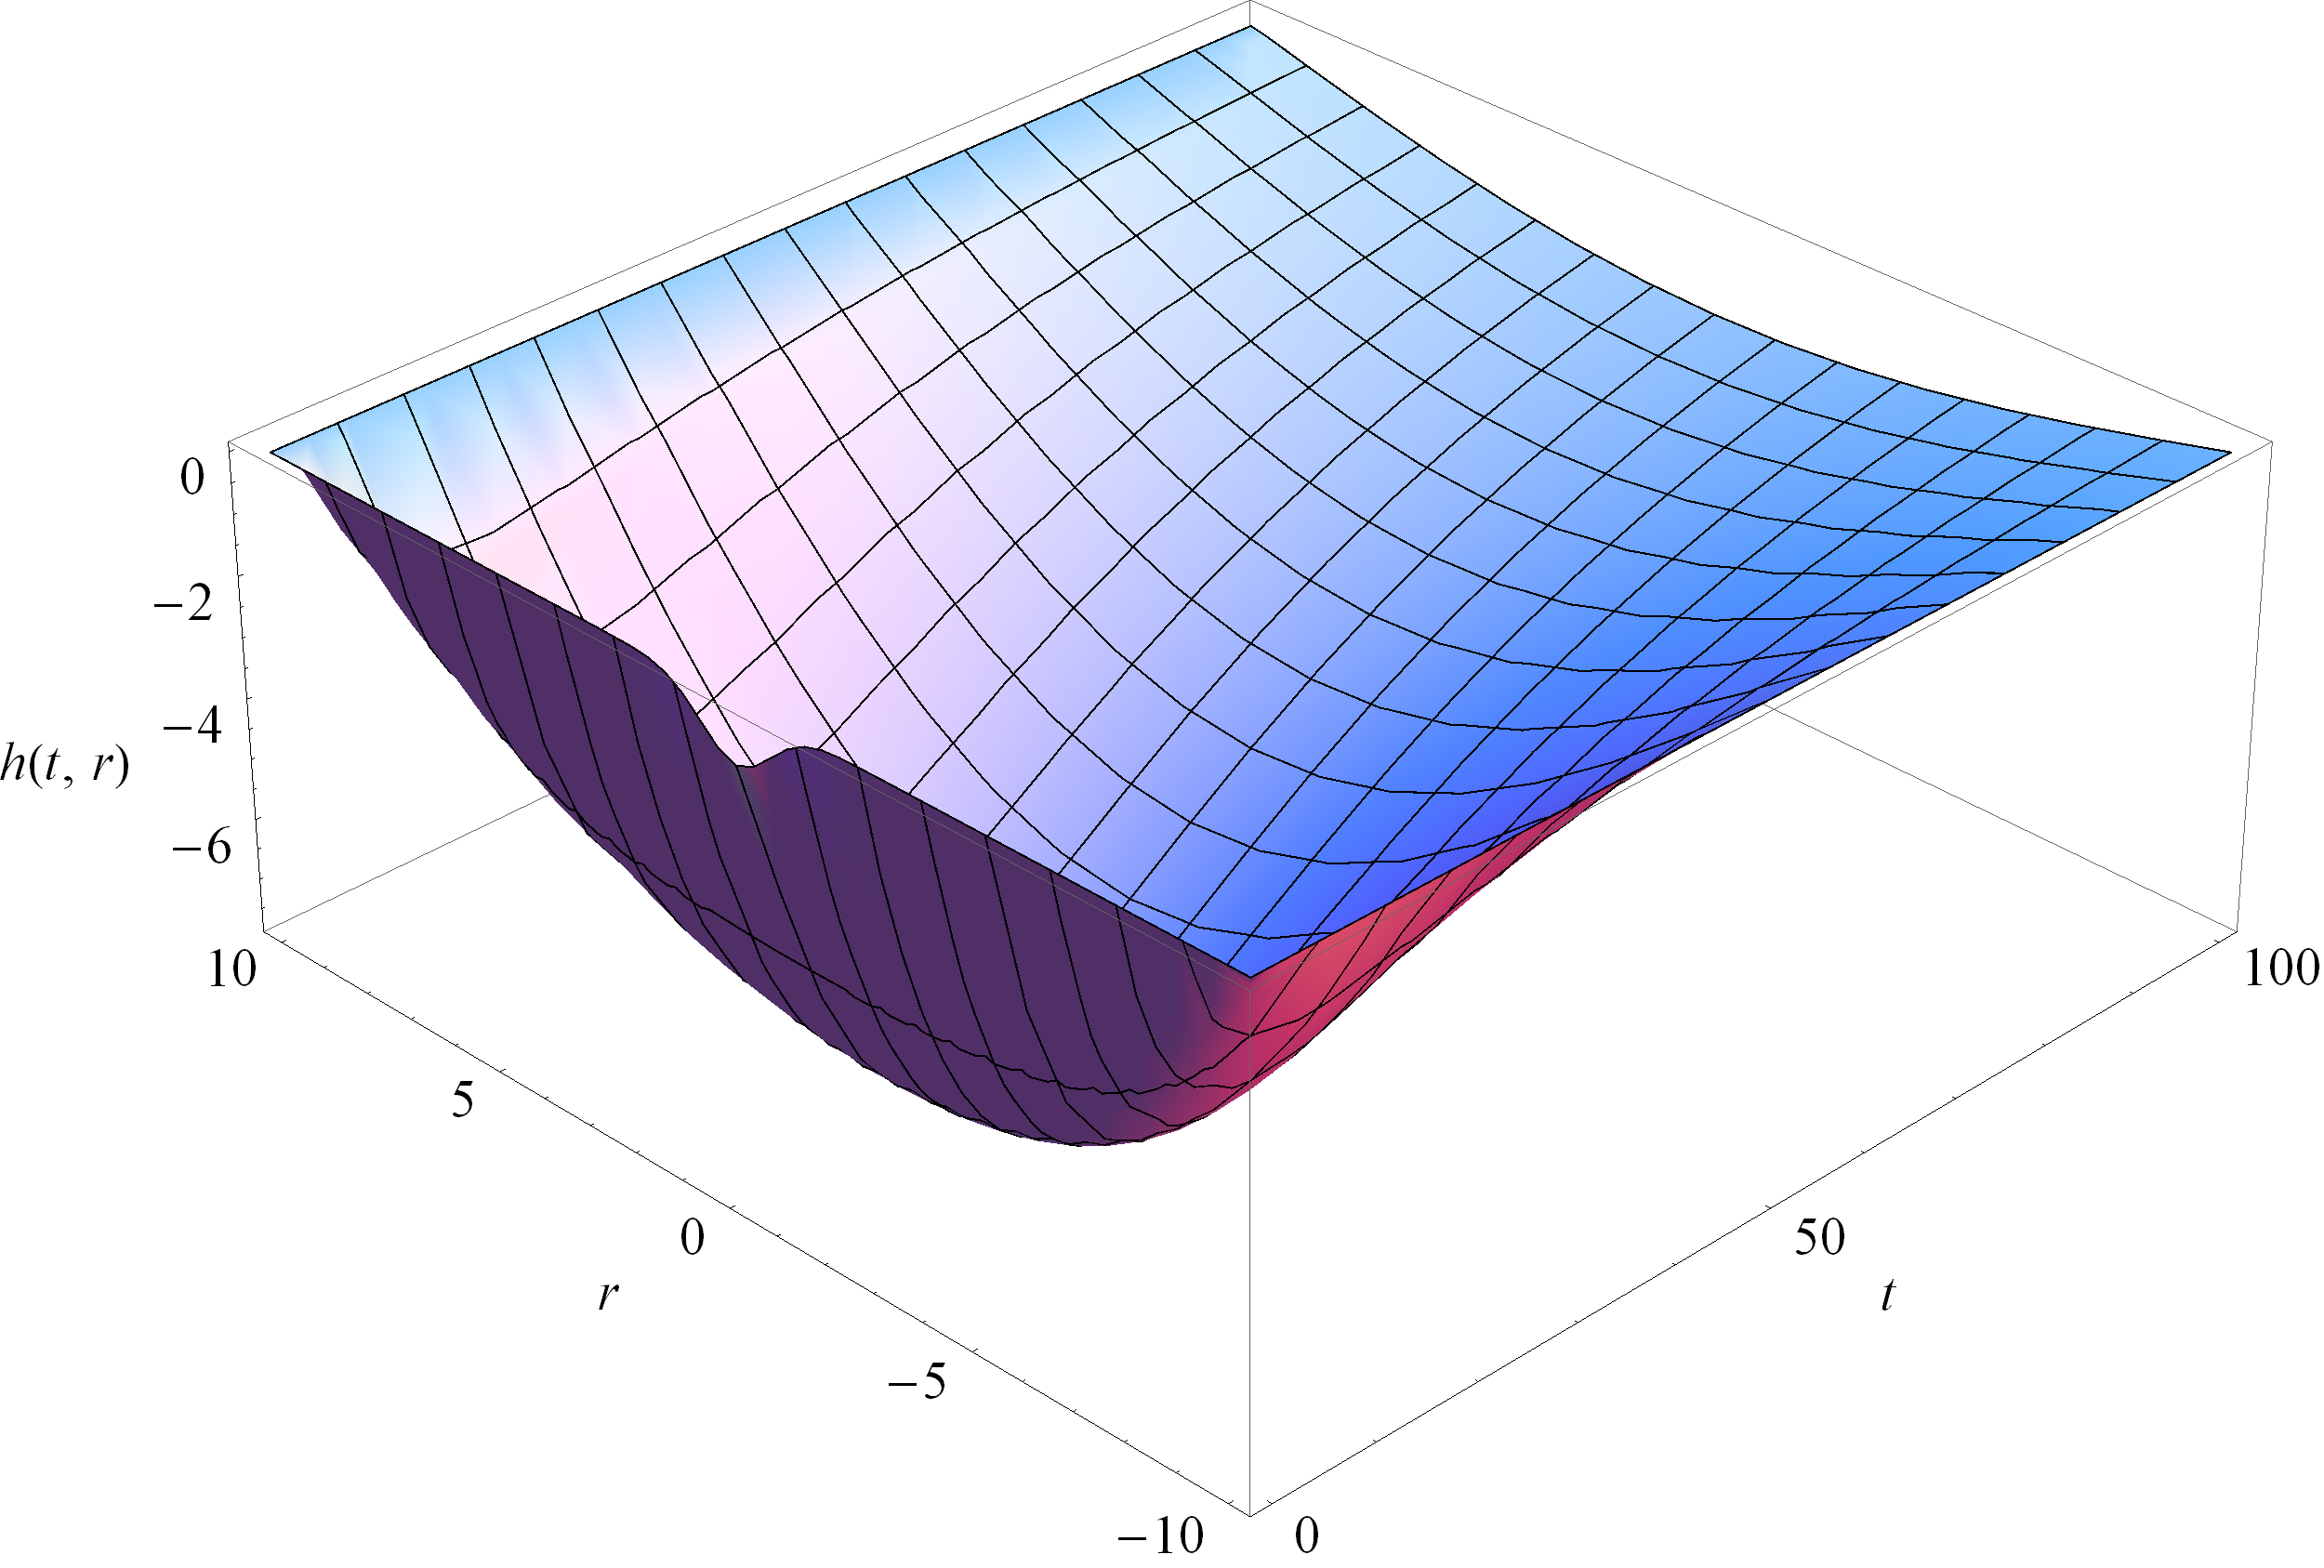
\includegraphics[width=9cm]{slike/difuzija-gompertzova-rast2}
      \end{center}
      \caption{Vzeli smo $D=1$, $a=\frac{1}{10}$.}
      \label{fig:difuzija-gompertzova-rast}
    \end{figure}

    Vidimo, da rast tokrat s časom upada (Slika \ref{fig:difuzija-gompertzova-rast}). Tako profil najprej zraste, nato pa se difuzijsko izravna, ko difuzija prevlada.
    Model bi lahko upravičevali z idejo, da se z rastjo učinkovitejših odvodnih kanalov voda manj zadržuje v vrtači in se rast posledično upočasni. Vendar nimamo dovolj podatkov, da bi to idejo resno komentirali. Poleg tega nam model ne da stabilne oblike vrtače in se zato zdi za modeliranje vrtač neprimeren.

\subsection{Primerjava reakcijsko-difuzijskih modelov}

Vse predlagane modele vrtač lahko podamo z variiranjem nastavka $F(h)$ v difuzijski enačbi:
\begin{equation}
  \frac{ \partial h(t,x) }{ \partial t} = D \nabla^2 h + F(h).
  \label{dinamicna-splosna3}
\end{equation}

Od fenomenoloških reakcijsko difuzijskih enačb, pridobljenih z determinističnim nastavkom $F(h)$, sta najbolj obetavna modela omejena eksponentna in logistična rast. Pri previdno izbranih robnih pogojih dajo intuitivno sprejemljive rezultate, pri čemer se logistična rast zdi bolj smiselna glede na geomorfološko literaturo. Zanimiva lastnost logistične difuzijske rasti je tudi oblika pobočja, ki je neodvisna od robnih pogojev.
Rezultata eksponentne in Gompertzove rasti po dolgem času nista skladna z opažanji v naravi.

Za deterministični model rasti vrtače torej na osnovi opisanih lastnosti različnih predstavljenih modelov predlagamo tistega, ki temelji na Fisher-Kolmogorovi reakcijsko-difuzijski enačbi:
\begin{equation}
  \frac{ \partial h}{ \partial t} = D \nabla^2 h + a \cdot h (1 - \frac{h}{K}).
  \label{dinamicna-splosna4}
\end{equation}

Determinističen reakcijsko-difuzijski model bi bil uporaben za modeliranje ene same vrtače, a ker nima nobene stohastične komponente z njim ne moremo pristopati k analizi populacije vrtač, ki sicer ustrezajo istemu modelu rasti, a s stohastično variacijo parametrov, ki v teh modelih nastopajo. Stohastično komponento modeliranja denudacije kraškega površja pač bolje izrazi Kardar-Parisi-Zhang model, ki temelji na linearni rasti z velikostjo, ki jo podaja Gaussov šum. S primerjavo izmerjene in po modelu pričakovane hrapavosti površja, smo pokazali da je Kardar-Parisi-Zhangov model morda primeren za opis dinamike vrtač. Morda bi bil najustreznejši model za opis vrtač Fisher-Kolmogorova enačba, a s stohastično velikostjo dinamike:
\begin{equation}
  \frac{ \partial h}{ \partial t} = D \nabla^2 h + \eta(\mathbf{x},t) \cdot h(1 - \frac{h}{K}),
  \label{dinamicna-splosna5}
\end{equation}
ki pa zahteva poglobljeno analizo v okviru teorije stohastičnih procesov in je v tem delu ne bomo nadaljevali.

    \chapter{Zaključek}

    Izkaže se, da je zaznava in segmentacija vrtač na digitalnem modelu reliefa relativno enostavna naloga, izvedljiva na osebnem računalniku. Kodo, ki sem jo za ta postopek spisal, sem dokumentirano objavil na spletu in bo morda služila za obsežnejšo katalogizacijo vrtač.
    Za nekoliko težjo nalogo se izkaže določanje idealne oblike vrtače, saj le-ta v naravi ne obstaja. Pravo vprašanje bi se moralo glasiti, kakšna je idealna oblika vrtače na izotropni podlagi po dolgem času. Vseeno sem se odločil, da za idealno vrtačo vzamem povprečje velike količine vrtač.

    Precej zahtevnejša naloga je izbira fizikalnega modela in dinamičnega opisa vrtače zaradi omejene količine podatkov o časovni dinamiki (domnevali smo, da so vse vrtače že v ravnovesnem stanju) in nepoznavanja dejanskega procesa, ki znižuje površje.

    Pri modeliranju smo vedno predpostavili difuzijo in različne vplive, ki bi jih prisotnost vrtače na kraškem površju lahko imela na raztapljanje površja. Poleg determinističnih modelov rasti, smo predlagali tudi stohastičnega.

    Stohastičnen model Kardar-Parisi-Zhangove rasti površin nam da rezultat podoben kraškemu površju z vrtačami. Simulirano površje pa je kvalitativno podobno realnim površjem z vrtačami. Teoretično napovedan eksponent hrapavosti se relativno dobro ujema z izmerjenim na področju Menišije. Tega rezultata ne moremo obravnavati kot dokaz, morda le spodbudo za nadaljnji študij. Zanimiv nadaljnji korak bi bil študij statistike dimenzij konkavnih objektov na simuliranem površju.

    Kot determinističen model dinamike rasti posamezne vrtače se posebno odlikuje model logistične rasti z difuzijo (\ref{fig:difuzija-logisticna-rast}), ki da časovno najbolj smiseln potek rasti vrtače. Intrinzična lastnost modela je tudi oblika pobočij vrtač, kar od dobrega modela vrtače vsekakor pričakujemo. Odprto ostaja vprašanje robnih pogojev - če ta model velja, kaj omejuje velikost vrtač?

    Za popolnejši študij in dober model vrtač bi verjetno potrebovali bolj poglobljene informacije o prsti, geoloških in bioloških dejavnikih, ki lahko vplivajo na časovno dinamiko terena.

Zanimiva ideja bi bila z geološkim študijem najti in datirati vrtače v različnih stopnjah razvoja ter s pomočjo te informacije oblikovati dinamičen nastavek, na podlagi katerega bi potem morda bolj osvetlili dinamično enačbo.

Dobro razumevanje nastanka in dinamike vrtač bi nam lahko omogočilo preprosto geološko datacijo različnih kraških površij, na podlagi gostote vrtač, ali pa porazdelitvi njihovih globini oziroma površin. Na podoben način astronomi datirajo površja na planetih. Privzamejo stalen pritok meteoritov z nekakšno stalno porazdelitvijo velikosti in iz gostote kraterjev datirajo starost izbranega površja. \cite{trey2011size}

    \newpage \thispagestyle{empty}


    \nocite{*}
    \newpage
    \bibliography{bibliography}{}
    \addcontentsline{toc}{chapter}{Literatura}
    \bibliographystyle{alpha}

    \newpage \thispagestyle{empty}



    \vspace*{1cm}
    \begin{center} {\Large \textbf{\sc Izjava o avtorstvu in objavi elektronske oblike zaključnega dela: }} \end{center}

      \vspace{1cm} \noindent Podpisani Rok Mihevc izjavljam:
      \noindent 

      \begin{itemize}
        \item 
          da sem diplomsko delo z naslovom \emph{Kraške vrtače Dinarskega krasa} izdelal samostojno pod mentorstvom prof.\ dr.\ \mbox{Rudolfa} \mbox{Podgornika} in
        \item
          da Fakulteti za matematiko in fiziko Univerze v Ljubljani dovoljujem objavo elektronske 
          oblike svojega dela na spletnih straneh.
      \end{itemize}

      \vspace{1cm} \noindent Ljubljana, 18. april 2014 \hfill Podpis avtorja:


      \end{document}

